\documentclass[tocnosub,noragright,centerchapter,12pt]{uiucecethesis09}
% Use draftthesis for notes and date markings on every page.  Useful when you
%   have multiple copies floating around.
% Use offcenter for the extra .5 inch on the left side. Needed with fullpage and fancy.
% Use mixcasechap for compatibility with hyperref package, which does NOT like all caps default
% Use edeposit for the adviser/committee on the title page.
% Use tocnosub to suppress subsection and lower entries in the TOC.
% PhD candidates use "proquest" for the proquest abstract.

\makeatletter

\usepackage{setspace}
%\usepackage{epsfig}  % for figures
\usepackage{graphicx}  % another package that works for figures
\usepackage{multirow}
\usepackage{placeins}
\usepackage{caption}  % allows center figures caption
\usepackage{booktabs} % nice rules (thick lines) for tables
\usepackage{array}
\usepackage{tabularx}
\graphicspath{{figures/}}
%\usepackage{subfigure}  % for subfigures
\usepackage{amsmath}  % for math spacing
%\usepackage{amssymb}  % for math spacing
%\usepackage{url}  % Hyphenation of URLs.
\usepackage{lscape}  % Useful for wide tables or figures.
\usepackage[justification=raggedright]{caption}	% makes captions ragged right - thanks to Bryce Lobdell
\usepackage[acronym,toc]{glossaries}  % acronyms inclusion
\usepackage{color,soul}
\makeglossary

% Uncomment the appropriate one of the following four lines:
\msthesis
%\phdthesis
%\otherdoctorate[abbrev]{Title of Degree}
%\othermasters[abbrev]{Title of Degree}

\title{Advanced online fuel reprocessing simulation for thorium-fueled Molten Salt Breeder Reactor}
\author{Andrei Rykhlevskii}
\department{the Department of Nuclear, Plasma, and Radiological Engineering}
\degreeyear{2018}

% Advisor name is required for
% - doctoral students for the ProQuest abstract
% - master's students who do not have a master's committee
%\advisor{Professor Kathryn D. Huff}

% Uncomment the \committee command for
% - all doctoral students
% - master's students who have a master's committee
\committee{Assistant Professor Kathryn Huff, Chair\\
           Associate Professor Tomasz Kozlowski} % etc.

\begin{document}
%\newacronym{<++>}{<++>}{<++>}
\newacronym[longplural={metric tons of heavy metal}]{MTHM}{MTHM}{metric ton of heavy metal}
\newacronym{ABM}{ABM}{agent-based modeling}
\newacronym{ACDIS}{ACDIS}{Program in Arms Control \& Domestic and International Security}
\newacronym{AHTR}{AHTR}{Advanced High Temperature Reactor}
\newacronym{ANDRA}{ANDRA}{Agence Nationale pour la gestion des D\'echets RAdioactifs, the French National Agency for Radioactive Waste Management}
\newacronym{ANL}{ANL}{Argonne National Laboratory}
\newacronym{ANS}{ANS}{American Nuclear Society}
\newacronym{API}{API}{application programming interface}
\newacronym{ARE}{ARE}{Aircraft Reactor Experiment}
\newacronym{ARFC}{ARFC}{Advanced Reactors and Fuel Cycles}
\newacronym{ASME}{ASME}{American Society of Mechanical Engineers}
\newacronym{ATWS}{ATWS}{Anticipated Transient Without Scram}
\newacronym{BDBE}{BDBE}{Beyond Design Basis Event}
\newacronym{BIDS}{BIDS}{Berkeley Institute for Data Science}
\newacronym{CAFCA}{CAFCA}{ Code for Advanced Fuel Cycles Assessment }
\newacronym{CDTN}{CDTN}{Centro de Desenvolvimento da Tecnologia Nuclear}
\newacronym{CEA}{CEA}{Commissariat \`a l'\'Energie Atomique et aux \'Energies Alternatives}
\newacronym{CI}{CI}{continuous integration}
\newacronym{CNEN}{CNEN}{Comiss\~{a}o Nacional de Energia Nuclear}
\newacronym{CNERG}{CNERG}{Computational Nuclear Engineering Research Group}
\newacronym{COSI}{COSI}{Commelini-Sicard}
\newacronym{COTS}{COTS}{commercial, off-the-shelf}
\newacronym{CSNF}{CSNF}{commercial spent nuclear fuel}
\newacronym{CTAH}{CTAHs}{Coiled Tube Air Heaters}
\newacronym{CUBIT}{CUBIT}{CUBIT Geometry and Mesh Generation Toolkit}
\newacronym{CURIE}{CURIE}{Centralized Used Fuel Resource for Information Exchange}
\newacronym{DAG}{DAG}{directed acyclic graph}
\newacronym{DANESS}{DANESS}{Dynamic Analysis of Nuclear Energy System Strategies}
\newacronym{DBE}{DBE}{Design Basis Event}
\newacronym{DESAE}{DESAE}{Dynamic Analysis of Nuclear Energy Systems Strategies}
\newacronym{DHS}{DHS}{Department of Homeland Security}
\newacronym{DOE}{DOE}{Department of Energy}
\newacronym{DRACS}{DRACS}{Direct Reactor Auxiliary Cooling System}
\newacronym{DRE}{DRE}{dynamic resource exchange}
\newacronym{DSNF}{DSNF}{DOE spent nuclear fuel}
\newacronym{DYMOND}{DYMOND}{Dynamic Model of Nuclear Development }
\newacronym{EBS}{EBS}{Engineered Barrier System}
\newacronym{EDF}{EDF}{Électricité de France}
\newacronym{EDZ}{EDZ}{Excavation Disturbed Zone}
\newacronym{EIA}{EIA}{U.S. Energy Information Administration}
\newacronym{EPA}{EPA}{Environmental Protection Agency}
\newacronym{EPR}{EPR}{European Pressurized Reactors}
\newacronym{EP}{EP}{Engineering Physics}
\newacronym{EU}{EU}{European Union}
\newacronym{FCO}{FCO}{Fuel Cycle Options}
\newacronym{FCT}{FCT}{Fuel Cycle Technology}
\newacronym{FEHM}{FEHM}{Finite Element Heat and Mass Transfer}
\newacronym{FEPs}{FEPs}{Features, Events, and Processes}
\newacronym{FHR}{FHR}{Fluoride-Salt-Cooled High-Temperature Reactor}
\newacronym{FLiBe}{FLiBe}{Fluoride-Lithium-Beryllium}
\newacronym{FP}{FP}{Fission Products}
\newacronym{GDSE}{GDSE}{Generic Disposal System Environment}
\newacronym{GDSM}{GDSM}{Generic Disposal System Model}
\newacronym{GENIUSv1}{GENIUSv1}{Global Evaluation of Nuclear Infrastructure Utilization Scenarios, Version 1}
\newacronym{GENIUSv2}{GENIUSv2}{Global Evaluation of Nuclear Infrastructure Utilization Scenarios, Version 2}
\newacronym{GENIUS}{GENIUS}{Global Evaluation of Nuclear Infrastructure Utilization Scenarios}
\newacronym{GPAM}{GPAM}{Generic Performance Assessment Model}
\newacronym{GRSAC}{GRSAC}{Graphite Reactor Severe Accident Code}
\newacronym{GUI}{GUI}{graphical user interface}
\newacronym{HLW}{HLW}{high level waste}
\newacronym{HPC}{HPC}{high-performance computing}
\newacronym{HTC}{HTC}{high-throughput computing}
\newacronym{HTGR}{HTGR}{High Temperature Gas-Cooled Reactor}
\newacronym{IAEA}{IAEA}{International Atomic Energy Agency}
\newacronym{IEMA}{IEMA}{Illinois Emergency Mangament Agency}
\newacronym{IHLRWM}{IHLRWM}{International High Level Radioactive Waste Management}
\newacronym{INL}{INL}{Idaho National Laboratory}
\newacronym{IPRR1}{IRP-R1}{Instituto de Pesquisas Radioativas Reator 1}
\newacronym{IRP}{IRP}{Integrated Research Project}
\newacronym{ISFSI}{ISFSI}{Independent Spent Fuel Storage Installation}
\newacronym{ISRG}{ISRG}{Independent Student Research Group}
\newacronym{JFNK}{JFNK}{Jacobian-Free Newton Krylov}
\newacronym{LANL}{LANL}{Los Alamos National Laboratory}
\newacronym{LBNL}{LBNL}{Lawrence Berkeley National Laboratory}
\newacronym{LCOE}{LCOE}{levelized cost of electricity}
\newacronym{LDRD}{LDRD}{laboratory directed research and development}
\newacronym{LFR}{LFR}{Lead-Cooled Fast Reactor}
\newacronym{LLNL}{LLNL}{Lawrence Livermore National Laboratory}
\newacronym{LMFBR}{LMFBR}{Liquid Metal Fast Breeder Reactor}
\newacronym{LOFC}{LOFC}{Loss of Forced Cooling}
\newacronym{LOHS}{LOHS}{Loss of Heat Sink}
\newacronym{LOLA}{LOLA}{Loss of Large Area}
\newacronym{LP}{LP}{linear program}
\newacronym{LWR}{LWR}{Light Water Reactor}
\newacronym{MAGNOX}{MAGNOX}{Magnesium Alloy Graphie Moderated Gas Cooled Uranium Oxide Reactor}
\newacronym{MA}{MA}{minor actinide}
\newacronym{MCNP}{MCNP}{Monte Carlo N-Particle code}
\newacronym{MILP}{MILP}{mixed-integer linear program}
\newacronym{MIT}{MIT}{the Massachusetts Institute of Technology}
\newacronym{MOAB}{MOAB}{Mesh-Oriented datABase}
\newacronym{MOOSE}{MOOSE}{Multiphysics Object-Oriented Simulation Environment}
\newacronym{MOX}{MOX}{mixed oxide}
\newacronym{MSBR}{MSBR}{Molten Salt Breeder Reactor}
\newacronym{MSRE}{MSRE}{Molten Salt Reactor Experiment}
\newacronym{MSR}{MSR}{Molten Salt Reactor}
\newacronym{NAGRA}{NAGRA}{National Cooperative for the Disposal of Radioactive Waste}
\newacronym{NEAMS}{NEAMS}{Nuclear Engineering Advanced Modeling and Simulation}
\newacronym{NEUP}{NEUP}{Nuclear Energy University Programs}
\newacronym{NFCSim}{NFCSim}{Nuclear Fuel Cycle Simulator}
\newacronym{NGNP}{NGNP}{Next Generation Nuclear Plant}
\newacronym{NMWPC}{NMWPC}{Nuclear MW Per Capita}
\newacronym{NNSA}{NNSA}{National Nuclear Security Administration}
\newacronym{NPP}{NPP}{Nuclear Power Plant}
\newacronym{NPRE}{NPRE}{Department of Nuclear, Plasma, and Radiological Engineering}
\newacronym{NQA1}{NQA-1}{Nuclear Quality Assurance - 1}
\newacronym{NRC}{NRC}{Nuclear Regulatory Commission}
\newacronym{NSF}{NSF}{National Science Foundation}
\newacronym{NSSC}{NSSC}{Nuclear Science and Security Consortium}
\newacronym{NUWASTE}{NUWASTE}{Nuclear Waste Assessment System for Technical Evaluation}
\newacronym{NWF}{NWF}{Nuclear Waste Fund}
\newacronym{NWTRB}{NWTRB}{Nuclear Waste Technical Review Board}
\newacronym{OCRWM}{OCRWM}{Office of Civilian Radioactive Waste Management}
\newacronym{ORION}{ORION}{ORION}
\newacronym{ORNL}{ORNL}{Oak Ridge National Laboratory}
\newacronym{PARCS}{PARCS}{Purdue Advanced Reactor Core Simulator}
\newacronym{PBAHTR}{PB-AHTR}{Pebble Bed Advanced High Temperature Reactor}
\newacronym{PBFHR}{PB-FHR}{Pebble-Bed Fluoride-Salt-Cooled High-Temperature Reactor}
\newacronym{PEI}{PEI}{Peak Environmental Impact}
\newacronym{PH}{PRONGHORN}{PRONGHORN}
\newacronym{PRIS}{PRIS}{Power Reactor Information System}
\newacronym{PRKE}{PRKE}{Point Reactor Kinetics Equations}
\newacronym{PSPG}{PSPG}{Pressure-Stabilizing/Petrov-Galerkin}
\newacronym{PWAR}{PWAR}{Pratt and Whitney Aircraft Reactor}
\newacronym{PWR}{PWR}{Pressurized Water Reactor}
\newacronym{PyNE}{PyNE}{Python toolkit for Nuclear Engineering}
\newacronym{PyRK}{PyRK}{Python for Reactor Kinetics}
\newacronym{QA}{QA}{quality assurance}
\newacronym{RDD}{RD\&D}{Research Development and Demonstration}
\newacronym{RD}{R\&D}{Research and Development}
\newacronym{RELAP}{RELAP}{Reactor Excursion and Leak Analysis Program}
\newacronym{RIA}{RIA}{Reactivity Insertion Accident}
\newacronym{RIF}{RIF}{Region-Institution-Facility}
\newacronym{SFR}{SFR}{Sodium-Cooled Fast Reactor}
\newacronym{SINDAG}{SINDA{\textbackslash}G}{Systems Improved Numerical Differencing Analyzer $\backslash$ Gaski}
\newacronym{SKB}{SKB}{Svensk K\"{a}rnbr\"{a}nslehantering AB}
\newacronym{SNF}{SNF}{spent nuclear fuel}
\newacronym{SNL}{SNL}{Sandia National Laboratory}
\newacronym{STC}{STC}{specific temperature change}
\newacronym{SUPG}{SUPG}{Streamline-Upwind/Petrov-Galerkin}
\newacronym{SWF}{SWF}{Separations and Waste Forms}
\newacronym{SWU}{SWU}{Separative Work Unit}
\newacronym{TRIGA}{TRIGA}{Training Research Isotope General Atomic}
\newacronym{TRISO}{TRISO}{Tristructural Isotropic}
\newacronym{TSM}{TSM}{Total System Model}
\newacronym{TSPA}{TSPA}{Total System Performance Assessment for the Yucca Mountain License Application}
\newacronym{ThOX}{ThOX}{thorium oxide}
\newacronym{UFD}{UFD}{Used Fuel Disposition}
\newacronym{UML}{UML}{Unified Modeling Language}
\newacronym{UOX}{UOX}{uranium oxide}
\newacronym{UQ}{UQ}{uncertainty quantification}
\newacronym{US}{US}{United States}
\newacronym{UW}{UW}{University of Wisconsin}
\newacronym{VISION}{VISION}{the Verifiable Fuel Cycle Simulation Model}
\newacronym{VVER}{VVER}{Voda-Vodyanoi Energetichesky Reaktor (Russian Pressurized Water Reactor)}
\newacronym{VV}{V\&V}{verification and validation}
\newacronym{WIPP}{WIPP}{Waste Isolation Pilot Plant}
\newacronym{YMR}{YMR}{Yucca Mountain Repository Site}

%%%%%%%%%%%%%%%%%%%%%%%%%%%%%%%%%%%%%%%%%%%%%%%%%%%%%%%%%%%%%%%%%%%%%%%%%%%%%%%
% TITLE
%
\maketitle

%\raggedright
\parindent 1em%

\frontmatter

%%%%%%%%%%%%%%%%%%%%%%%%%%%%%%%%%%%%%%%%%%%%%%%%%%%%%%%%%%%%%%%%%%%%%%%%%%%%%%%
% ABSTRACT
%
\begin{abstract}
% Put the abstract in a file called "abs.tex" and it'll be inputted here.
\vspace{-0.2in}
Current interest in advanced nuclear energy and \gls{MSR} concepts has enhanced demand in building the tools to analyze these systems. This thesis introduces a Python script, SaltProc, which simulates \gls{MSR} online reprocessing by modeling the changing isotopic composition of an irradiated fuel salt. SaltProc couples with the Monte Carlo code, SERPENT 2, for neutron transport and depletion calculations. SaltProc capabilities include a generic geometry capable of modeling multi-region and multi-flow systems, time-dependent feeds and removals, and specific separation efficiency for each element or isotope removal flow. Generally applicable  capabilities are illuminated in this thesis in three applied problems: (1) simulating the startup of a thorium-fueled \gls{MSBR} fuel cycle to find equilibrium fuel composition (when multiplication factor of the full-core model and the $^{233}$U concentration in the fuel salt are invariant in time); (2) determining the effect of the fuel salt irradiation with online reprocessing on \gls{MSBR} operations; and (3) estimating \gls{MSBR} fuel cycle performance by computing the $^{232}$Th feed rate over 20 years of operation and comparing with available data.

In the first application, full-core depletion in the \gls{MSBR} demonstrated that (1) equilibrium fuel composition could be achieved after 16 years and (2) the multiplication factor stabilizes after 6 years of operation. In the second application, fuel salt irradiation with simulated fission product removal and fissile/fertile feed causes considerable neutron energy spectrum hardening; this spectral shift has a problematic impact on safety parameters (e.g., temperature reactivity feedback, reactivity control system worth). In the third application, the average $^{232}$Th feed rate throughout 20 years of operation is 2.39 kg/day or 100 g/GWh$_e$ which is a good agreement with other recent research. Problematic effects of neutron energy spectrum hardening during \gls{MSBR} operation should be taken into account for neutronics, multi-physics, and fuel cycle performance analysis.
\end{abstract}

%%%%%%%%%%%%%%%%%%%%%%%%%%%%%%%%%%%%%%%%%%%%%%%%%%%%%%%%%%%%%%%%%%%%%%%%%%%%%%%
% DEDICATION
%
%\begin{dedication}
%Dedicated to the memory of my father, Igor Rykhlevskii, who always believed in %my ability to succeed in the academic arena.
%\end{dedication}

%%%%%%%%%%%%%%%%%%%%%%%%%%%%%%%%%%%%%%%%%%%%%%%%%%%%%%%%%%%%%%%%%%%%%%%%%%%%%%%
% ACKNOWLEDGMENTS
%
% Put acknowledgments in a file called "ack.tex" and it'll be inputted here.
%\begin{acknowledgments}
%I would like to express to my sincere gratitude towards my advisor Professor Kathryn Huff
for her valuable support throughout this project. She offered perpetual encouragement, patience and guidance
without which I would not have been able to complete this thesis. I would also like to thank Professor Tomasz Kozlowski and Professor Rizwan Uddin for their assessment and regarded perspectives in the review of this work. This work is also part of the "Advanced Reactors and Fuel Cycles" Petascale Computational Resource allocation support by the National Science Foundation.

I would also like to thank my colleagues Jin Whan Bae, Alex Lindsay, Gavin Ridley, Gyu Tae Park, Sun Myung Park, and Anshuman Chaube for their thoughts, discussion and help during research and writing of this work. I would like to recognize all the faculty and staff of the Nuclear, Plasma, and Radiological Engineering department who have continuously aided and guided me since my very first day in Champaign. 

Finally, I thank my wife Nelli Alivoryan and my daughters Sofiya and Zoe Annabelle for their limitless love and support. I have wholehearted thankfulness for my mother and my sisters who have always encouraged me in all my beginnings and without whom this work would not have been possible. 


%\end{acknowledgments}																																				
%%%%%%%%%%%%%%%%%%%%%%%%%%%%%%%%%%%%%%%%%%%%%%%%%%%%%%%%%%%%%%%%%%%%%%%%%%%%%%%
% TABLE OF CONTENTS
%
\tableofcontents

%%%%%%%%%%%%%%%%%%%%%%%%%%%%%%%%%%%%%%%%%%%%%%%%%%%%%%%%%%%%%%%%%%%%%%%%%%%%%%%
% LIST OF TABLES
%
% The List of Tables is not strictly necessary. Omitting the List of Tables will
% simplify the thesis check and reduce the number of corrections.
%\listoftables

%%%%%%%%%%%%%%%%%%%%%%%%%%%%%%%%%%%%%%%%%%%%%%%%%%%%%%%%%%%%%%%%%%%%%%%%%%%%%%%
% LIST OF FIGURES
%
% The List of Figures is not strictly necessary. Omitting the List of Figures will
% simplify the thesis check and reduce the number of corrections.
%\listoffigures

%%%%%%%%%%%%%%%%%%%%%%%%%%%%%%%%%%%%%%%%%%%%%%%%%%%%%%%%%%%%%%%%%%%%%%%%%%%%%%%
% LIST OF ABBREVIATIONS
%
% The List of Abbreviations is not strictly necessary.
%\chapter{LIST OF ABBREVIATIONS}

%\printacronyms
%\begin{symbollist*}
%\item[MSBR] Molten Salt Breeder Reactor
%\item[MSR] Molten Salt Reactor
%\item[ORNL] Oak Ridge National Laboratory
%\end{symbollist*}


%%%%%%%%%%%%%%%%%%%%%%%%%%%%%%%%%%%%%%%%%%%%%%%%%%%%%%%%%%%%%%%%%%%%%%%%%%%%%%%
% LIST OF SYMBOLS
%
%\begin{symbollist}[0.7in]
%\item[$\tau$] Time taken to drink one cup of coffee.
%\end{symbollist}

\mainmatter

%%%%%%%%%%%%%%%%%%%%%%%%%%%%%%%%%%%%%%%%%%%%%%%%%%%%%%%%%%%%%%%%%%%%%%%%%%%%%%%
% INSERT REAL CONTENT HERE
%
\chapter[Introduction]{Introduction}

\section{Background and motivation}

Nowadays humankind has only few ways to generate reliable, nonintermittent base load power: fossil fuel, hydroelectric, geothermal, and nuclear energy. Because of increasing global warming and climate change concerns, sources that have negligible CO$_2$ footprints represent crucial measures for control global temperature change. From an environmental viewpoint hydro and nuclear power are preferable ways to generate reliable power. Nevertheless, potential for hydro power is strictly limited by local geographical conditions and significantly impacts the environment, affecting land use, homes, and natural habitats in the dam area, hence, the only one option left is nuclear power. Nuclear power plants generate 4.9\% of global energy production \cite{noauthor_key_2017}, a figure which is projected to stay constant up to 2040 while electricity demand is predicted to increase by 30\% \cite{noauthor_world_2017}. Unfortunately, because of concerns regarding safety, nuclear weapon prolifiration, radioactive waste treatment, and competitiveness with other sources of energy (i.e. renewables), a negative public attitude to nuclear has formed in many developed countries, which makes it challenging to advocate its zero emissions benefits.

\glsentryfirstplural{MSR} are among the six advanced reactor concepts that have been chosen by the Generation IV International Forum (GIF) for further research and development. \glspl{MSR} offer significant improvements ``in the four broad areas of sustainability, economics, safety and reliability, and proliferation resistance and physical protection" \cite{doe_technology_2002}. To achieve the goals formulated by the GIF, \glspl{MSR} attempt to simplify the reactor core and improve inherent safety by using liquid coolant which is also a fuel\footnote{Molten-salt-cooled reactors with solid fuel can also be referred to \glspl{MSR}. However, in this thesis, \glspl{MSR} are assumed to be reactors with liquid fuel which simultaneously serves as coolant.}. In the thermal spectrum \gls{MSR}, fluorides of fissile and/or fertile materials (i.e. UF$_4$, PuF$_3$ and/or ThF$_4$) are mixed with carrier salts to form a liquid fuel which is circulated in a loop-type primary circuit \cite{haubenreich_experience_1970}. This innovation leads to immediate advantages over traditional, solid-fueled, reactors. These include near-atmospheric pressure in the primary loop, relatively high coolant temperature, outstanding neutron economy, a high level of inherent safety, reduced fuel preprocessing, and the ability to continuously remove fission products and add fissile and/or fertile elements \cite{leblanc_molten_2010}. 

The thermal spectrum \glsfirst{MSBR} was designed to realize the promise of the thorium fuel cycle, which uses natural thorium instead of enriched uranium. Thorium breeds fissile $^{233}$U and avoids uranium enrichment. The mixture of LiF-BeF$_2$-ThF$_4$-UF$_4$ has a melting point of $499^\circ$C, a low vapor pressure at operating temperatures, and good flow and heat transfer properties \cite{robertson_conceptual_1971}. 

The \gls{MSBR} complex geometry is hard to describe in software input, and, usually, researchers make significant geometric simplifications to model it \cite{park_whole_2015}. Note that this thesis leverages extensive computational resources to avoid these geometric approximations and accurately capture breeding behavior.

\section{Objectives}
This thesis introduces the online reprocessing simulation code, SaltProc, which expands the capability of the continuous-energy Monte Carlo Burnup calculation code, SERPENT 2 \cite{leppanen_serpent_2015}, for simulation liquid-fueled \gls{MSR} operation \cite{andrei_rykhlevskii_arfc/saltproc:_2018}. The thesis also reports the application of the coupled SaltProc-SERPENT 2 system to the \gls{MSBR}, which represents the continuation of the work presented in \cite{rykhlevskii_full-core_2017, rykhlevskii_online_2017}. The main objective of the thesis herein is to analyse \gls{MSBR} neutronics and fuel cycle to find the equilibrium core composition and core depletion. The secondary objective is to compare predicted operational and safety parameters of the \gls{MSBR} at both the initial and equilibrium states. A tertiary goal is to demonstrate and prove that in a single-fluid two-region \gls{MSBR} conceptual design the undermoderated outer core zone II works as a virtual ``blanket", reduces neutron leakage and improves breeding ratio due to neutron energy spectral shift. Finally, $^{232}$Th feed rate will be determined and \gls{MSBR} fuel cycle performance will be analyzed.

\section{Methods}
This thesis establishes the online reprocessing case for the thorium-fueled \gls{MSBR} through computational depletion analysis of a 20-year-long reactor operational cycle. The current work implements a batch-wise approach where material is fed into or removed from the core at specific time intervals to model online reprocessing capabilities of \gls{MSBR}. In this work, SERPENT 2 was executed multiple times with specific depletion time step (e.g., 3 days). The depleted fuel composition after each depletion step  must be managed by external code to add and remove material. This approach was implemented in the SaltProc package \cite{andrei_rykhlevskii_arfc/saltproc:_2018} which has been developed by the thesis author for reprocessing simulation with the SERPENT 2 \cite{leppanen_serpent_2015}. 

To calculate whole-core depletion in the \gls{MSBR}, a full-core high-fidelity model was developed using SERPENT 2. The SaltProc batch-wise method was employed to find the equilibrium core composition and core depletion of the \gls{MSBR}. For this study equilibrium is defined as when the effective muliplication factor and the $^{233}$U concentration in the fuel salt are both significantly invariant in time (i.e., vary less than percent over several months). The SaltProc package stores the number density of all isotopes in the fuel salt in order to estimate $^{232}$Th feed rate during \gls{MSBR} operation.

The obtained equilibrium fuel salt composition was then used to determine important operational and safety characteristics. Multiple steady-state simulations were performed with the full-core \gls{MSBR} SERPENT 2 model. Neutron energy spectrum, power and breeding distribution, temperature coefficients of reactivity, control rod worths, six factors were then compared for both the initial and equlibrium fuel compositions.
Another feature of the \gls{MSBR}, delayed neutron precursor drift corresponding to its circulating liquid fuel, is not treated here.

The structure of the thesis is as follows. In chapter 2, the history of \glspl{MSR} is recalled and their main features and associated consequences are listed. Particular focus is given to the \gls{ORNL} thorium-fueled thermal \gls{MSRE}, and the specifications of the two-fluid and the single-fluid \glspl{MSBR}. A review of the state of the art in modeling and simulating liquid fuelled \glspl{MSR} such as the \gls{MSBR} is presented in the end of chapter 2. Chapter 3 covers the SERPENT 2 Monte Carlo software and the \gls{MSBR} model implemented for depletion calculations. Chapter 4 explains the online reprocessing simulation methodology and auxiliary code structure. In an attempt to avoid the pitfalls of a black box understanding and to identify method limitations at an early stage, governing equations and working principles are stated and discussed. Equilibrium-seeking results as well as important operational and safety parameters for both the initial and equilibrium states are given in chapter 5. Additionally, comparisons are made with available computational data from other works, accompanied by brief analysis and discussions. The last chapter summarizes the contribution of this thesis and a conclusion is offered together with an outlook for future work on the topic. 
	% for INTRODUCTION in "intro.tex"
\chapter[Steady-state full-core MSBR benchmark]{Steady-state full-core MSBR benchmark}

\section{SERPENT 2 code overview}

SERPENT is a continuous-energy Monte Carlo neutronics code capable of solving the neutron transport problem by tracking individual neutrons within the problem geometry and using stochastic method to determine chain of events for each neutron \cite{leppanen_serpent_2015}. SERPENT has been under active development at the VTT Technical Research Centre of Finland from 2004, where it was initially conceived as a tool to simplify group constant generation in a high-fidelity Monte Carlo environment. During this period, SERPENT has seen as widely used transport code and number of users grows steadly. Now SERPENT used by more than 500 registered individuals in 155 organizations located in 37 countries around the world. This success is not only a result of the simple and naive cross section generation procedures, but also its high-performance parallelization and user-friendly usage. The burnup calculation capability in SERPENT was established early on, and is fully based on built-in calculation routines, without using any external solvers. A restart features allows performing fuel shuffling or applying any modifications in the input by dividing the calculation into several parts which is crucial for online reprocessing simulations.

Latest version, SERPENT 2, supports advanced geometry types and has advanced burnup capabilities, including online refueling capabilities which are necessarily for neutronic computations of pebble-bed reactors and liquid-fueled \glspl{MSR} \cite{aufiero_extended_2013}. Unfortunately, build-in online refueling features still under active development and do not available for ordinary users. Furthermore, recently was demonstrated multi-physics simulations using SERPENT 2, i.e. coupled calculations with thermal hydraulics, \gls{CFD} and fuel performance codes \cite{leppanen_numerical_2015}. Two-way coupling to thermal hydraulics, CFD and fuel performance codes has been a major topic in SERPENT development for the past several years and operate on two levels: 	internal coupling to built-in solvers for fuel behavior and thermal hydraulics, and external coupling via a universal multi-physics interface. 

SERPENT 2 can be effectively run in parallel on computer clusters and multi-core workstations. Parallelization at core level is handled by thread-based OpenMP, which has the advantage that all processsors use shared memory space. Calculations can be divided into several nodes by distributed-memory \gls{MPI} parallelization. SERPENT 2  is an improvement upon SERPENT 1, and contains a complete redesign of memory management using hybrid OpenMP \cite{dagum_openmp:_1998} + \gls{MPI} parallelization.  This hybrid parallelization is important in depletion calculations using computer clusters with multiple nodes, and allows to achieve significant speed-up in depletion calculations on computer clusters with more than 4'000 cores \cite{leppanen_serpent_2015-1}. 

All calculations presented in this thesis were performed using SERPENT 2 version 2.1.30 on Blue Waters’ XE6 nodes. For cross section generation, JEFF-3.1.2 was employed \cite{oecd/nea_data_bank_jeff-3.1.2_2014}. 

\section{Molten Salt Breeder Reactor description}

The \gls{MSBR} vessel has a diameter of 680 cm and a height of 610 cm. It contains a molten fluoride fuel-salt mixture that generates heat in the active core region and transports that heat to the primary heat exchanger by way of 
the primary salt pump. In the active core region, the salt flows through channels in moderating and reflecting graphite blocks. Salt at about 565$^{\circ}$C enters the central manifold at the bottom via four 40.64-cm-diameter nozzles and flows through the lower plenum and upward via the channels in the graphite to exit at the top at about 704$^{\circ}$C through four equally spaced nozzles which connect to the salt-suction pipes leading to primary circulation pumps. The fuel salt drain lines connects to the bottom of the reactor vessel inlet manifold.

Reactor graphite experiences significant dimensional changes due to neutron irradiation, consequently, the reactor core was designed for periodic replacement. The reference \gls{MSBR} design has an average core power density of about 6.666 W/g, which, based in the irradiation behavior of materials obtained from \gls{MSRE}, allows to achieve useful core graphite life of about 4 years and reflector graphite 	life during 30-year lifetime of plant \cite{robertson_conceptual_1971}.

Moreover, it was decided to remove and install the core graphite as an assembly rather than by individual blocks, because it relatively quickly, easier for maintenance personnel and has lower probability of radioactive elements escape. In addition, handling the core as an assembly also allows the replacement core to be carefully preassembled and tested under factory conditions.

The core has two radial zones bounded by a solid cylindrical graphite reflector 
and the vessel wall. The \gls{MSBR} core consists of two different zones. The central zone, zone I, in which 13\% of the volume is fuel salt and 87\% graphite. 
Zone I composed of 1'320 graphite cells, 2 graphite control rods, and 
2 safety rods. The under-moderated zone, zone 
II, with 37\% fuel salt, and radial reflector, surrounds the zone I core region 
and serves to diminish neutron leakage. Zones I and II are surrounded radially and axially by fuel salt. This space for fuel is necessary for injection and flow of molten salt. Fig.~\ref{fig:ref_plan_msbr} and \ref{fig:ref_sect_msbr} demonstrate \gls{MSBR} vessel, core configuration, ``fission" (zone I) and ``breeding" (zone II) regions position inside the vessel.

\begin{figure}[hbp!] % replace 't' with 'b' to 
  \centering
  \vspace{-0.3em}
  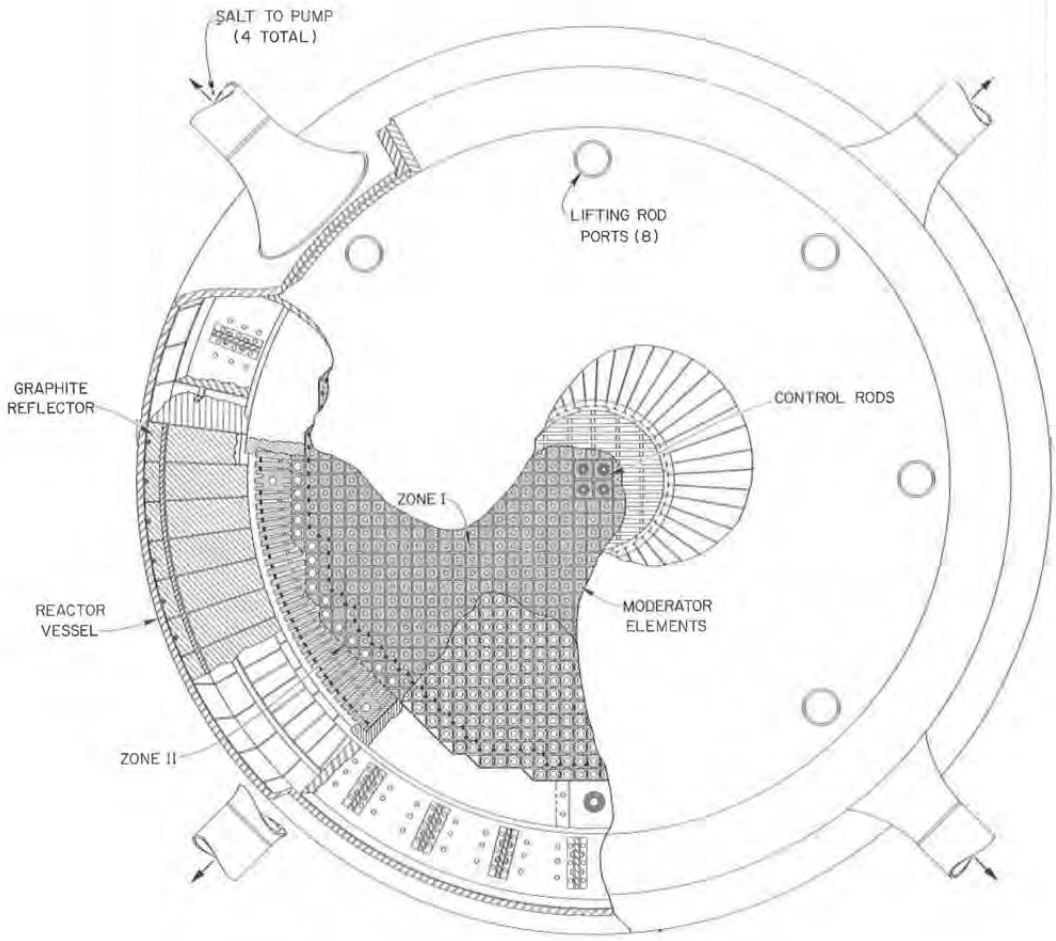
\includegraphics[width=\textwidth]{plan_view_vessel.png}
  \caption{Plan view of \gls{MSBR} vessel \cite{robertson_conceptual_1971}.}
  \vspace{-0.6em}
  \label{fig:ref_plan_msbr}
\end{figure}
\FloatBarrier

\begin{figure}[hbp!] % replace 't' with 'b' to 
  \centering
  \vspace{-0.3em}
  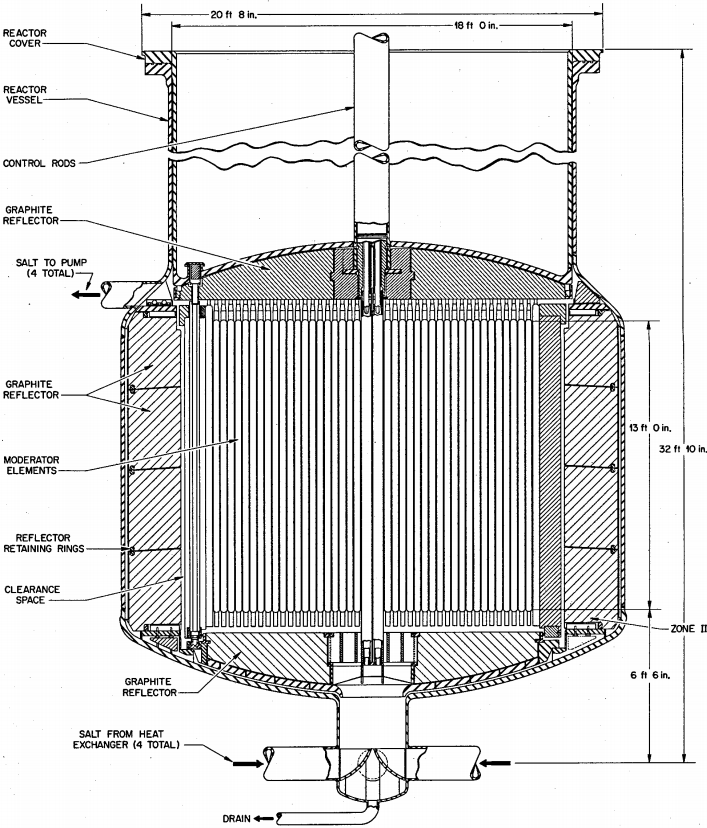
\includegraphics[width=\textwidth]{elev_view_vessel.png}
  \caption{Sectional elevation of \gls{MSBR} vessel \cite{robertson_conceptual_1971}.}
  \vspace{-0.6em}
  \label{fig:ref_sect_msbr}
\end{figure}
\FloatBarrier

There are eight graphite slabs with a width of 15.24 cm in zone II one to each other, one of which is illustrated in Fig.~\ref{fig:detail_plan_view}. The holes in the centers are for the core lifting rods used during the core replacement operations. These holes also allow a portion of the fuel salt to flow to the top of the vessel for cooling the top head and axial reflector. Fig.~\ref{fig:detail_plan_view} also demonstrates the 5.08-cm-wide annular space between the removable core graphite in zone II-B and the permanently mounted reflector graphite. This annulus, 100\% constists of fuel salt, provides space for moving the core assembly, helps compensate the out-of-roundness dimensions of the reactor vessel, and serves to reduce the damage flux at the surface of the graphite reflector blocks.

\begin{figure}[hbp!] % replace 't' with 'b' to 
  \centering
  \vspace{-0.3em}
  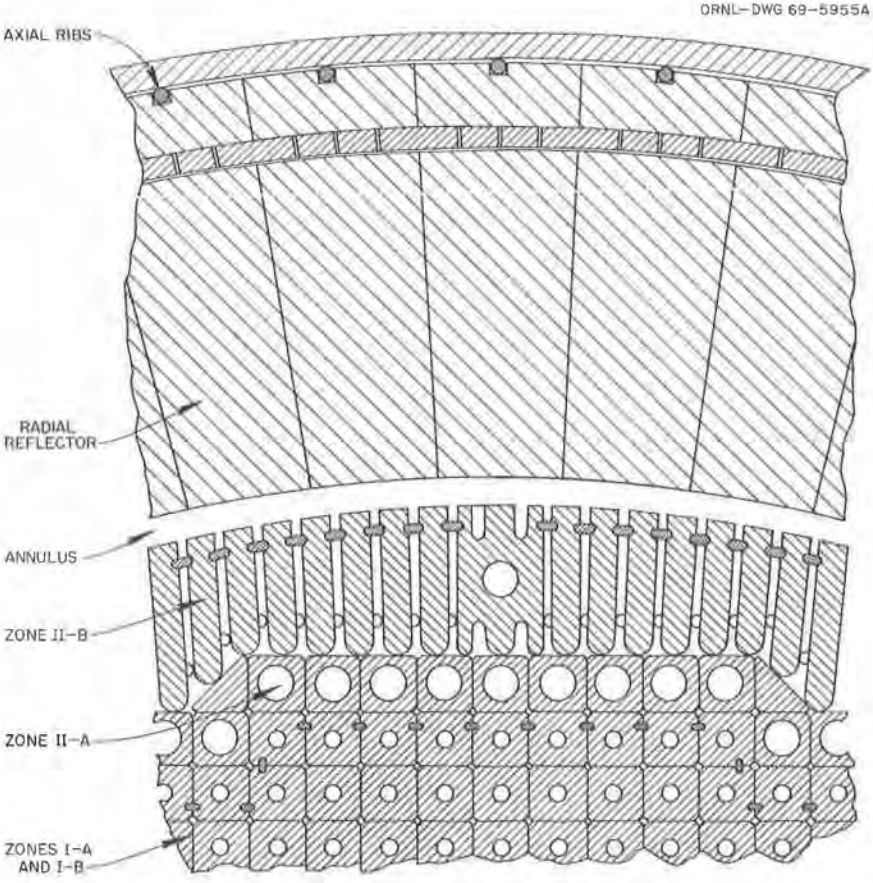
\includegraphics[width=\textwidth]{reflector_elements_ref.png}
  \caption{Detailed plan view of graphite reflector and moderator elements \cite{robertson_conceptual_1971}.}
  \vspace{-0.6em}
  \label{fig:detail_plan_view}
\end{figure}
\FloatBarrier

\subsection{Core zone I}
The central region of the core, called zone I, is made up of graphite elements, each $10.16$cm$\times$10.16cm$\times$396.24cm. In zone I, 13\% of the volume is fuel salt and 87\% is graphite. Zone I is composed of 1'320 graphite cells and 4 channels for control rods: two for graphite rods which both regulate and shim during normal operation, and two for backup safety rods consisting of boron carbide clad to assure sufficient negative reactivity for emergency situations.

These graphite elements have a mostly rectangular shape with lengthwise ridges at each corner that leave space for salt flow elements. Various element sizes reduce the peak damage flux and power density in the center of the core prevent local graphite damage. Zone I is well-moderated which is necessarily to achieve desired fission power density. Figure~\ref{fig:I_element_ref} demonstrates the elevation and sectional views of graphite elements of zone I \cite{robertson_conceptual_1971} and these elements SERPENT model \cite{rykhlevskii_full-core_2017}.

\subsection{Core zone II}
The undermoderated zone, zone II, surrounds zone I. Combined with the bounding radial reflector, zone II serves to diminish neutron leakage. This zone is formed of two kinds of elements: elements like those in zone I with a larger channel diameter (zone II-A), and radial graphite slats (zone II-B). 

Zone II has 37\% fuel salt by volume and each element has a fuel channel 
diameter of 6.604cm. It is divided into two different zones: zone II-A and zone 
II-B. The graphite elements for zone II-A are prismatic and have elliptical-shaped dowels running axially between the prisms and needed to isolate the fuel salt flow in zone I from that in zone II. Fig.~\ref{fig:II_element_ref} shows shape and dimensions of these graphite elements and their SERPENT model. Zone II-B elements are rectangular slats spaced far enough apart to provide the 0.37 fuel salt volume fraction. The reactor zone II-B graphite 5.08cm-thick slats vary in the radial dimension (average width is 26.67cm) as shown in figure~\ref{fig:detail_plan_view}. Zone II serves as ``blanket" to achieve the best ``performance" associated with a high breeding ratio and a low fissile inventory. The neutron energy spectrum in zone II is made harder, to enhance the rate of thorium resonance capture relative to the fission rate, thus limiting the neutron flux in the outer core zone and reducing the neutron leakage \cite{robertson_conceptual_1971}. 

\begin{figure}[hbp!] % replace 't' with 'b' to 
  \centering
  \vspace{-0.3em}
  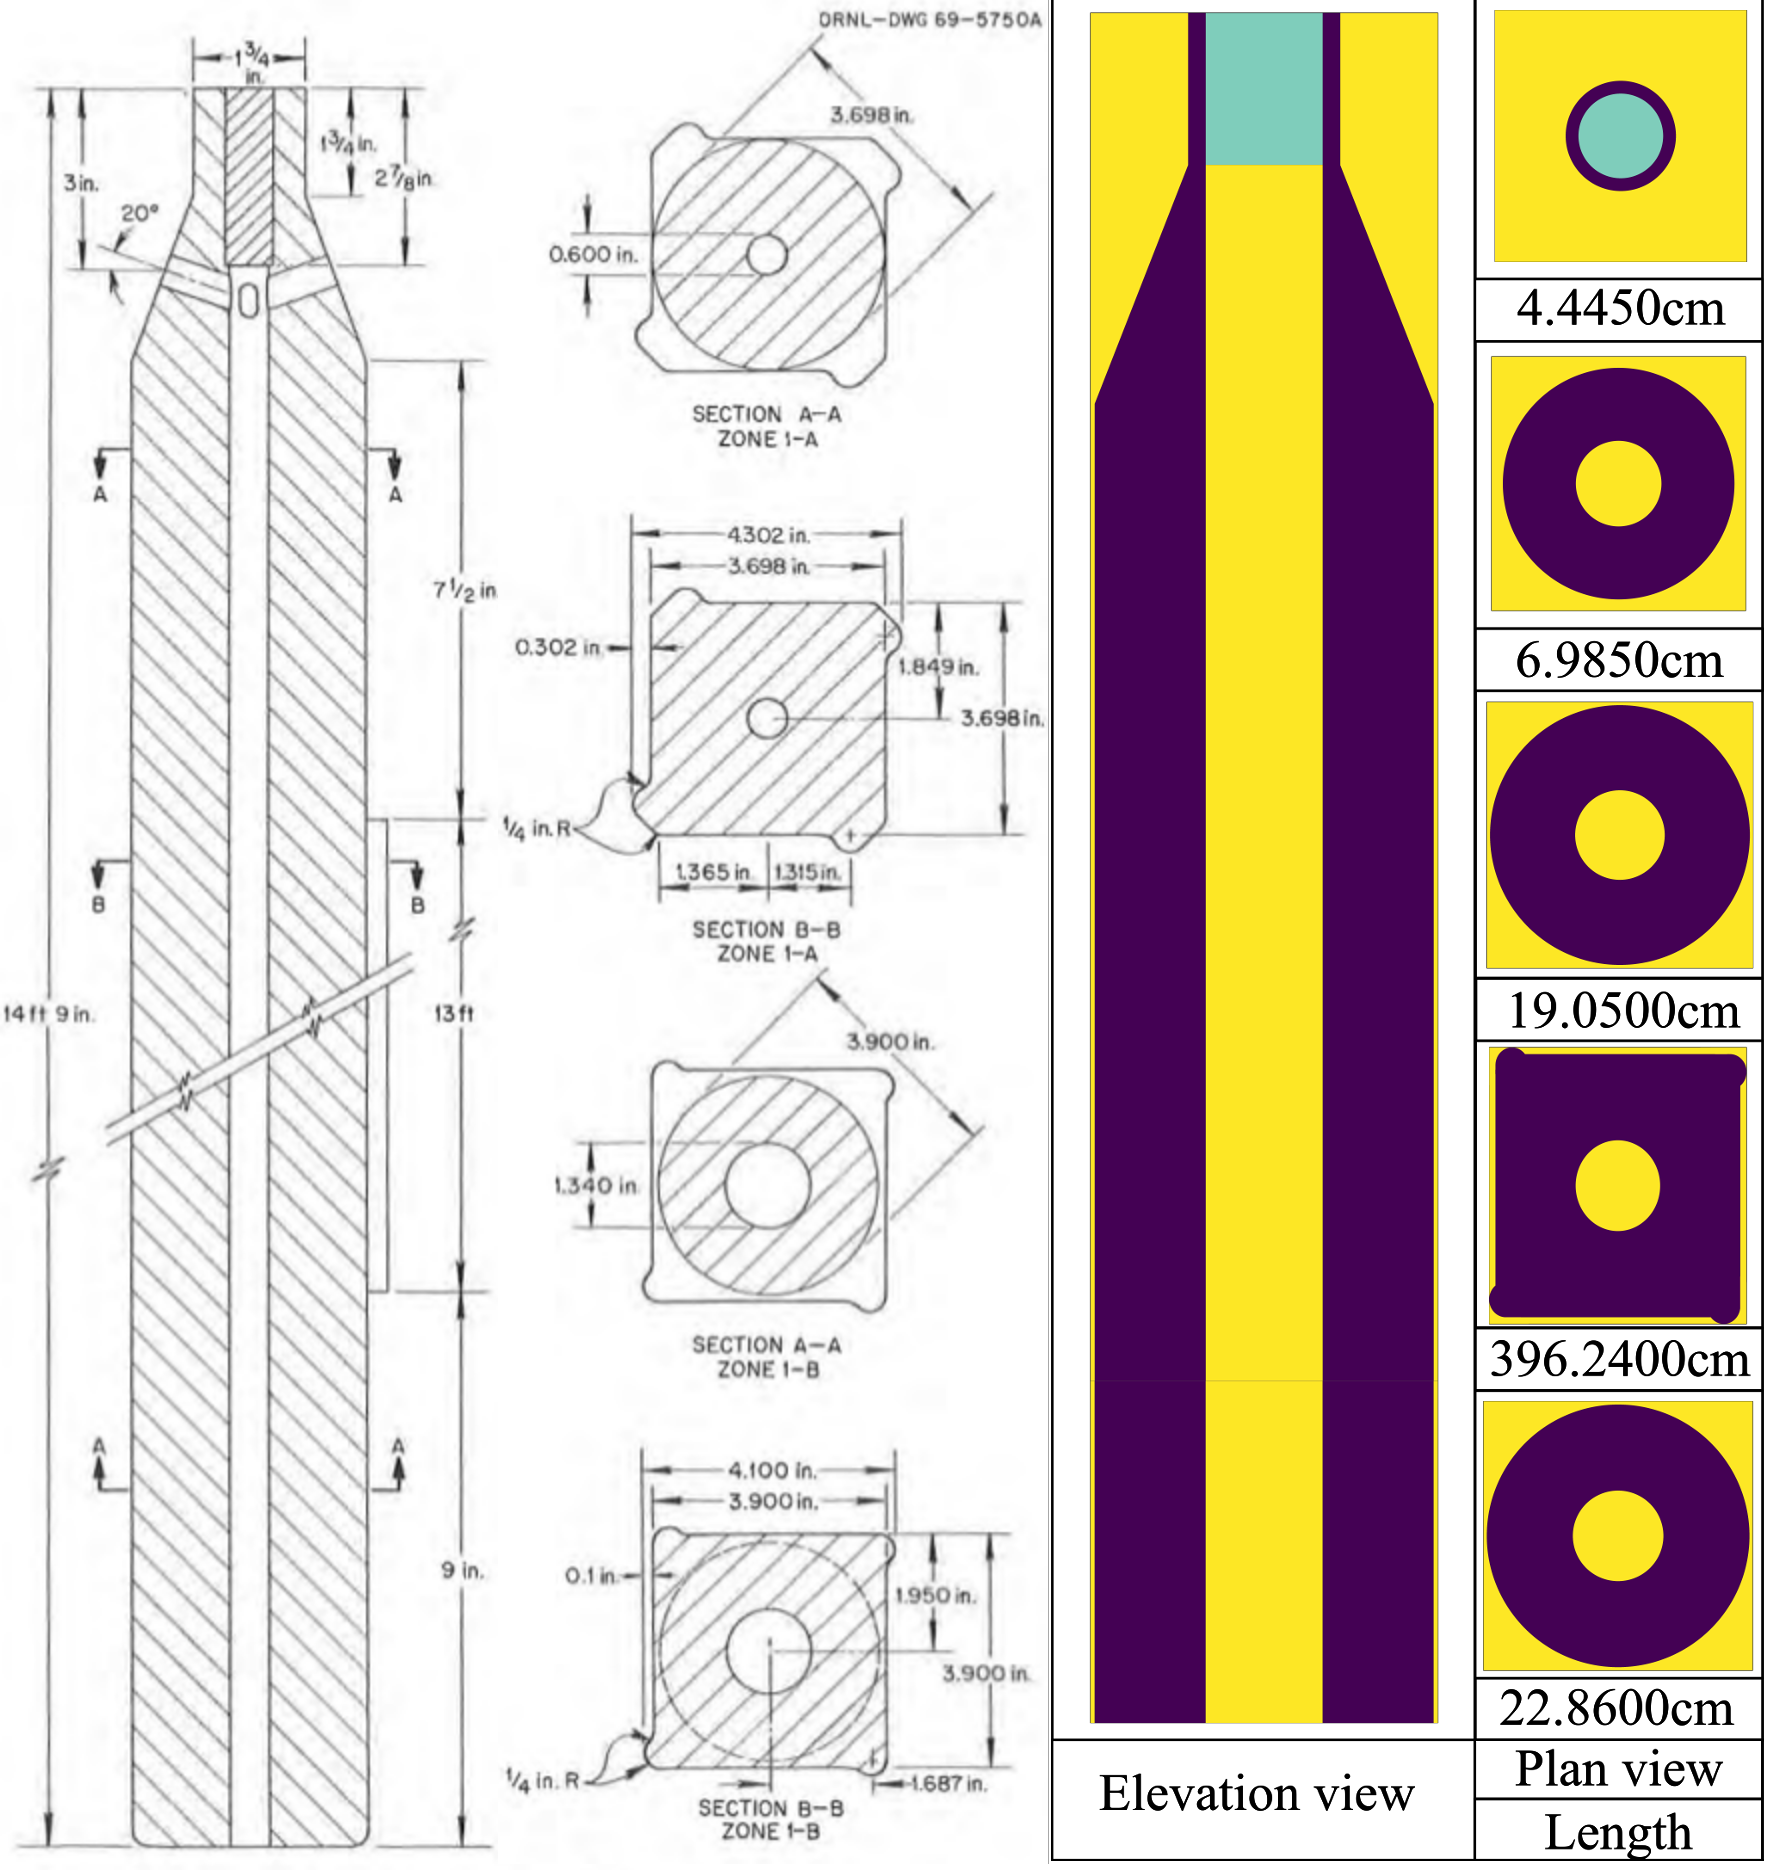
\includegraphics[width=1.04\textwidth]{zone_I_element_ref.png}
  \caption{Graphite moderator elements for zone I \cite{robertson_conceptual_1971,rykhlevskii_full-core_2017}.}
  \vspace{-0.6em}
  \label{fig:I_element_ref}
\end{figure}
\FloatBarrier

\begin{figure}[hbp!] % replace 't' with 'b' to 
  \centering
  \vspace{-0.3em}
  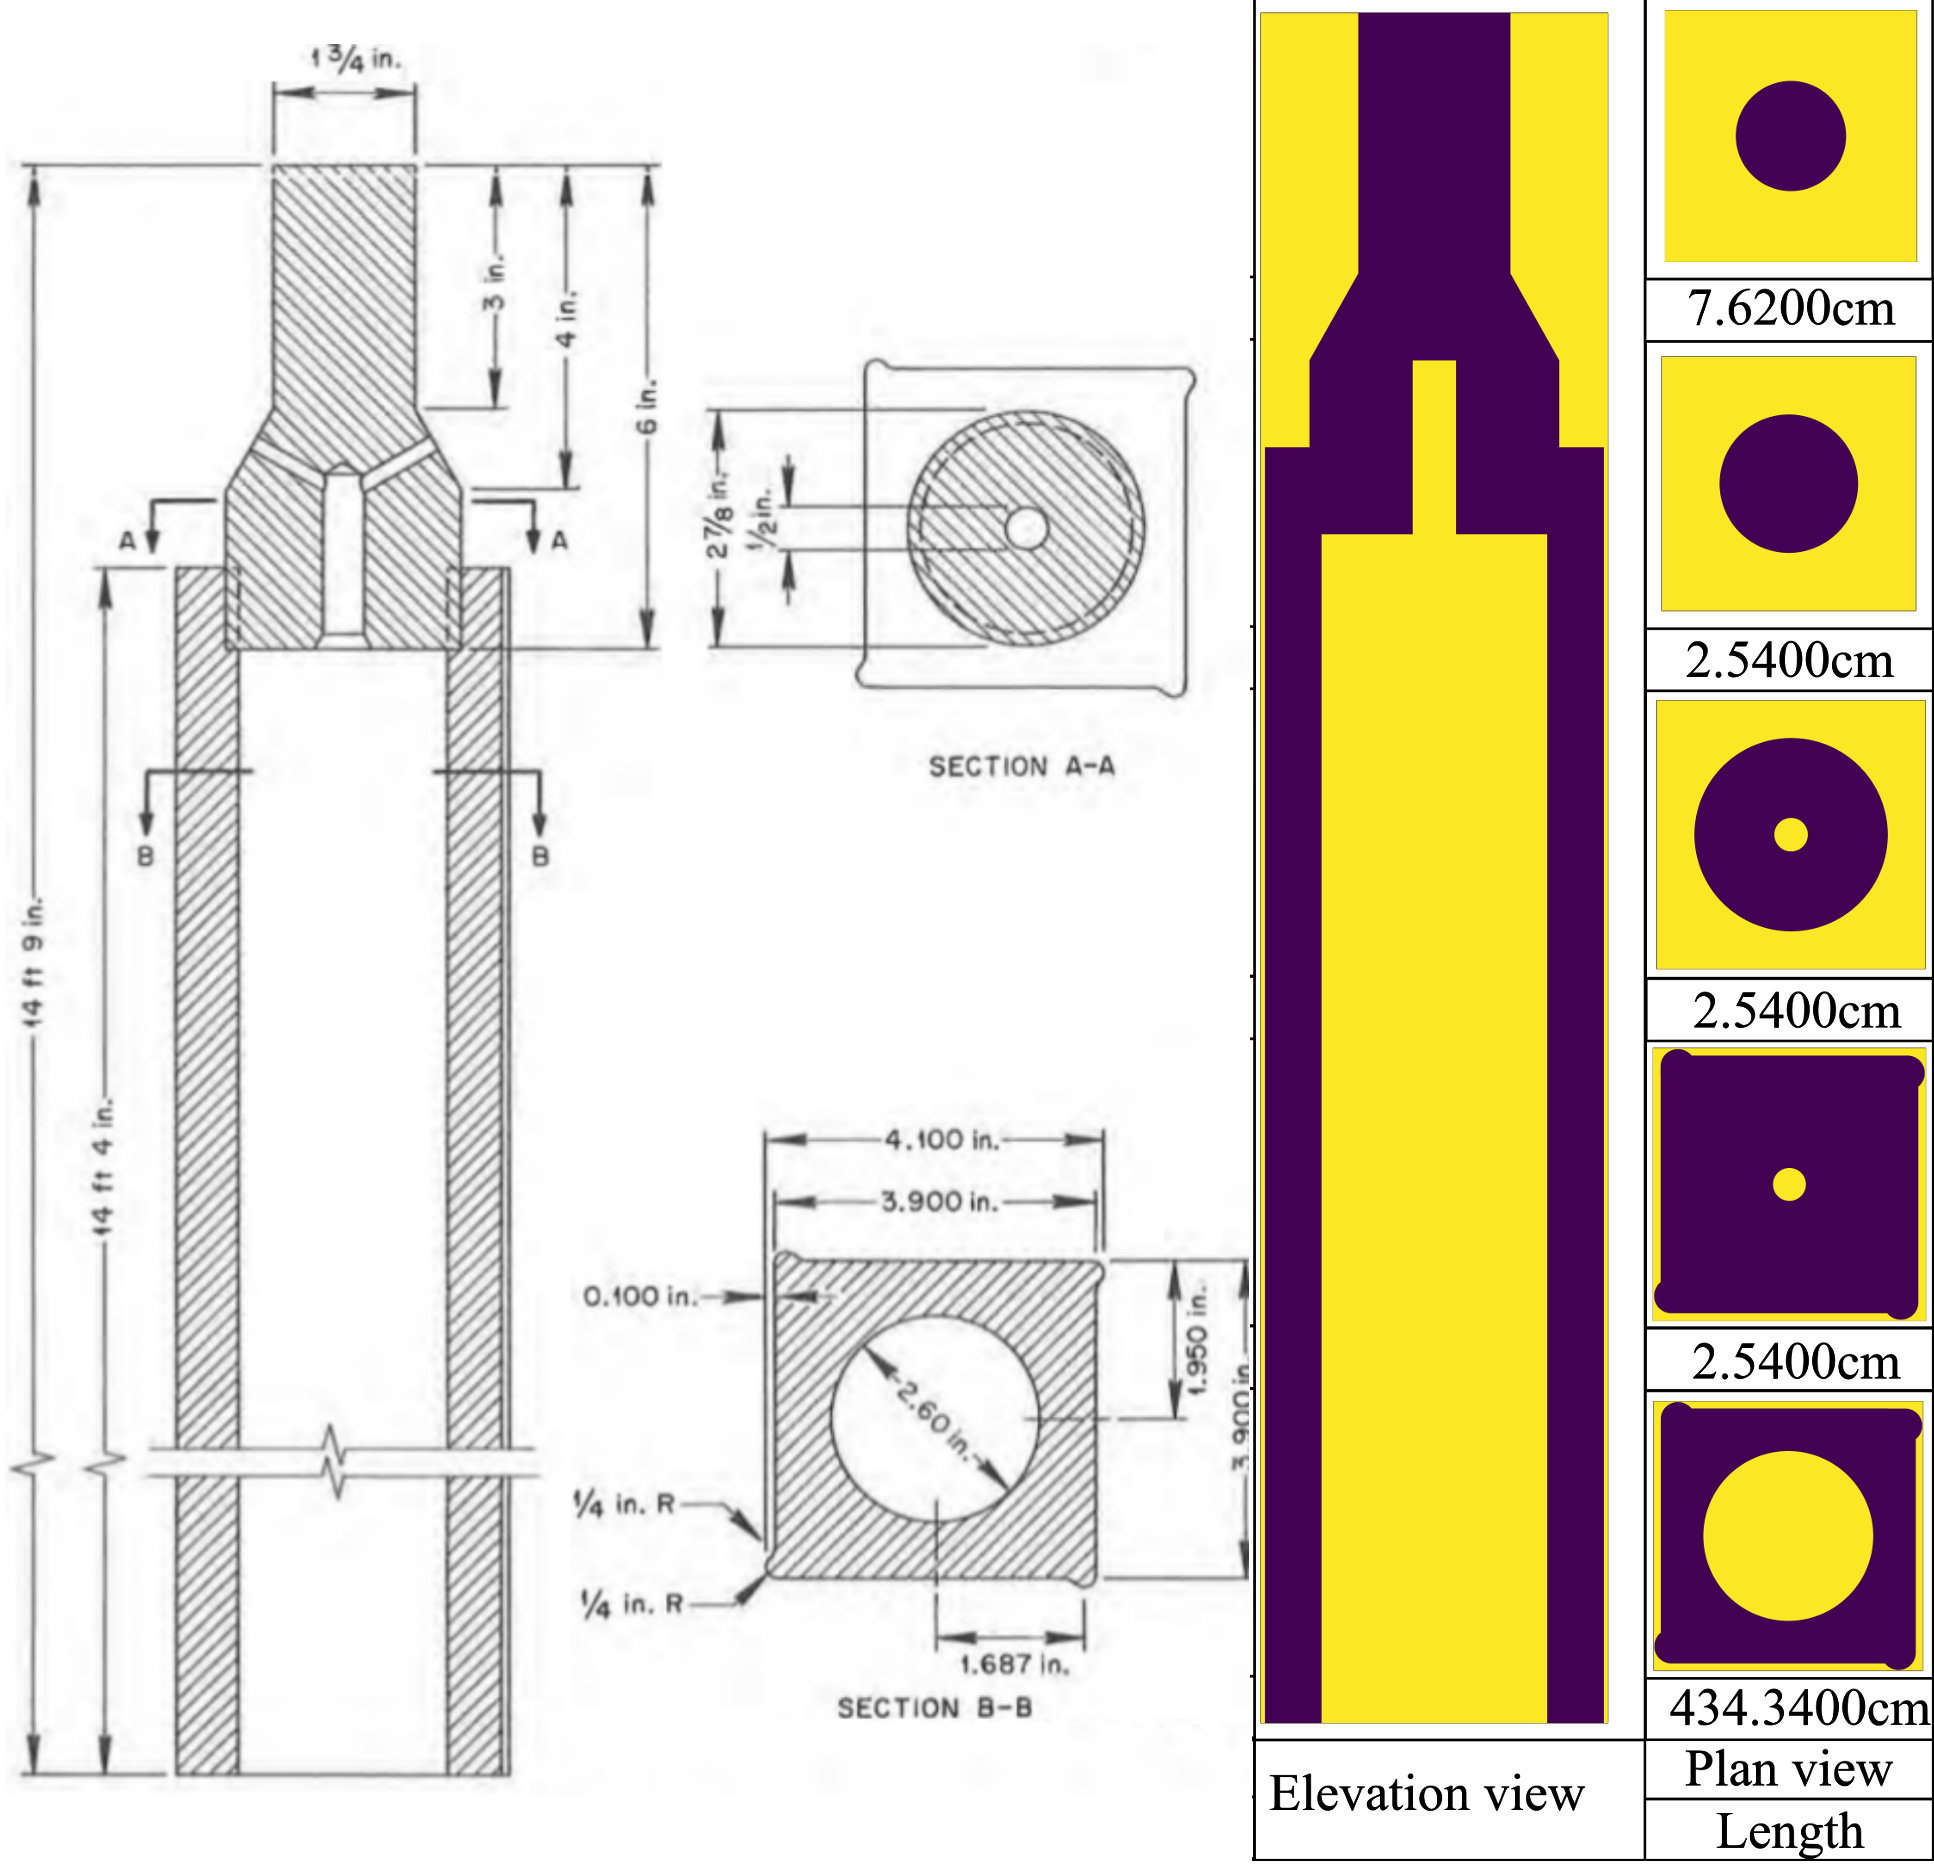
\includegraphics[width=1.04\textwidth]{zone_II_element_ref.png}
  \caption{Graphite moderator elements for zone II-A \cite{robertson_conceptual_1971,rykhlevskii_full-core_2017}.}
  \vspace{-0.6em}
  \label{fig:II_element_ref}
\end{figure}
\FloatBarrier

\section{Existing full-core MSBR models}
There are few recent studies presented full-core \gls{MSBR} models for neutronics analysis. First, MCNP6 model developed by Park \emph{et al.} for burn-up computations and safety parameters analysis \cite{park_whole_2015}. This model has significant simplifications in zone II-B graphite elements geometry, and completely ignore lengthwise ridges at each corner of cell. Figure~\ref{fig:park} shows simplifications in geometry of the model.  More recently Skirpan \emph{et al.} built a model of the core using Shift \cite{pandya_implementation_2016} to compare fidelity of one-cell, two-cell and full-core models of \gls{MSBR} \cite{skirpan_fuel_2017}. In this model complex cell geometry in zone I and zone II-A were approximated to sligtly rotated square cylinder (figure~\ref{fig:skirpan_cell}). Moreover, as can be seen from figure~\ref{fig:skirpan_plan}, zone II-B described using horizontal, vertical and 45$^\circ$-degree graphite elements, that might significantly distort neutron flux and reacton rates in that region, and, consequently, misrepresent breeding parameters of the whole reactor.

In sum: full-core Monte Carlo model with sufficient fidelity necessarily for online reprocessing and refueling simulation. Moreover, high-fidelity model essential for problem-oriented homogenized nuclear data (multi-group cross sections and diffusion constants) generation for deterministic reactor codes, and for coupled simulations.

\begin{figure}[hbp!] % replace 't' with 'b' to 
  \centering
  \vspace{-0.3em}
  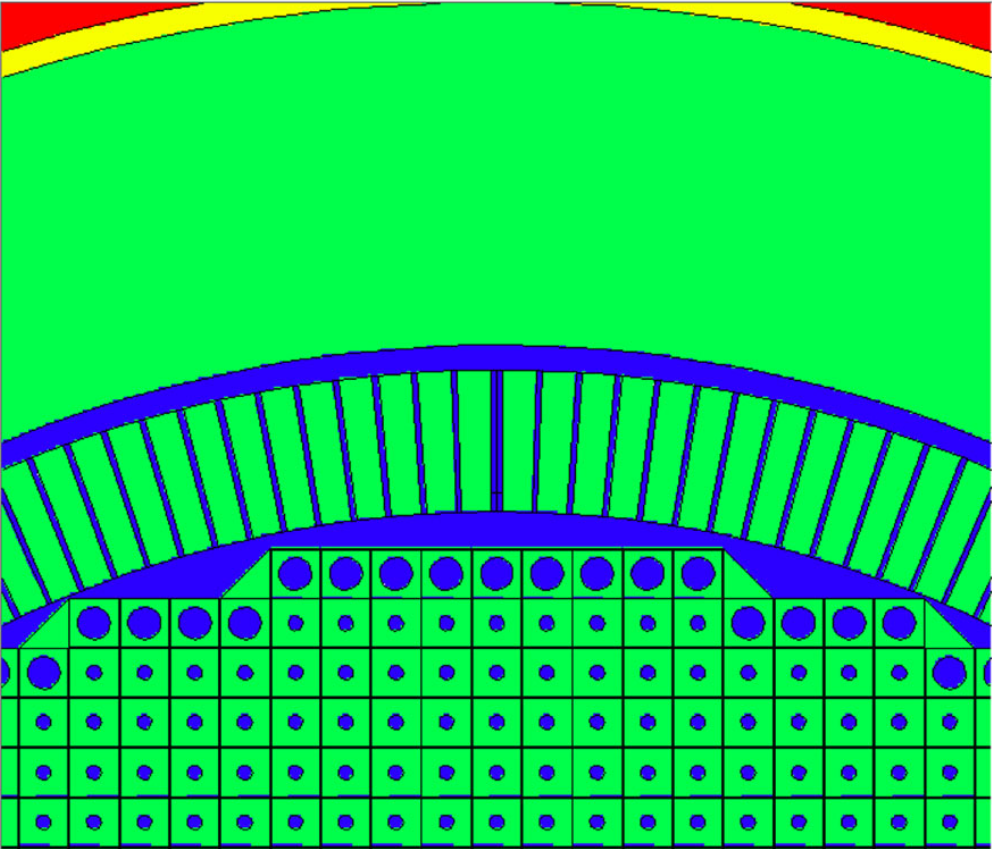
\includegraphics[width=\textwidth]{park_detailed_view.png}
  \caption{Graphite moderator elements  for zone II and reflector from Park \gls{MSBR} model (MCNP6) \cite{park_whole_2015}.}
  \vspace{-0.6em}
  \label{fig:park}
\end{figure}
\FloatBarrier

\begin{figure}[htp!] % replace 't' with 'b' to 
  \centering
  \vspace{-0.3em}
  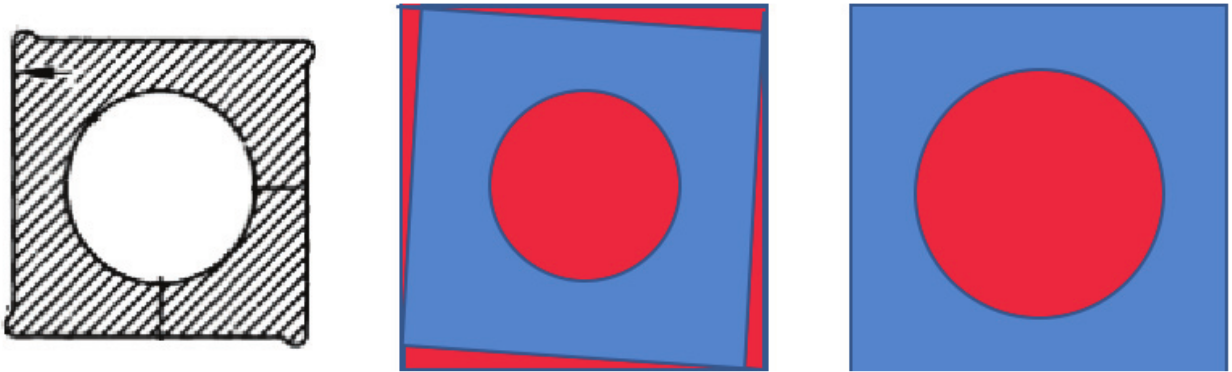
\includegraphics[width=0.95\textwidth]{skirpan_cell.png}
  \caption{Geometry of an MSBR fuel channel (left) approximated with a simple geometric model (center) to calculate appropriate volumes to reduce to a two-region model (right) \cite{skirpan_fuel_2017}.}
  \vspace{-0.6em}
  \label{fig:skirpan_cell}
\end{figure}

\begin{figure}[hbp!] % replace 't' with 'b' to 
  \centering
  \vspace{-0.3em}
  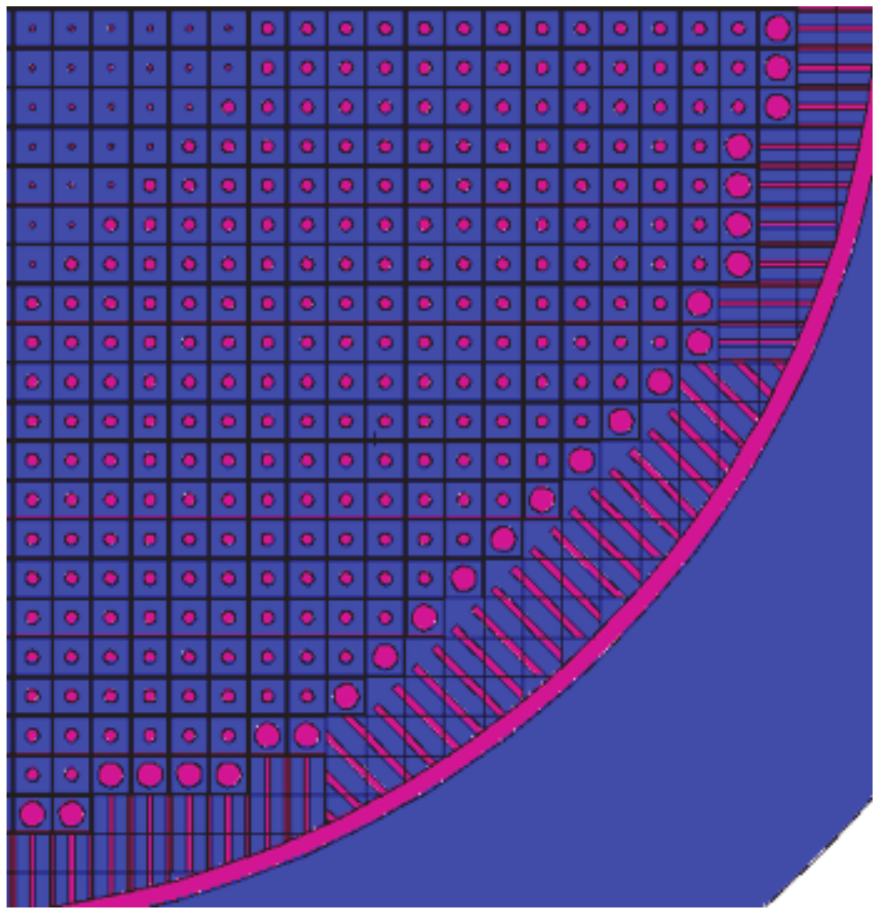
\includegraphics[width=0.7\textwidth]{skirpan_plan_view.png}
  \caption{Plan view of the \gls{MSBR} full-core transport model at core horizontal midplane \cite{skirpan_fuel_2017}.}
  \vspace{-0.6em}
  \label{fig:skirpan_plan}
\end{figure}
\FloatBarrier

\section{SERPENT 2 model}

To represent complex irregular \gls{MSBR} core geometry advanced geometry surfaces in SERPENT was employed. Fig.~\ref{fig:serpent_plan_view} shows the plan view of the whole-core configuration at the expected reactor operational level when both graphite control rods are fully inserted, and the safety rods are fully withdrawn. The safety rods only get inserted during an accident and were not considered in this model. Another feature of the \gls{MSBR}, its circulating liquid fuel and corresponding delayed neutron precursor drift, is not treated
here also. 

Fig.~\ref{fig:serpent_sectional_view} shows the longitudinal section of the reactor. The violet color represents bare graphite, and the yellow represents fuel salt. The blue color shows Hastelloy-N, a material used for the plenum and vessel wall, and the white color is a void space. The model contains about 2000 geometry surfaces and 2066 calculation zones. In this thesis, all figures of the core were generated using the built-in SERPENT plotter.

\begin{figure}[hbp!] % replace 't' with 'b' to 
  \centering
  \vspace{-0.3em}
  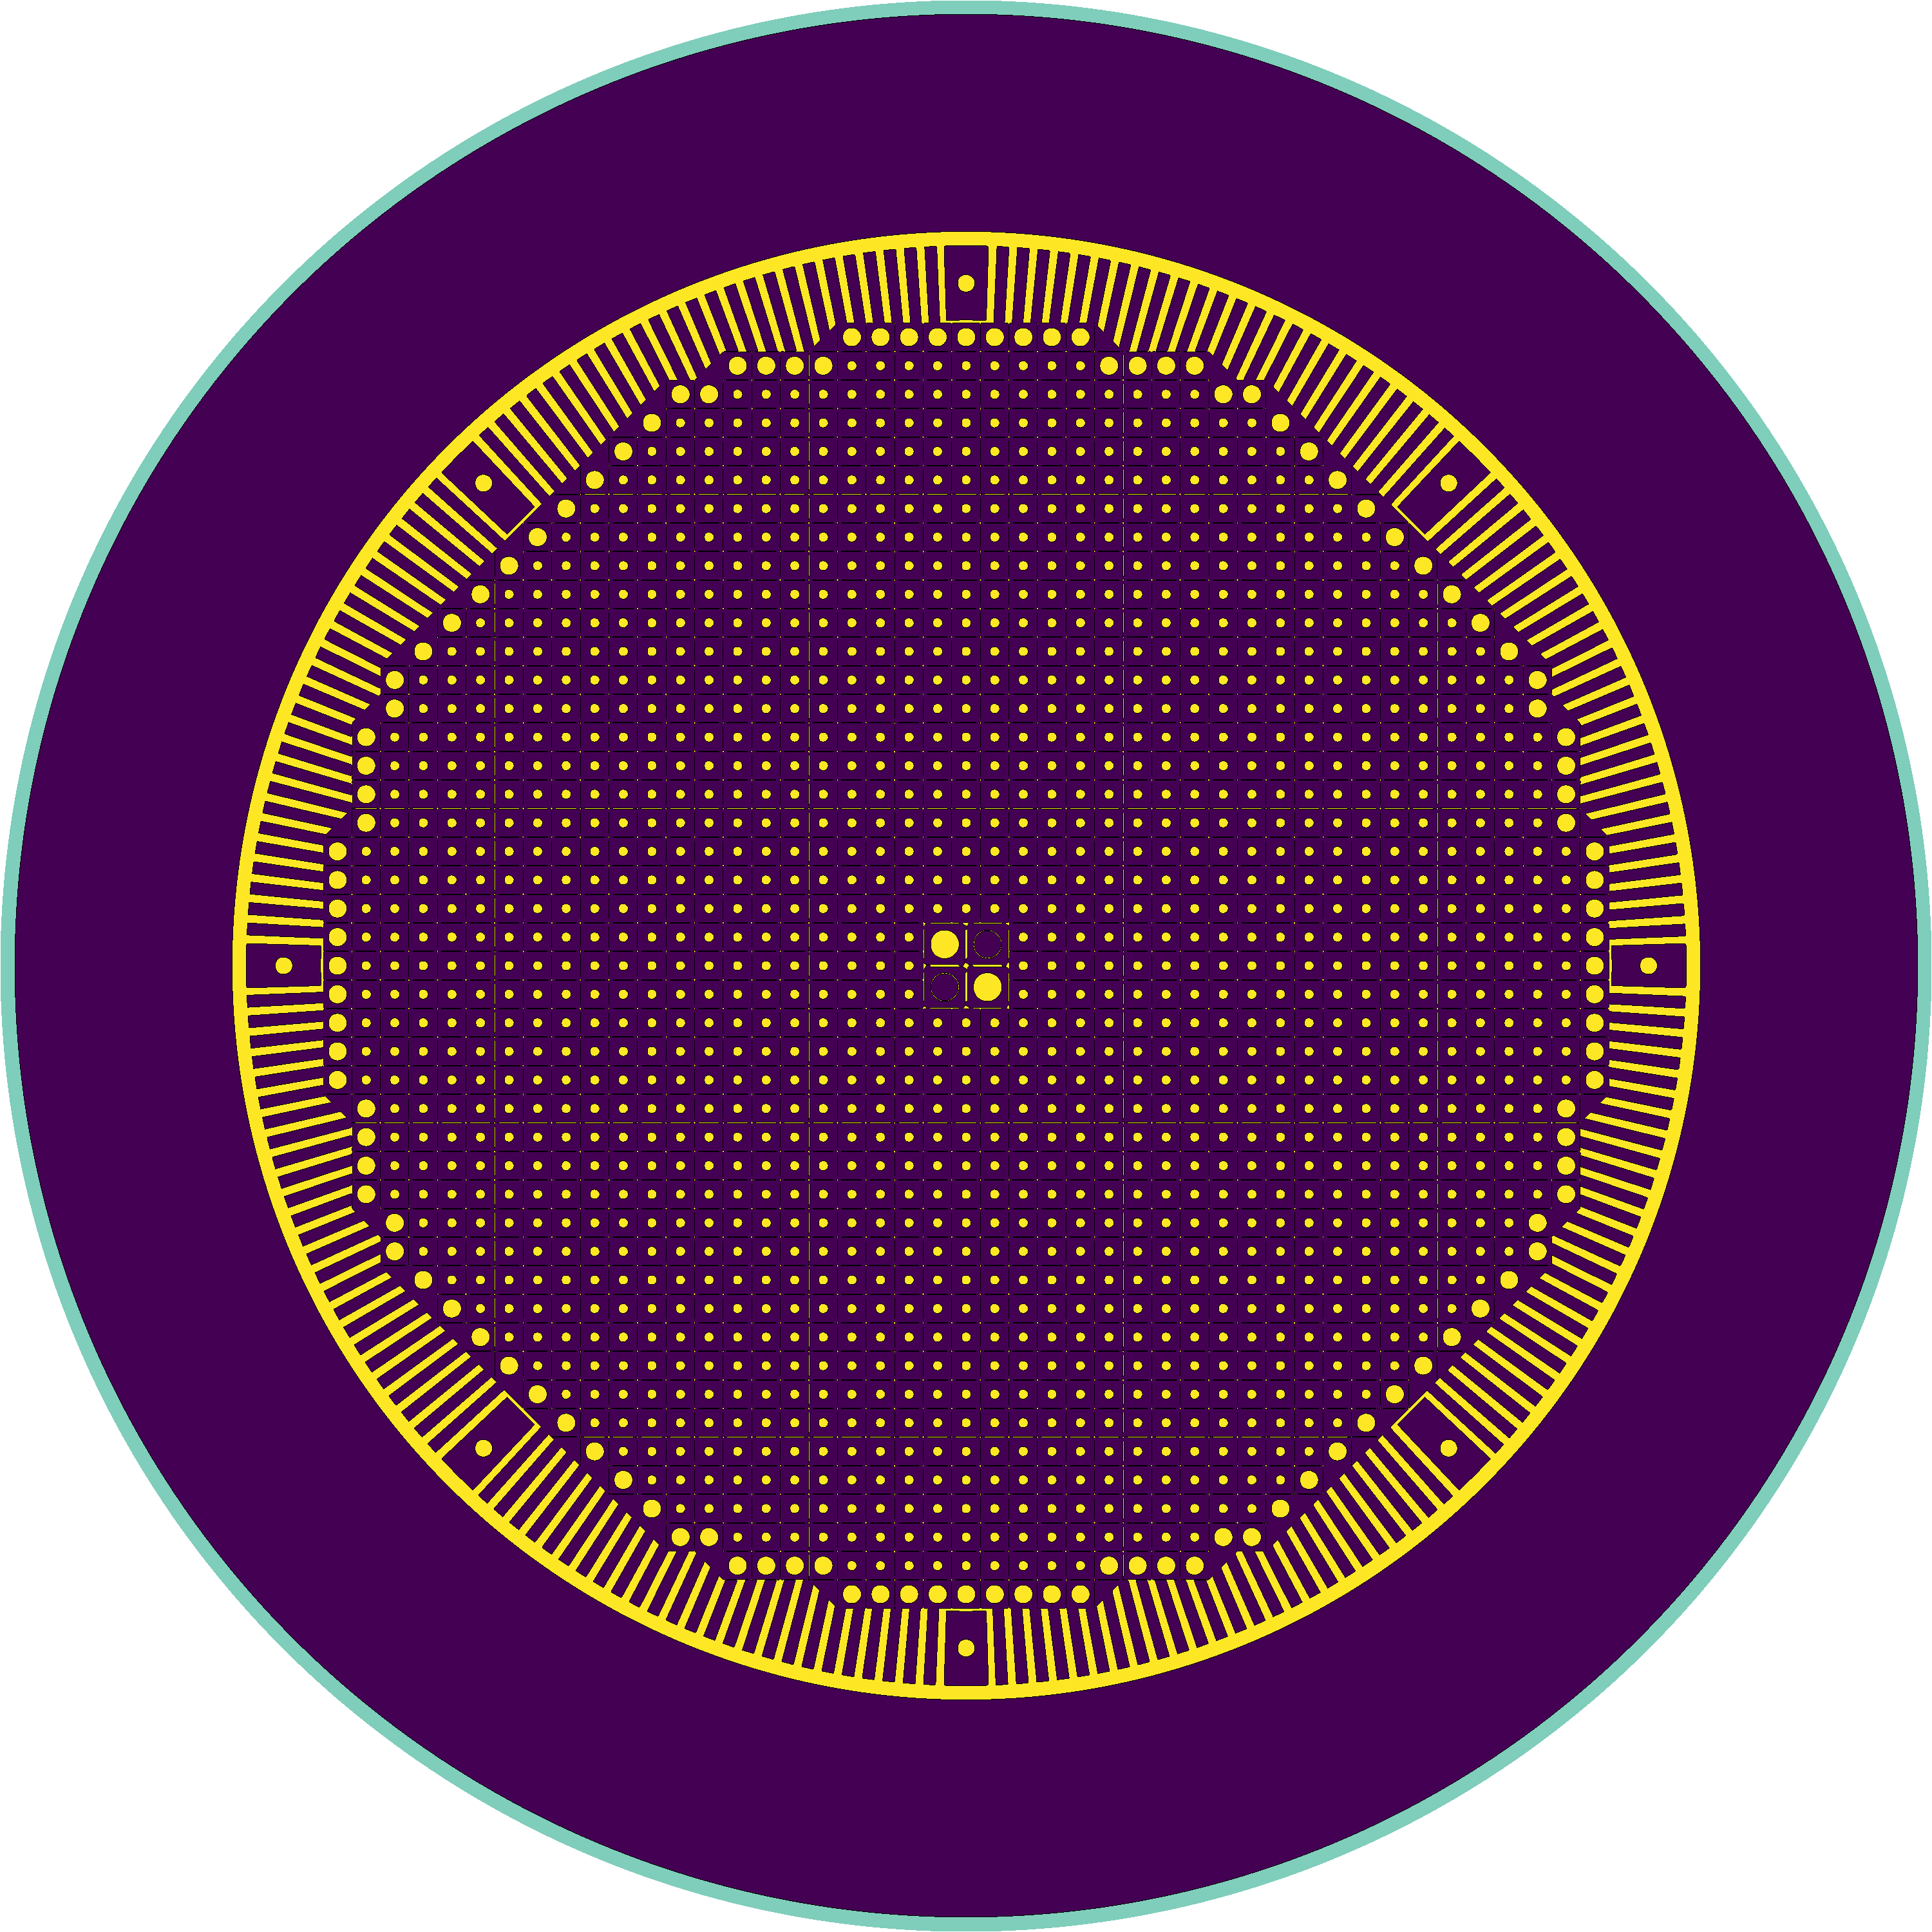
\includegraphics[width=1.05\textwidth]{plan_view_ser.png}
  \caption{Plan view of \gls{MSBR} model.}
  \vspace{-0.6em}
  \label{fig:serpent_plan_view}
\end{figure}
\FloatBarrier

\begin{figure}[hbp!] % replace 't' with 'b' to 
  \centering
  \vspace{-0.3em}
  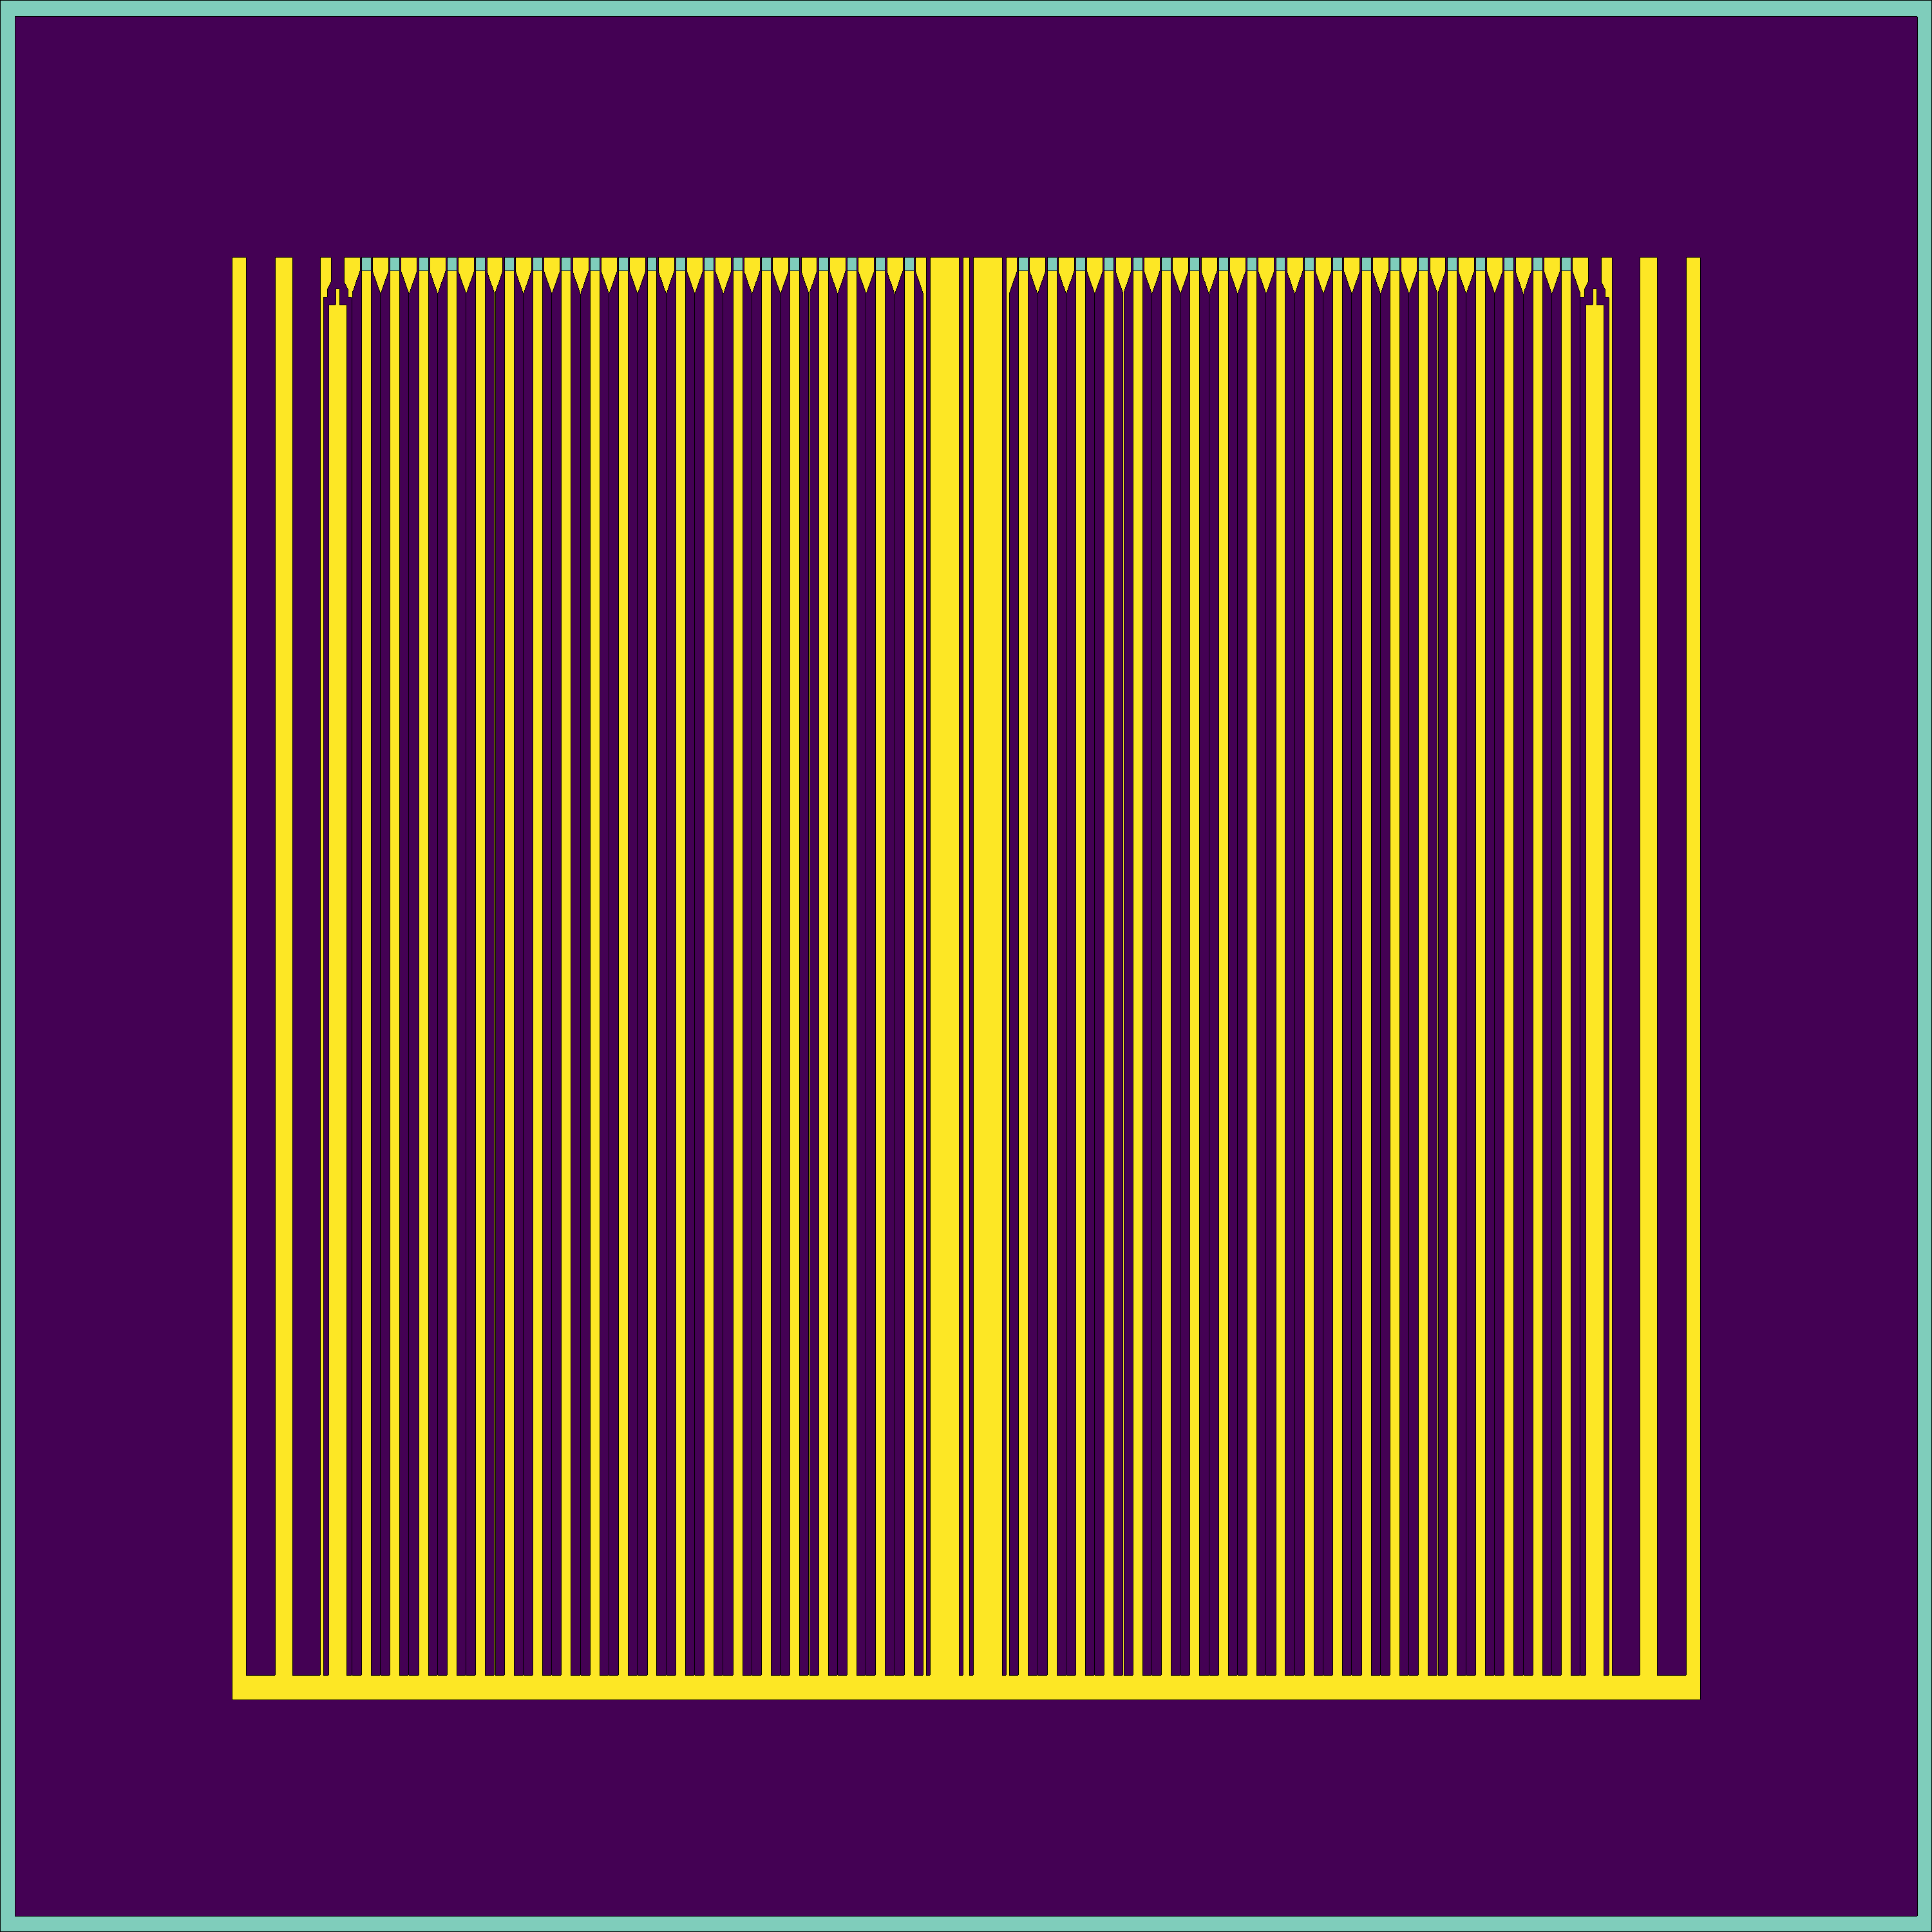
\includegraphics[width=1.05\textwidth]{sect_view_ser.png}
  \caption{Elevation view of \gls{MSBR} model.}
  \vspace{-0.6em}
  \label{fig:serpent_sectional_view}
\end{figure}
\FloatBarrier

In the model, zone I, zone II-A graphite blocks was described using circular cylinder and square cylinder surface types, lengthwise ridges at each corner mentioned earlier was specified using dodecagonal cylinder surfaces and general planes (figure~\ref{fig:I_element_ref}, \ref{fig:II_element_ref}). Zone I of the core was described using square lattice inscribed in the octagonal cylinder surfaces to accurately represent geometry of that region.

The main challenge was accurately represent zone II-B because it has irregular elements with sophisticated shape. From the \gls{ORNL} report \cite{robertson_conceptual_1971}, the suggested design of zone II-B has 8 irregularly-shaped graphite elements every 45$^\circ$ as well as salt channels (figure~\ref{fig:detail_plan_view}). These graphite elements were simplified into right-circular cylindrical shapes  with central channels. Fig.~\ref{fig:serpent_zoneII} illustrates this core region in SERPENT model. Volume of fuel salt in zone II kept exactly 37\%, consequently, this simplification did not considerably change neutronics of the core. This is the only simplification made to the \gls{MSBR} conceptual geometry in this work. 

\begin{figure}[hbp!] % replace 't' with 'b' to 
  \centering
  \vspace{-0.3em}
  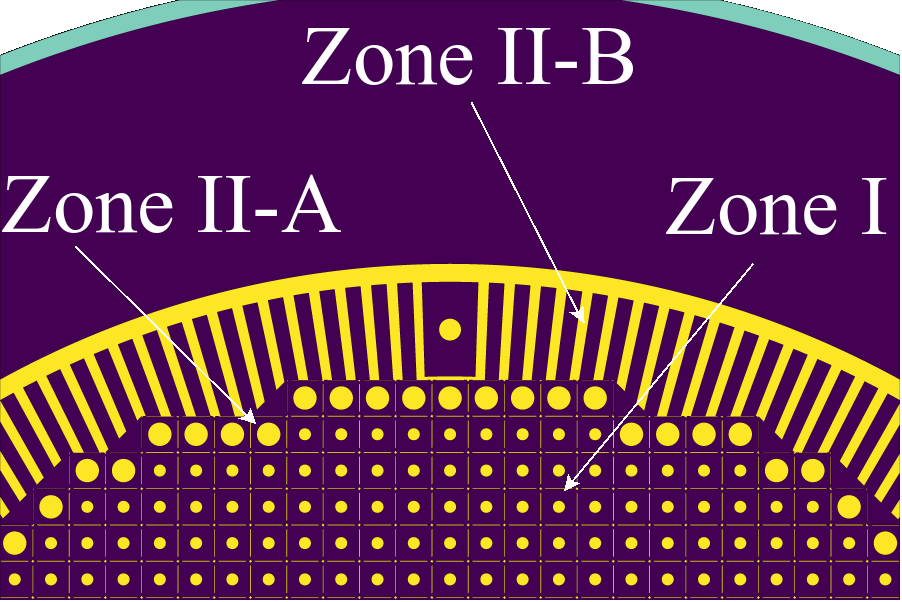
\includegraphics[width=1.05\textwidth]{ser_zone_II.png}
  \caption{Detailed view of \gls{MSBR} zone II model.}
  \vspace{-0.6em}
  \label{fig:serpent_zoneII}
\end{figure}
\FloatBarrier

\subsection{Material composition and normalization parameters}
The fuel salt, the reactor graphite, and the modified Hastelloy-N are materials 
unique of the \gls{MSBR} and were created at \gls{ORNL}. The initial fuel salt used the same density (3.35 g/cm$^3$) and composition LiF-BeF$_2$-ThF$_4$-$^{233}$UF$_4$ (71.8-16-12-0.2 mole \%) as the \gls{MSBR} design\cite{robertson_conceptual_1971}. The lithium in the molten salt fuel is a fully enriched $^{7}$Li because $^{6}$Li is a very strong neutron poison and becomes tritium upon neutron capture. 

For cross section generation, JEFF-3.1.2 was employed \cite{oecd/nea_data_bank_jeff-3.1.2_2014}. The specific temperature was fixed for each material to correctly model the Doppler-broadening of resonance peaks when Serpent generate problem-oriented nuclear data library. The isotope composition of each material at the initial state was described in detail in the MSBR conceptual design study \cite{robertson_conceptual_1971} and has been applied to Serpent model without any modification. Table~\ref{tab:msbr_tab} is the summary of the major \gls{MSBR} parameters used by this model \cite{robertson_conceptual_1971}. 

%%%%%%%%%%%%%%%%%%%%%%%%%%%%%%%%%%%%%%%%
\begin{table}[h!]
        %\centering
        \caption{Summary of principal data for MSBR \cite{robertson_conceptual_1971}.}
        \begin{tabular}{|m{0.56\linewidth} | m{0.40\linewidth}|}
        \hline [5pt]
        %\begin{tabularx}{\linewidth}{l X} \toprule 
                Thermal capacity of reactor           & 2250 MW(t)
                \\ [5pt] \hline 
                Net electrical output                 & 1000 MW(e) 
                \\ [5pt] \hline 
                Net thermal efficiency        & 44.4\%
                \\ [5pt] \hline 
                Salt volume fraction in central core zone     & 0.13
                \\ [5pt] \hline 
                Salt volume fraction in outer core zone       & 0.37
                \\ [5pt] \hline 
                Fuel salt inventory (Zone I)                  & 8.2 m$^3$	
                \\ [5pt] \hline 
                Fuel salt inventory (Zone II)                 & 10.8 m$^3$	
                \\ [5pt] \hline 
                Fuel salt inventory (annulus)                 & 3.8 m$^3$	
                \\ [5pt] \hline 
                Total fuel salt inventory                     & 48.7 m$^3$	
                \\ [5pt] \hline 
                Fissile mass in fuel salt                   & 1303.7 kg	
                \\ [5pt] \hline 
                Fuel salt components                  & 
                LiF-BeF$_2$-ThF$_4$-$^{233}$UF$_4$	
                \\ [5pt] \hline 
                Fuel salt composition                 & 
                71.9-16-12-0.2 mole\%
                \\[5pt]  \hline 
                Fuel salt density                    & 
                3.35 g/cm$^3$
                \\[5pt]  \hline 
        \end{tabular}
        \label{tab:msbr_tab}
\end{table}
%%%%%%%%%%%%%%%%%%%%%%%%%%%%%%%%%%%%%%%%%%%%%%%%


\chapter[Online reprocessing simulation]{Online reprocessing simulation}

\section{Online reprocessing method}

\section{Python code description}

\section{Results and equilibrium state analysis}
\chapter[Online reprocessing simulation]{Online reprocessing simulation}

\section{Fuel salt processing systems}
Removing specific chemical elements from a molten salt is a complicated task that requires intelligent design (e.g., chemical separations equipment design, fuel salt flows to equipment) and has a considerable economic cost. This section contains \gls{MSBR} chemical processing plant and gas separation system brief overview.

\subsection{Fuel salt chemical processing facility}
All liquid-fueled \gls{MSR} designs involve varying levels of online fuel processing. Minimally, volatile gaseous fission products (e.g. Kr, Xe) escape from the fuel salt during routine reactor operation and must be captured. Additional systems might be used to intensify removal of those elements. Most designs also call for the removal of rare earth metals from the core since these metals act as neutron poisons. Some designs suggest a more complex list of elements to process (figure ~\ref{fig:periodic_tab}), including the temporary removal of protactinium from the salt or other regulation of the actinide inventory in the fuel salt \cite{ahmad_neutronics_2015}.

\begin{figure}[htp!] % replace 't' with 'b' to 
  \centering
  \vspace{-0.3em}
  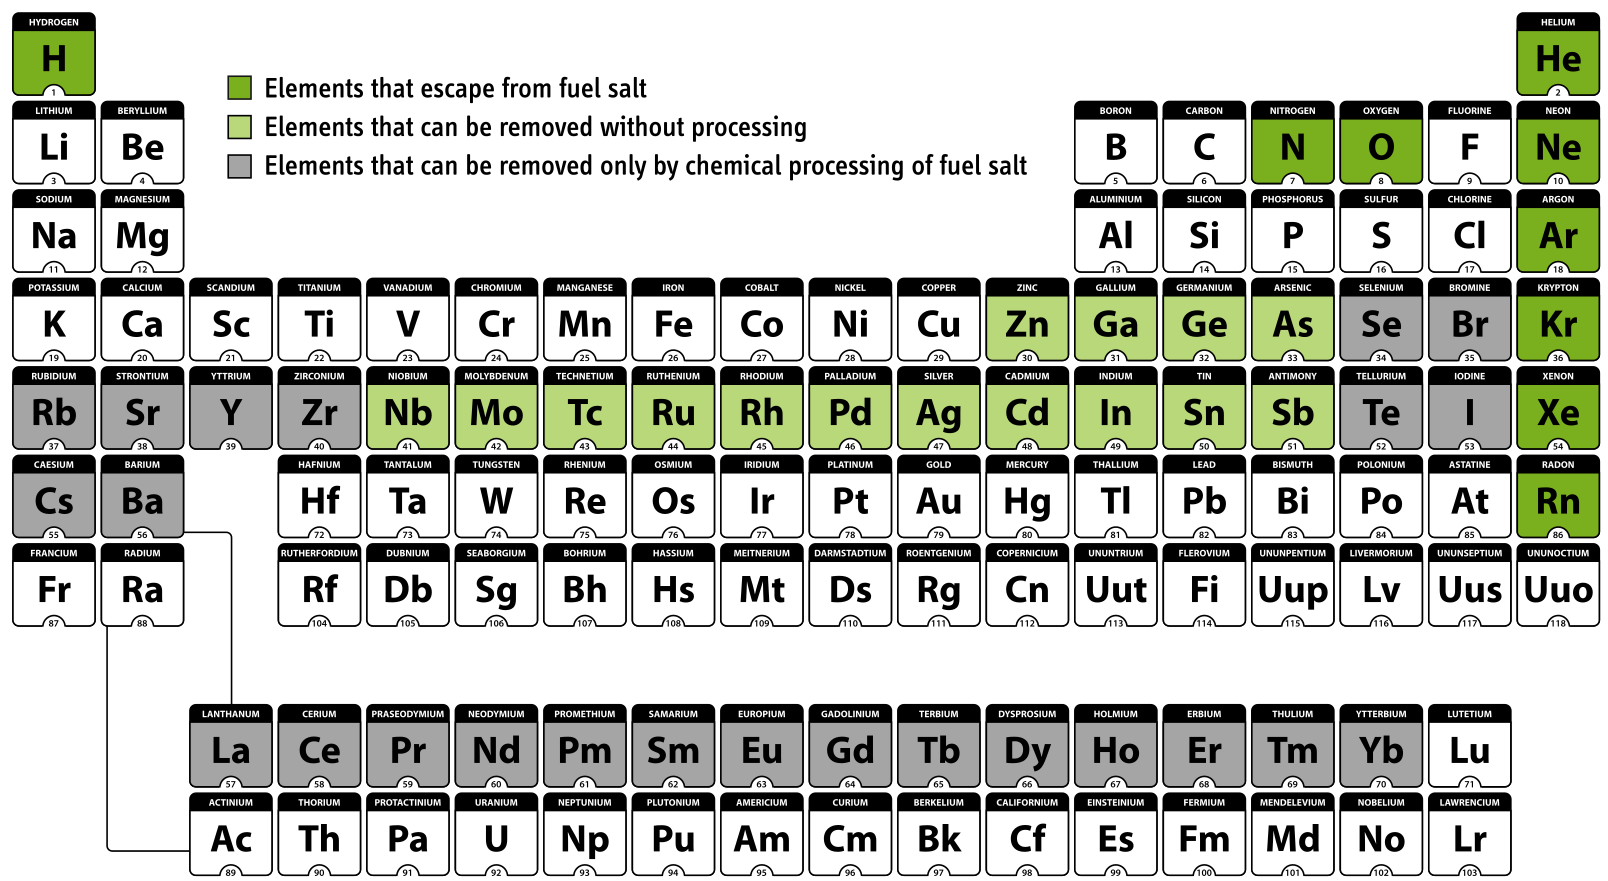
\includegraphics[width=1.05\textwidth]{periodic_map.png}
  \caption{Processing options for \gls{MSR} fuels \cite{ahmad_neutronics_2015}.}
  \vspace{-0.6em}
  \label{fig:periodic_tab}
\end{figure}
\FloatBarrier

In the single-fluid \gls{MSBR} considered in this work, thorium, uranium, protactinium, and fission products are all mixed together in a single fluoride salt (FLiBe). Separation of thorium from lanthanide (atomic numbers 57 through 71) fission products is rather challenging because of their chemical similarities. 

The principal scheme of \gls{MSBR} reprocessing facility concept is shown in Figure~\ref{fig:material_flow}. The fuel salt is first temporarily stored for cooling and decay of the shortest lived fission products, then directed to the primary fluorinator, where most of the uranium is removed by fluorination to UF$_6$. After that the salt is routed to an extraction column where mixture containing metallic bismuth, lithium and thorium as reductants are contacted with the salt. The remaining uranium and protactinium are reductively extracted to the bismuth, leaving a salt that only contains fission products dissolved in carrier salt (base composition of LiF-BeF$_2$-ThF$_4$).The salt then goes through a reduction column where UF$_6$ is reduced to UF$_4$ in the salt, refueling it and preparing it for return to the reactor. Refill BeF$_2$ and ThF$_4$ are also added and all residual bismuth is removed from the salt. After a final cleanup step and valence adjustment the purified salt returns to the reactor \cite{carter_design_1972,noauthor_one-fluid_nodate}.

The bismuth accommodating some uranium and protactinium is routed to a hydrofluorination column where the metallic solutes in the bismuth are oxidized into their fluoride forms in the presence of a decay salt. The decay salt, containing UF$_4$, PaF$_4$, and ThF$_4$ passes into a decay tank where $^{233}$Pa is decaysto $^{233}$U. This uranium generated by protactinium decay is removed through fluorination to UF$_6$ and directed to the reduction column to refuel the purified fuel salt. A hydrofluorinator and a fluorinator can remove approximately \textbf{95\%} of the uranium from the stream.

The fully processed salt, on its way back to the reactor, has uranium added from the protactinium decay tank at the rate required to maintain or adjust the uranium concentration in the reactor (and, consequently, control the reactivity). This is performed by sparging the salt with UF$_6$ and hydrogen to produce UF$_4$ in the salt and HF gas \cite{robertson_conceptual_1971}.

\begin{figure}[htp!] % replace 't' with 'b' to 
  \centering
  \vspace{-0.3em}
  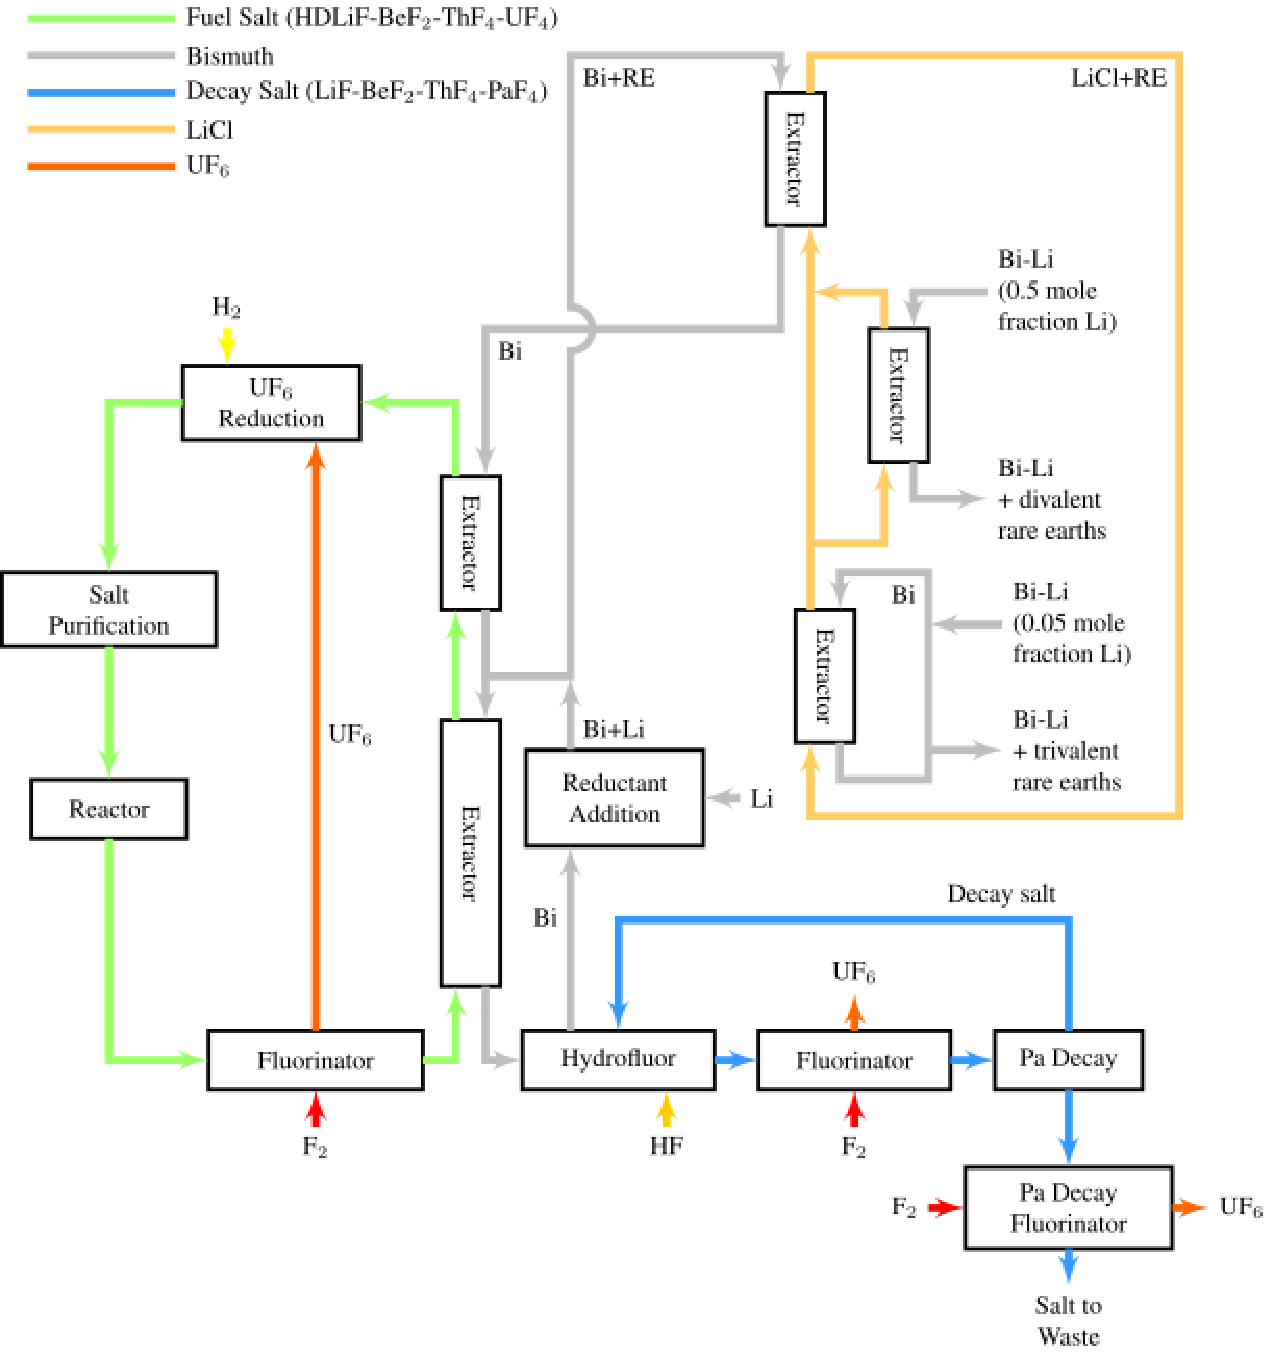
\includegraphics[width=1.05\textwidth]{flowsheet.pdf}
  \caption{Detailed block diagram of chemical processing scheme for single-fluid \gls{MSBR} \cite{robertson_conceptual_1971, noauthor_one-fluid_nodate}.}
  \vspace{-0.6em}
  \label{fig:material_flow}
\end{figure}
\FloatBarrier

\subsection{Gas separation system}
Volatile gaseous fission products (e.g. Kr, Xe) must be removed from the fuel salt to avoid reactor poisoning especially during starup and maneuvering. This is particularly true for $^{135}$Xe, with its very large absorption cross section. Tritium, xenon, and krypton are sparged from the fuel salt by helium introduced in a bypass stream by a bubble generator and subsequently removed by a gas separator. Indeed, noble gases, because of their exceptional insolubility in the salt, will migrate promptly to any gaseous interface available. Because they ideal-dilute solution in salt (obey Henry's law), they will migrate in accordance with the conventional laws of mass transfer. If tiny helium bubbles are circulated with the fuel salt, they will absorb xenon and krypton fission products. The fission-product-rich bubbles of helium may then be separated from the salt and discharged to the off-gas system. Xenon migration to the circulating bubbles is in competition with xenon migration to the porous moderator graphite. The graphite is especially of concern because it absorbs xenon and holds it in the core which leads to parasitic neutron absorption. In \gls{ORNL} report \cite{robertson_conceptual_1971} in Appendix A it is concluded that, with moderate success of the coated-graphite program, the 0.5\% target value for $^{135}$Xe poison fraction can be achieved when circulating helium bubbles 0.508mm in diameter. This is accomplished by bypassing 10\% of the fuel salt from
the pump discharge through a bubble separator to remove the xenon bubbles, then through a clean helium bubble generator for replenishment of helium bubbles, and back into the pump suction, as shown in Figure~\ref{fig:gas_removal_system}. The average residence time of a bubble in the fuel loop would be 10 full cycles.

\begin{figure}[htp!] % replace 't' with 'b' to 
  \centering
  \vspace{-0.3em}
  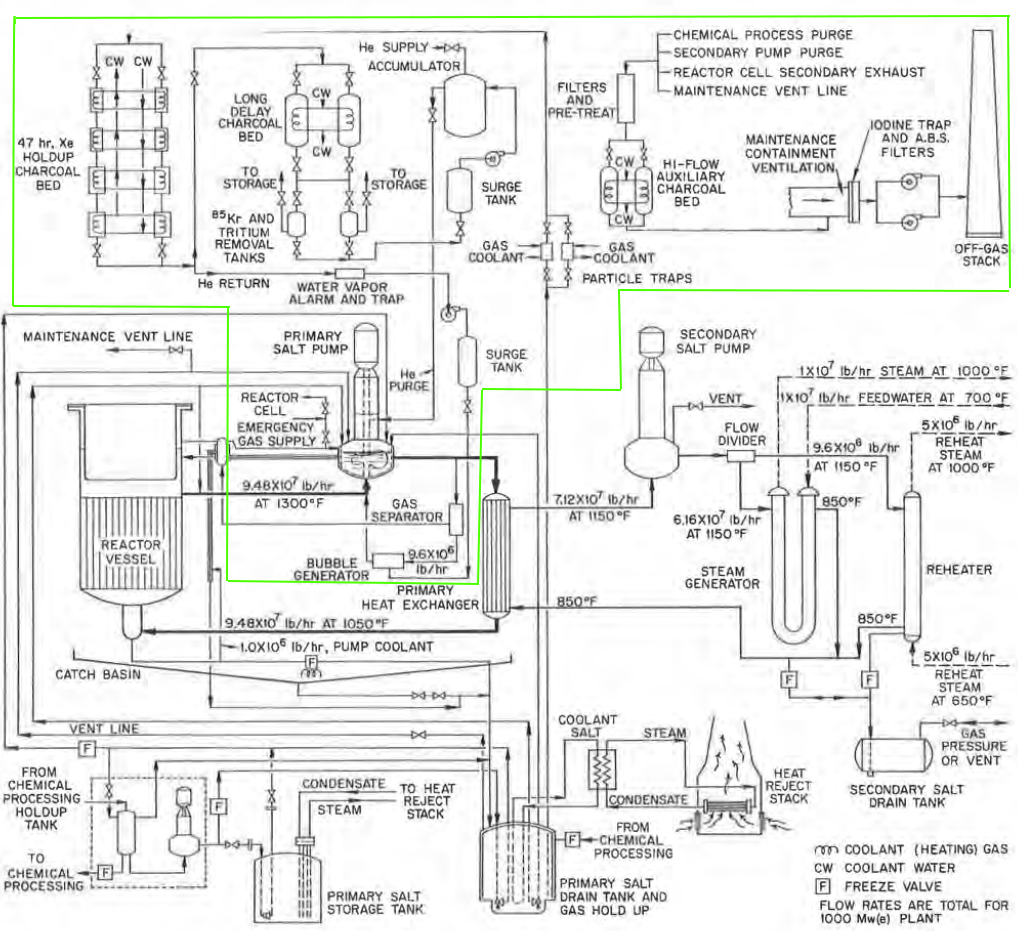
\includegraphics[width=1.05\textwidth]{gas_separation.png}
  \caption{Flow diagram for \gls{MSBR} plant. Green line indicates gas separation and off-gas system \cite{robertson_conceptual_1971}.}
  \vspace{-0.6em}
  \label{fig:gas_removal_system}
\end{figure}
\FloatBarrier
\section{Online reprocessing method}
Modeling liquid-fueled systems with existing neutron transport and depletion tools is challenging because most of these tools are designed for the solid-fueled reactors simulation. The fuel material flows and potential online separations or feeds of specific elements or nuclides are the main challenges of liquid-fueled systems. SaltProc accounts for online feeds and separations using SERPENT 2 neutron transport and burnup capabilities.

\subsection{Online separations and feeds}
The ability to perform online fuel salt reprocessing improves the potential neutronic performance of liquied-fueled reactors. Firstly, it is unnecessary for liquid-fueled reactors to operate with excess reactivity because fissile material is continuously being added into the core. Secondly, continuously removing fission products including strong absorbers (poisons) should significantly improve fuel utilization and decrease parasitic neutron absorption. Finally, neutronic parameters could be adjusted ``on-the-fly" without operational cycle interruption. Nevertheless, removal of each element from the liquid fuel salt presents a unique challenge in terms of storage and disposal of the separated materials.

To take into account online reprocessing two potential approaches can be implemented. One is a batch-wise approach where material is moved into or from the core at specific time intervals (batch). This approach assumes that material accumulation in the core during the time between separations or feeds does not affect on reactor physics. This method requires the simulation to stop, modify the fuel composition, and restart. This approach was implemented in a ChemTriton script \cite{powers_new_2013} which has been developed by T.J.Harrision, \gls{ORNL}, and actively using for online reprocessing simulation with SCALE/TRITON \cite{bowman_scale_2011} and Shift \cite{pandya_implementation_2016}. 

Another approach approximates more continuous reprocessing where material is separated from (or added into) the core at all times to exactly simulate true continuous online reprocessing. This method is more difficult because it requires adding a term to the Bateman equations. In SCALE/TRITON, ORIGEN \cite{gauld_isotopic_2011} solves a set of Bateman equations using one-group averaged fluxes and cross-sections obtained from a transport calculation. Bateman equations that describe the rate of change of the isotopes due to neutron induced reactions and decay
processes could be written in this form \cite{aufiero_extended_2013}:

\begin{align}
        \frac{dN_i}{dt} &= \bar{\Phi}\sum\limits_{j}N_{j}\sigma_{j \rightarrow 		i} - \bar{\Phi}\sum\limits_{j}N_{i}\sigma_{i \rightarrow j} + \sum					\limits_{j}	N_{j}\lambda_{j}b_{j \rightarrow i} - N_{i}\lambda_{i}
\label{eq:bateman}
	\intertext{where} 
	N_i &= \mbox{number density of isotope i} \\
	N_j &= \mbox{number density of isotope j} \\
	\bar{\Phi} &= \mbox {average in the space and energy neutron flux} \\
	\sigma_{j \rightarrow i} &= \mbox{microscopic one-group transmutation 			cross section} \\
	\lambda_i &= \mbox{decay constant of nuclide i} \\
	\lambda_j &= \mbox{decay constant of nuclide j} \\
	b_{j \to i} &= \mbox{branching fraction for neutron absorption}
\end{align}

The four terms on the right-hand side of the equation represent (1) the production rate of nuclide $i$ from irradiation, (2) the loss rate of nuclide $i$ due to irradiation, (3) the decay rate of nuclide $i$ into nuclide $j$, and (4) the loss rate of nuclide $i$ due to decay. Mentioned earlier deterministic codes SCALE/TRITON and Monte Carlo codes MCNP, Shift, KENO-VI do not support non-zero removal or feeds rates for depletion simulations.

Online fuel reprocessing can be explicitly introduced in the system of equations by adding effective decay and transmutation terms for the various nuclides. During fuel composition evolution calculations, the total mass fraction of thorium fluoride is kept constant at 12\%. For this purpose, $^{233}$Th isotope is replaced with the fresh $^{232}$Th feed material. This could be achieved with an additional gain term on the right-hand side of the Bateman equation:
\begin{align*}
\bar{\Phi}\sum\limits_{k=^{232}Th}N_{k}\sigma_{k,c}
\end{align*}
where $\sigma_{k,c}$ is the one-group capture cross section of thorium-232.

The removal of fission products and protactinium is achieved by adding an explicit decay term to the Bateman equations. For the generic fission product, l, loss term can be added:
\begin{align*}
- N_{l}\lambda_{l,reproc}
\end{align*}
where $\lambda_{l,reproc}$ is the effective removal time constant of the particular chemical species. This approach was recently implemented as a purpose-made extension within the continuous-energy Monte Carlo reactor physics and burn-up code SERPENT \cite{aufiero_extended_2013} but it is not properly tested and or available for ordinary users at present.

I have developed the SaltProc Python package \cite{andrei_rykhlevskii_arfc/saltproc:_2018}, implementing batch-wise approach coupled with the SERPENT 2 burnup routine. A high-fidelity full-core \gls{MSBR} model serves as a basis for the online reprocessing simulation described in this thesis. Assessment against the SERPENT 2 continuous online reprocessing procedure based on the basis is not treated here.

\subsection{Fuel material flows}
The $^{232}$Th in the fuel absorbs thermal neutrons and produces $^{233}$Pa which then decays into the fissile $^{233}$U. Furthermore, the \gls{MSBR} design requires online reprocessing to remove all poisons (e.g. $^{135}$Xe), noble metals, and gases (e.g. $^{75}$Se, $^{85}$Kr) every 20 seconds. Protactinium presents a challenge, since it has a large absorption cross section in the thermal energy spectrum. Accordingly, $^{233}$Pa is continuously removed from the fuel salt into a protactinium decay tank to allow $^{233}$Pa to decay to $^{233}$U without poisoning the reactor. The reactor reprocessing system is designed to separate $^{233}$Pa from the molten-salt fuel over 3 days, hold it while $^{233}$Pa decays into $^{233}$U, and return it back to the primary loop. This feature allows the reactor to avoid neutron losses to protactinium, keeps fission products to a very low level, and increases the efficiency of $^{233}$U breeding. Table~\ref{tab:reprocessing_list} summarizes full list of nuclides and the cycle times used for modeling salt treatment and separations \cite{robertson_conceptual_1971}. 

%%%%%%%%%%%%%%%%%%%%%%%%%%%%%%%%%%%%%%%%
\begin{table}[ht!]
        \centering
        \caption{The effective cycle times for protactinium and fission product removal \cite{robertson_conceptual_1971}.}
        \begin{tabular}{|m{0.25\textwidth} | m{0.45\textwidth}|m{0.20\textwidth}|}
        \hline 
        %\begin{tabularx}{\linewidth}{l X} \toprule 
        Processing group & \qquad\qquad\qquad Nuclides & Cycle time (at full power) \\ [5pt] \hline 
        Rare earths & Y, La, Ce, Pr, Nd, Pm, Sm, Gd & 50 days \\ [5pt] \hline 
        \qquad & Eu & 500 days \\ [5pt] \hline
        Noble metals & Se, Nb, Mo, Tc, Ru, Rh, Pd, Ag, Sb, Te & 20 sec \\ [5pt] \hline
        Seminoble metals & Zr, Cd, In, Sn & 200 days \\ [5pt] \hline
        Gases & Kr, Xe & 20 sec \\ [5pt] \hline
        Volatile fluorides & Br, I & 60 days \\ [5pt] \hline
        Discard & Rb, Sr, Cs, Ba & 3435 days \\ [5pt] \hline
        Salt discard & Th, Li, Be, F & 3435 days \\ [5pt] \hline
        Protactinium & $^{233}$Pa & 3 days \\ [5pt] \hline
        Higher nuclides & $^{237}$Np, $^{242}$Pu & 16 years \\ [5pt] \hline
        \end{tabular}
        \label{tab:reprocessing_list}
          \vspace{-0.9em}
\end{table}
Since removal rates vary among nuclides in this reactor concept, the built-in SERPENT 2 reprocessing subroutine is unable to capture the desired reprocessing strategy. The removal rates also dictate the necessary resolution of depletion calculations. If the depletion time intervals are very short an enormous number of depletion steps are required to obtain the equilibrium composition. On the other hand, if the depletion  calculation time interval is too long, serious impacts of short lived fission products are not captured in a manner that is faithful to the \gls{MSBR} conceptual design. To compromise, the time interval for depletion calculations in this model was selected as 3 days to correlate with the removal interval of $^{233}$Pa and thorium-232 was continuously added to maintain the initial mass fraction of $^{232}$Th.

\subsection{Simplifying assumptions}
The main goal of the present study is to identify the effects adjusting the fuel salt composition, and find equilibrium performance of a thorium \gls{MSBR} fuel cycle. To highlight these effects and simplify the analyses, several assumptions have been made.

First of all, thorium loading during operation was held constant and equal to initial thorium loading (i.e. $m_{Th}(t)=m_{Th}(0)$) with a variable feed rate (in kg/day) of fresh thorium. Because thorium is a fertile material with relatively high absorption cross section, this has important impacts on reactor physics, including negatively impacting reactivity and distorting the fuel-to-moderator ratio which makes neutron energy spectrum harder. While a reduction in the thorium loading reduces the amount of initial fissile material required to achieve criticality, the breeding rate of $^{233}$U should be sufficient to maintain the core critical during operation.

The solubility of heavy metals is a known problem for \glspl{MSR} but it is fundamentally dependent on the type of carrier salt. For this work, solubility limits for uranium were neglected because the molar fraction of UF$_4$ was negligible for the accuracy desired in this work. In addition, this work assumed that addition or removal of soluble material (e.g. UF$_4$) has a small influence on the fuel salt volume, this volume change is not treated here.

Figure~\ref{fig:th_cycle} from Chapter 2 demonstrates that transformation from $^{232}$Th to $^{233}$U takes about 30 days because $^{233}$Pa $\beta$-decay has half-life 27.4 days. Figure~\ref{fig:pa_isolation} shows how protactinium is separated from the fuel salt reprocessing flow. Therefore, if protactinium decay tank is empty at the moment of reactor startup, then the expected fissile material stream would appear only after a few weeks of reactor operation at full power. To avoid time-dependent feed rate for $^{233}$UF$_4$ it is assumed that the protactinium decay tank initially contain some amount of $^{233}$UF$_4$, and the rate of fissile material flow from the tank to the core is set equal to the $^{233}$Pa removal rate. Moreover, simulated cycle time at full power in this study was limited by 20 years ($\approx$ 7300 days). Finally, 100\% reprocessing separation efficiency was assumed.

\begin{figure}[hbp!] % replace 't' with 'b' to 
  \centering
  \vspace{-0.3em}
  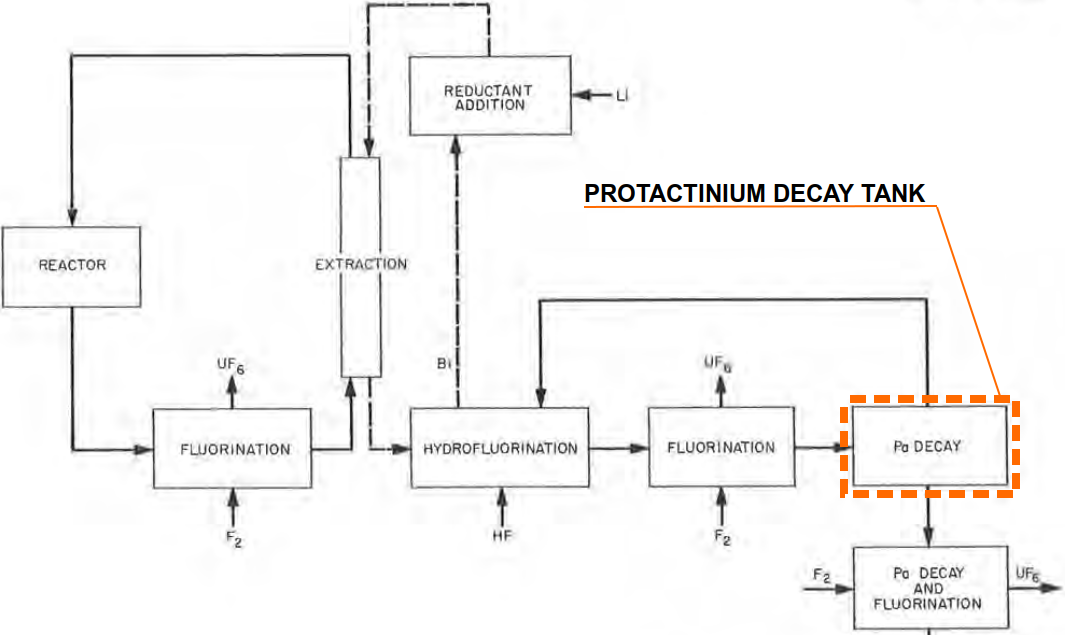
\includegraphics[width=\textwidth]{pa_isolation.png}
  \caption{Protactinium isolation with uranium removal by fluorination \cite{robertson_conceptual_1971}.}
  \vspace{-0.6em}
  \label{fig:pa_isolation}
\end{figure}
\FloatBarrier

The thermal fission of a $^{233}$U in fluoride salts oxidizes the salt. This happens because the uranium nucleus balances the charge of four fluorine ions in the salt (e.g. $^{233}$UF$_4$), but fission products tend to not bind to all the four fluorines released after the uranium fissions. Figure~\ref{fig:excess_fluorine} demonstates an example of an oxidative fission reaction. This excess of fluorine must be compensated, otherwise chemical reactions harmful to reactor components would occur \cite{ridley_method_2017}. In this study, fission-driven salt oxidation is ignored.

\begin{figure}[htp!] % replace 't' with 'b' to 
  \centering
  \vspace{-0.3em}
  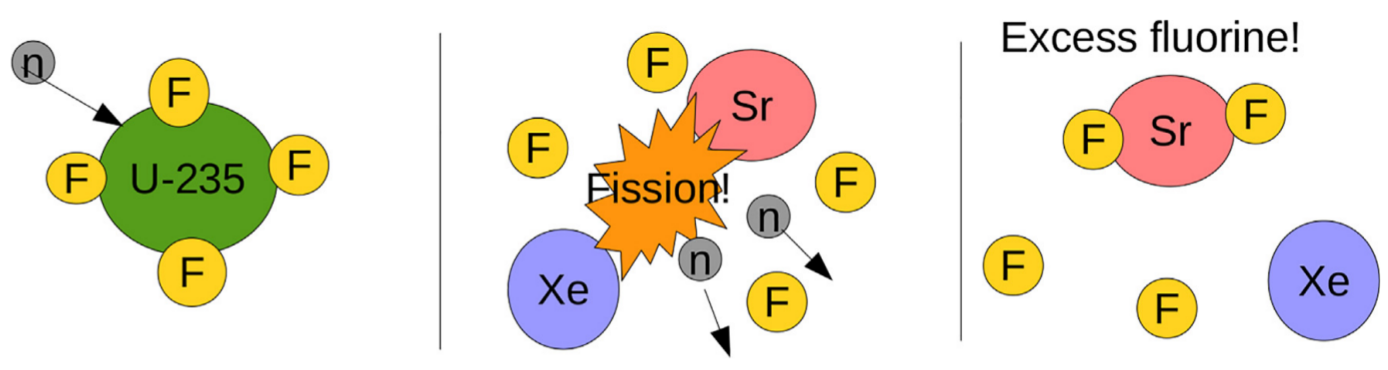
\includegraphics[width=0.8\textwidth]{excess_fluorine.png}
  \caption{Process of production an excess of fluorine due to fission of a $^{233}$U in fluoride salts \cite{ridley_method_2017}.}
  \vspace{-0.6em}
  \label{fig:excess_fluorine}
\end{figure}
\FloatBarrier

Finally, for this study, equilibrium is defined as when $k_{eff}$ and the $^{233}$U concentration in the fuel salt vary less than one percent over several months. 

\section{Python code description}
The objectives for the SaltProc tool were to expand SERPENT 2 burn-up capabilities for modeling liquid-fueled \gls{MSR} and provide an open-source tool for the simulation of reactors where material is removed or added at any time during fuel irradiation. The Python 2.7 packages uses HDF5 \cite{the_hdf_group_hierarchical_nodate} to store data and the Nuclear Engineering Toolkit - PyNE \cite{scopatz_pyne:_2012} for SERPENT output file parsing. As was discussed earlier, SaltProc maintains the iterative semi-continuous approach to simulate continuous feeds and removals.

The tool structure and capabilities are similar to ChemTriton tool for SCALE developed in \gls{ORNL} \cite{powers_new_2013}. SaltProc coupled with Monte Carlo SERPENT 2 software which allows to simulate online reprocessing for irregular full-core geometry with high level of fidelity.  The primary function of SaltProc is to manage material mixtures while SERPENT 2 performs most of the computationally heavy work namely neutron transport and burnup calculations. Each material stream represents a fluid in the core design and has specific parameters (e.g. isotopic composition, reprocessing interval, mass rate, removal efficacy, etc). In addition, SaltProc provides a set of available functions for each stream: read and write isotopic data in/from database, separate out specific isotopes from stream with defined efficiency, feed in specific isotopes to stream, and maintain constant number density of specific nuclide in the core. These attributes and functions are crucial to simulate the operation of a complex, multi-zone, multi-fluid \gls{MSR} and are universal enough for myriad reactor systems.

Figure~\ref{fig:saltproc_flow} demonstrates the  online reprocessing simulation algorithm coupling SaltProc and SERPENT 2. To perform depletion step, SaltProc reads a external SERPENT 2 template file which must be defined by user. This file contain input cards with all required for burnup calculations data such as geometry, moderator and construction materials isotopic composition, neutron population, criticality cycles, total heating power, boundary conditions. After depletion calculation completes, SaltProc reads the burned fuel composition file into memory and store it into HDF5 database. SaltProc only knows the number density and isotopic composition of a given fuel stream which provides the tool with the flexibility to model any geometry: an infinite medium, a unit cell, a multi-zone simplified assembly, or a full-core. While in some applications the simple sigle-cell is sifficient to get an accurate results within the fuel for depletion calculations with reduced simulation time, this flexibility provides high-fidelity full-core geometry capabilities for comparisons to more scrupulous models.

SaltProc could manage as many fuel streams as desired. It also may work with multiple depletion materials. At the end of a each depletion step, SaltProc reads the separate depleted compositions and tracks each material stream individually. Following this, chemical reprocessing functions applying to fuel stream vectors. These vectors then combining in matrix, storing in database and printing into SERPENT composition file for the next step calculations.

Liquid-fueled \gls{MSBR} design focuses on the state of the core at an equilibrium condition, after fission products have built up in the fuel salt during years if operation. Changes in isotopic composition of the fuel salt continues encounter small changes even after decades of operation, but the dominant nuclides that have significant impact to the neutronics behavior tend to reach an equilibrium concentration (e.g., vary less than 1\% over several years). In contrast, from the startup of an \gls{MSBR} until equilibrium condition, the fuel salt composition undergo significant changes (e.g., fission producs, minor actinides, and fissile materials number density). During this period, the material feeds and removals should be optimized for the fastest \gls{MSBR} transition to an equilibrium state, where the material streams are more constant in time. A faster transition simplifies the reactor operation because in an equilibrium state the fissile and fertile feed rates, safety parameters, and fission product removal rates are more constant in time.

\begin{figure}[htp!] % replace 't' with 'b' to 
  \centering
  \vspace{-0.3em}
  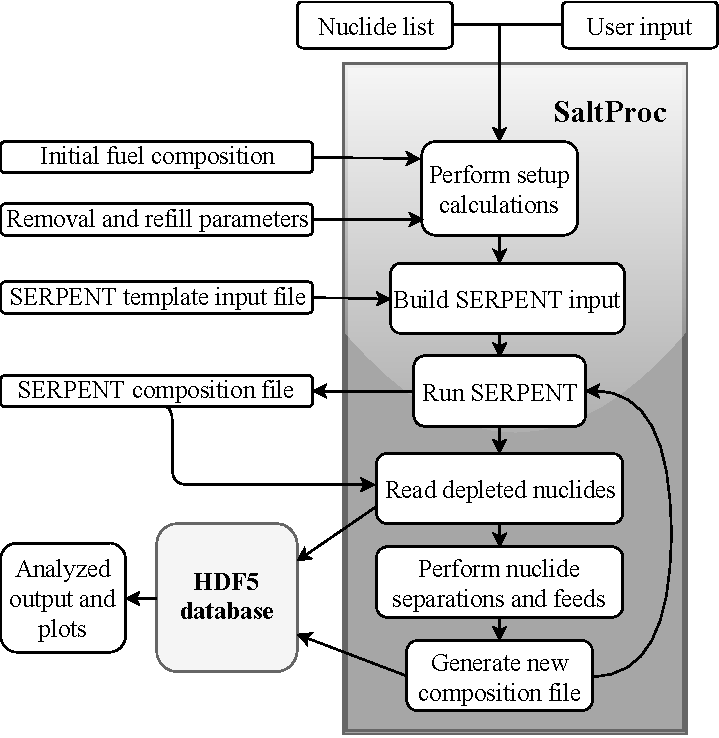
\includegraphics[width=\textwidth]{saltproc_flowchart.pdf}
  \caption{Flow chart for the Saltproc python-based tools.}
  \vspace{-0.6em}
  \label{fig:saltproc_flow}
\end{figure}
\FloatBarrier

In addition, SaltProc is able to define time-dependent material feed and removal rates to investigate the effect of different nuclide separations and/or feeds. The time dependence of the streams could be define as piecewise functions and could be dependent on certain conditions being met. For instance, the tool could increase fissile material feeding rate if effective multiplication factor, $k_{eff}$, below a specific limit. Moreover, it could be useful to keep fissile material number density in the core approximately constant to accumulated excess of $^{233}$U into protactinium decay tank. These capabilities allow SaltProc to investigate the effect of lower concentrations of fissile and fertile startup loads. In sum, the development approach of SaltProc focused on producing a generic and flexible tool to give SERPENT 2 Monte Carlo code the ability to conduct advanced fuel cycle analysis as well as simulate a myriad of online refueled systems.

\chapter[Results]{Results}

This chapter presents calculation results based on the methodology described in Chapters 3 and 4. The effective multiplication factor, number density of major isotopes, and $^{232}$Th refill rate are calculated using a full-core SERPENT 2 model with 3-day depletion steps over a 20-year operation. Moreover, neutron flux, neutron energy spectrum, temperature reactivity coefficients, control rod worth, power density, and $^{233}$U breeding density distribution are presented for both initial and equilibrium fuel salt composition. The neutron flux and energy spectrum are calculated for the full-core model, normalized by neutron lethargy and reported for each zone. The temperature coefficients of reactivity for both the fuel salt and graphite components are estimated at the initial state by comparing effective multiplication factors at temperatures uniformly distributed from 900K and 1000K. The rod worth is calculated at several different insertion levels of control and safety rods. Finally, six factor analysis was performed to show evolution of these parameters during reactor operation.

The neutron population per cycle and the number of active/inactive cycles were chosen to obtain balance between reasonable uncertainty for a transport problem ($\leq$ 40 pcm for effective multiplication factor) and computational time. The \gls{MSBR} depletion and safety parameter computations were performed on 64 Blue Waters XK7 nodes (two AMD 6276 Interlagos CPU per node, 16 floating-point Bulldozer core units per node or 32 ``integer" cores per node, nominal clock speed is 2.45 GHz). The total computational time for achieving equilibrium composition was approximately 9,000 node hours (144,000 core hours.)

\section{Effective multiplication factor}
Figure~\ref{fig:keff} demonstrates the effective multiplication factors obtained using SaltProc and SERPENT 2. The effective multiplication factors are calculated after removing fission products listed in Table~\ref{tab:reprocessing_list} and adding the fertile material at the end of ``cycle time"\footnote{The \gls{MSBR} program defined a ``cycle time" as the amount of time required to remove 100\% of a target nuclide from a fuel salt.} which was fixed at 3 days for this work. The effective multiplication factor fluctuates significantly as a result of the batch-wise nature of this online reprocessing strategy. 
\begin{figure}[hbp!] % replace 't' with 'b' to 
  \centering
  \vspace{-0.3em}
  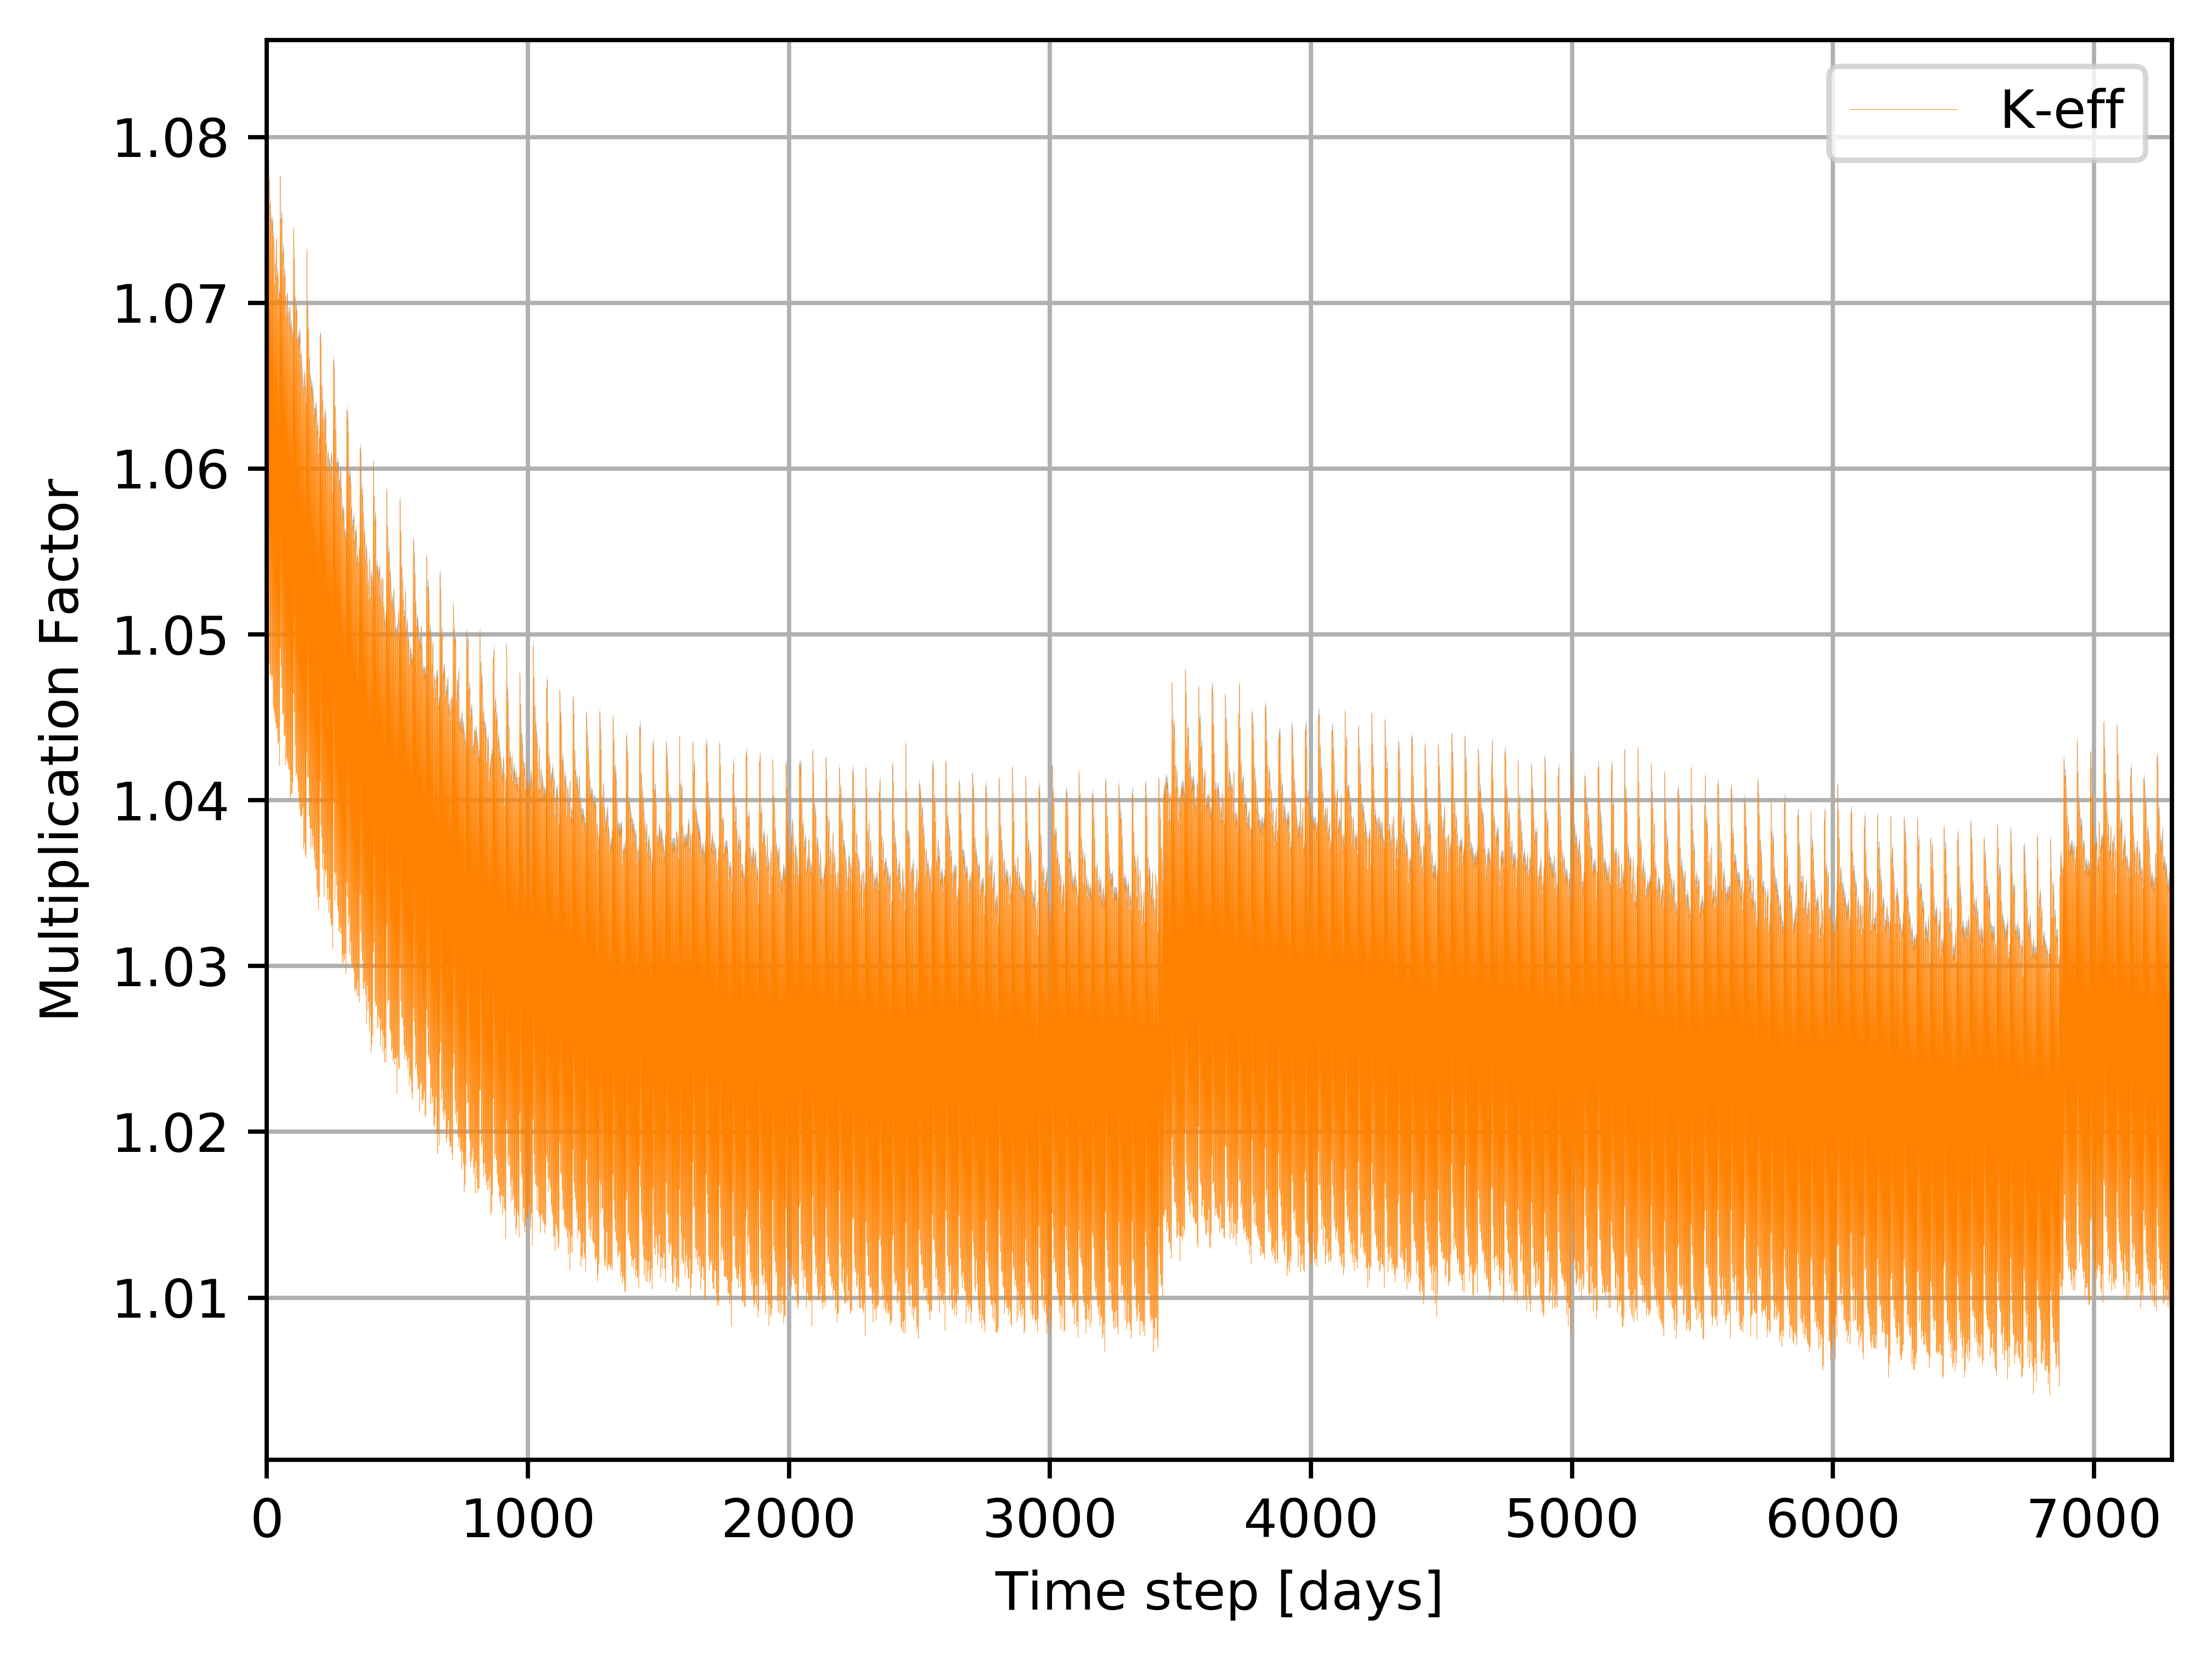
\includegraphics[width=\textwidth]{keff.png}
  \caption{Effective multiplication factor dynamics for full-core \gls{MSBR} model for a 20-year reactor operation. The confidence interval $\pm\sigma$ is shaded.}
  \vspace{-0.6em}
  \label{fig:keff}
\end{figure}
\FloatBarrier

First, SERPENT calculates the effective multiplication factor for the beginning of cycle time (fresh fuel composition for the first step). Next, it computes the new fuel salt composition for the end of a 3-day depletion step. The corresponding effective multiplication factor is much smaller than the previous one. Finally, SERPENT calculates $k_{eff}$ for the depleted composition after applying feeds and removals, and this increases accordingly since major reactor poisons (e.g. Xe, Kr) are removed, while fresh fissile material ($^{233}$U) from the protactinium decay tank is added. 

Additionaly, the presence of rubidium, strontium, cesium, and barium in the core are disadvantageous to reactor physics. In fact, removal of these elements every 3435 days causes the multiplication factor to jump by approximately 450 pcm, and limits using the batch approach for online reprocessing simulation. Overall, the effective multiplication factor gradually decreases from 1.075 to $k_{eff} \approx 1.02$ at equilibrium after approximately 6 years of irradiation. 

The analysis of the fuel salt composition evolution provides more comprehensive information about the equilibrium state. Figure~\ref{fig:adens_eq} shows major nuclides which have a strong influence on the reactor core physics normalized separately for each isotope by average atomic density, at the beginning of each depletion time step. Concentration of $^{233}$U, $^{232}$Th, $^{233}$Pa, and $^{232}$Pa in fuel salt change insignificantly after approximately 2500 days of operation. Particularly, $^{233}$U number density fluctuates less than 0.8\% in the time interval from 16 to 20 years of operation, hence,a quasi-equlibrium state was achieved after 16 years of reactor operation.

In contrast, a wide variety of nuclides, including fissile isotopes (e.g. $^{235}$U) and non-fissile strong absorbers (e.g. $^{234}$U), keep accumulating in the core. Figures~\ref{fig:fissile_short}, \ref{fig:fissile_long} demonstrate production of short-life and long-life fissile isotopes in the core, respectively. In the end of considered operational time the core contains significant $^{235}$U ($\approx 9\times10^{-6}$ atom/b-cm), $^{238}$Pu ($\approx 10^{-6}$ atom/b-cm), $^{237}$Np ($\approx10^{-6}$ atom/b-cm), $^{232}$U ($\approx$10$^{-7}$ atom/b-cm), $^{239}$Pu ($\approx10^{-7}$ atom/b-cm), and $^{241}$Pu ($\approx 5\times10^{-8}$ atom/b-cm). Meanwhile, the equilibrium number density of the target fissile isotope $^{233}$U was approximately 7.97$\times10^{-5}$ atom/b-cm. Thus, production of new fissile materials in the core as well as $^{233}$U breeding make it possible to compensate for negative effects of strong absorber accumulation and keep the reactor critical.

\begin{figure}[htp!] % replace 't' with 'b' to 
  \centering
  \vspace{-0.3em}
  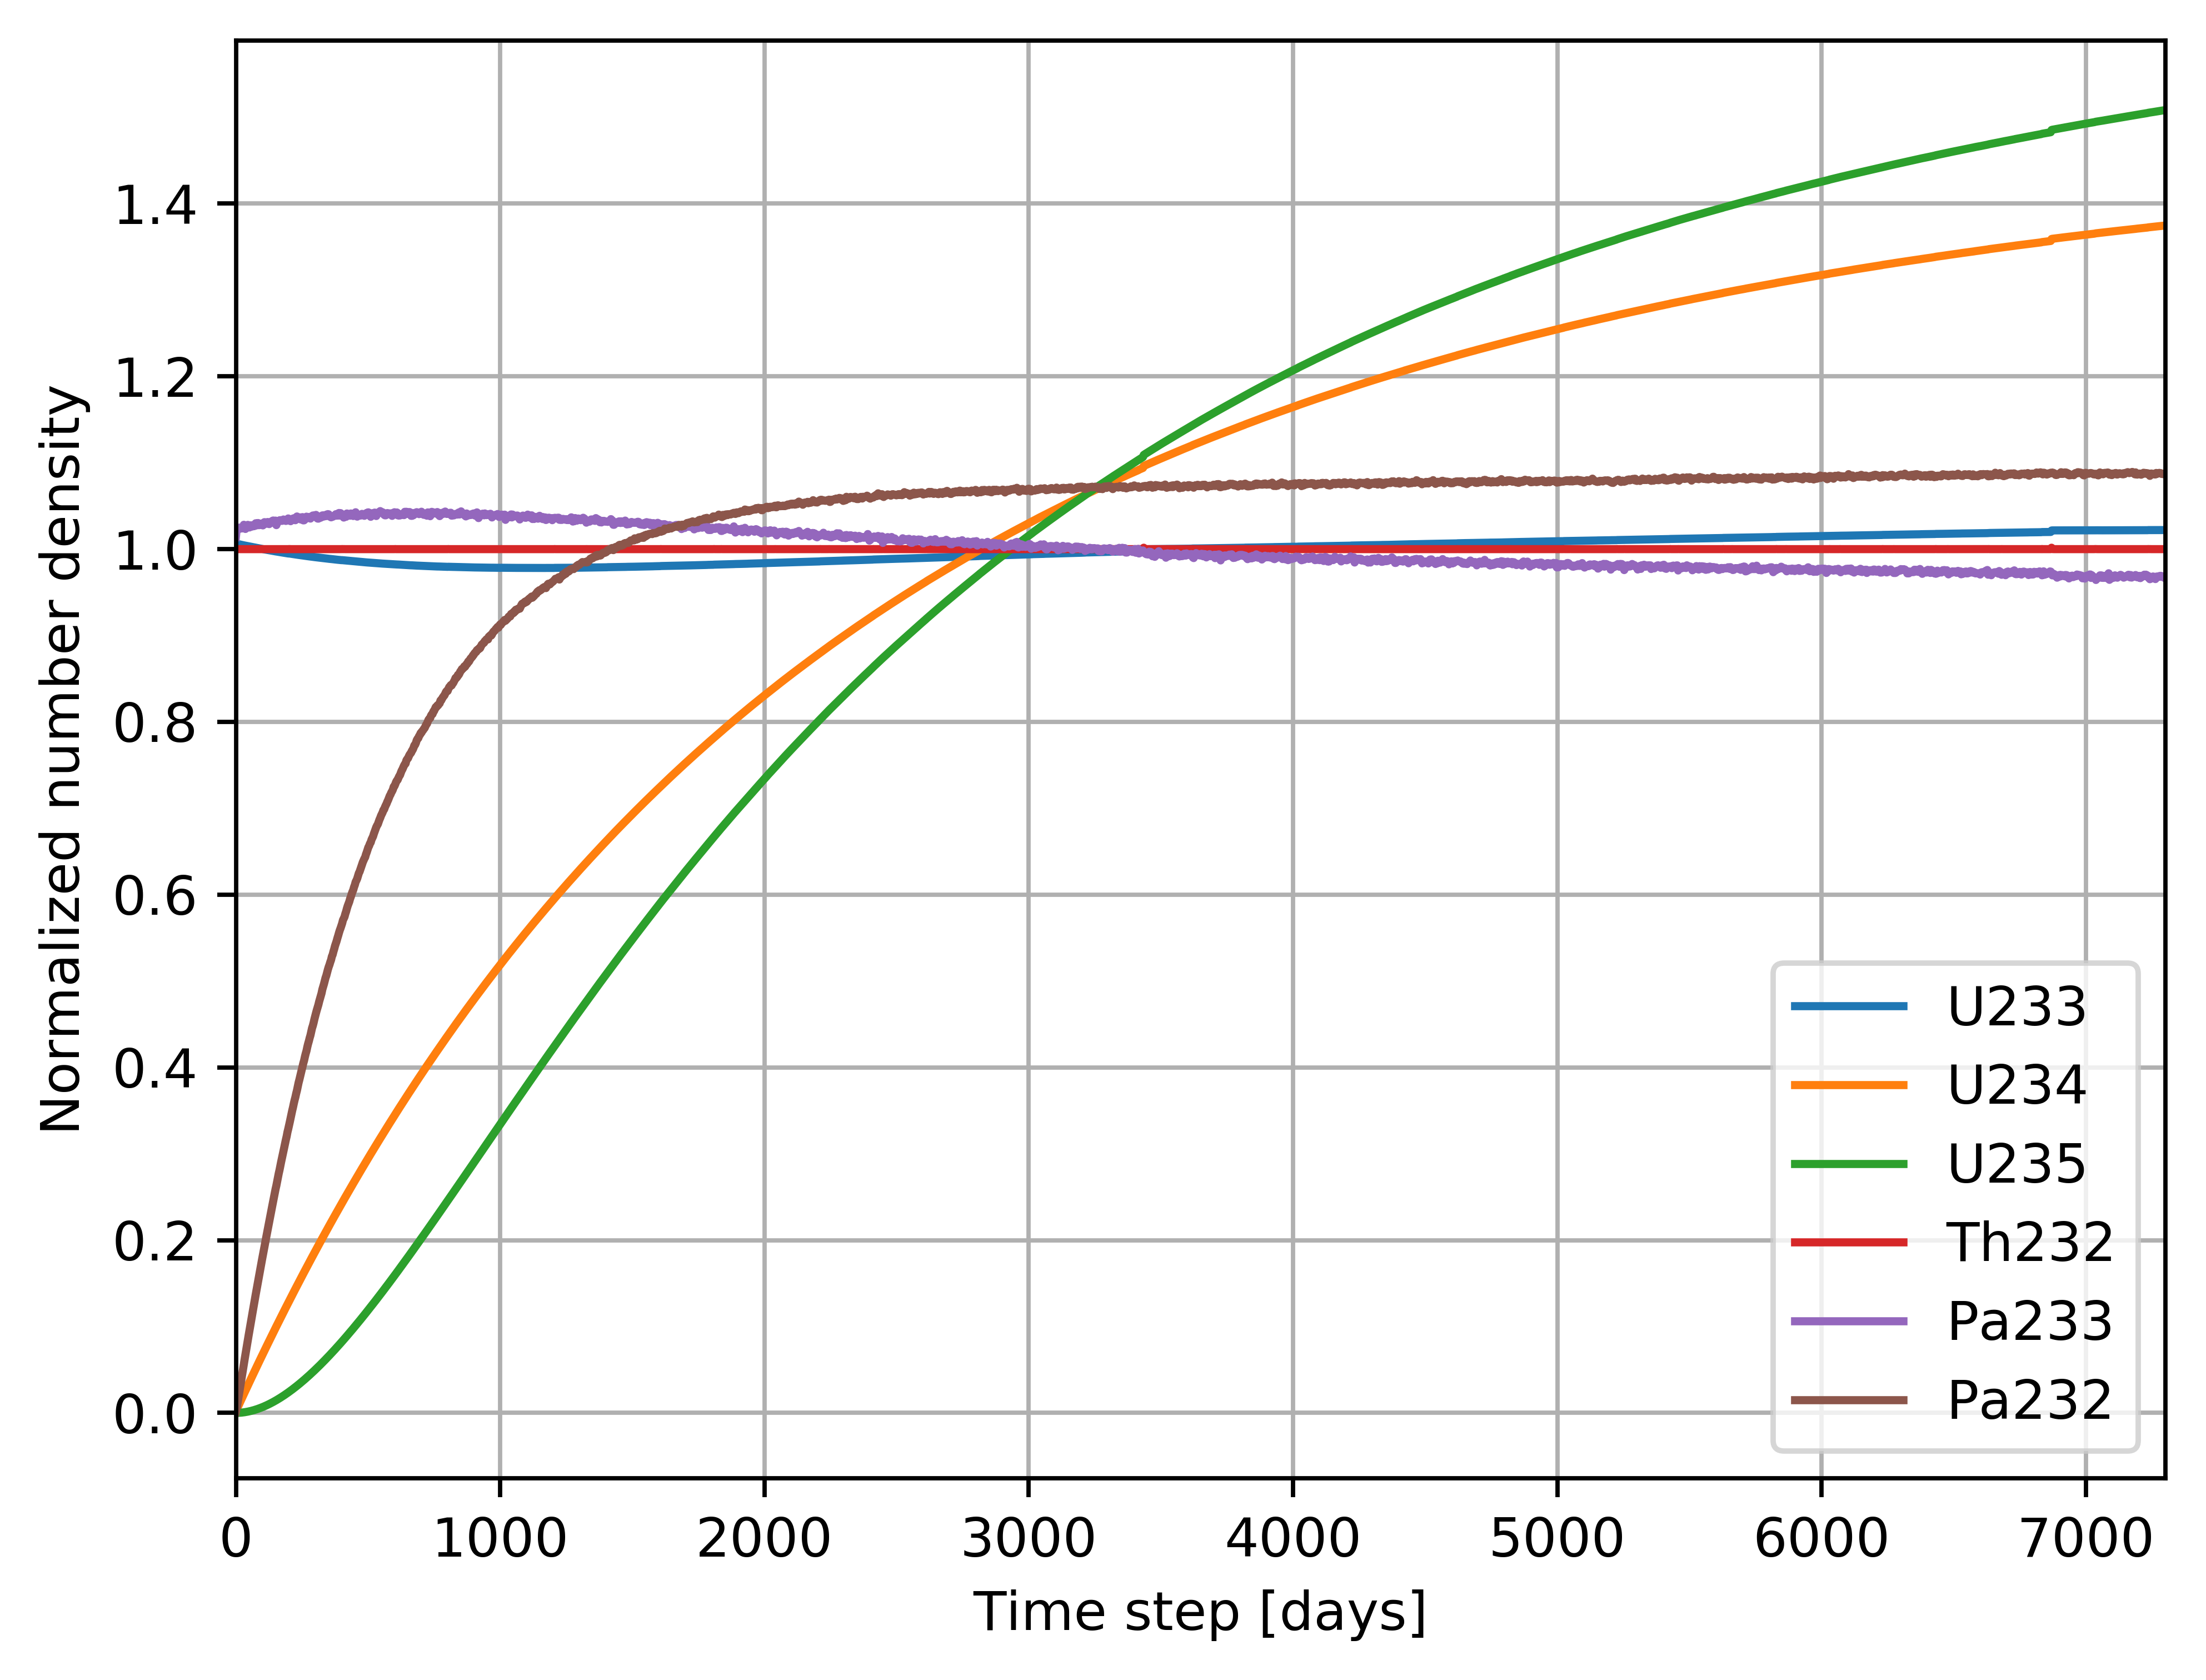
\includegraphics[width=\textwidth]{major_isotopes_adens.png}
  \caption{Normalized number density of major nuclides during the reactor operation.}
  \vspace{-0.6em}
  \label{fig:adens_eq}
\end{figure}
\FloatBarrier

\begin{figure}[htp!] % replace 't' with 'b' to 
  \centering
  \vspace{-1.3em}
  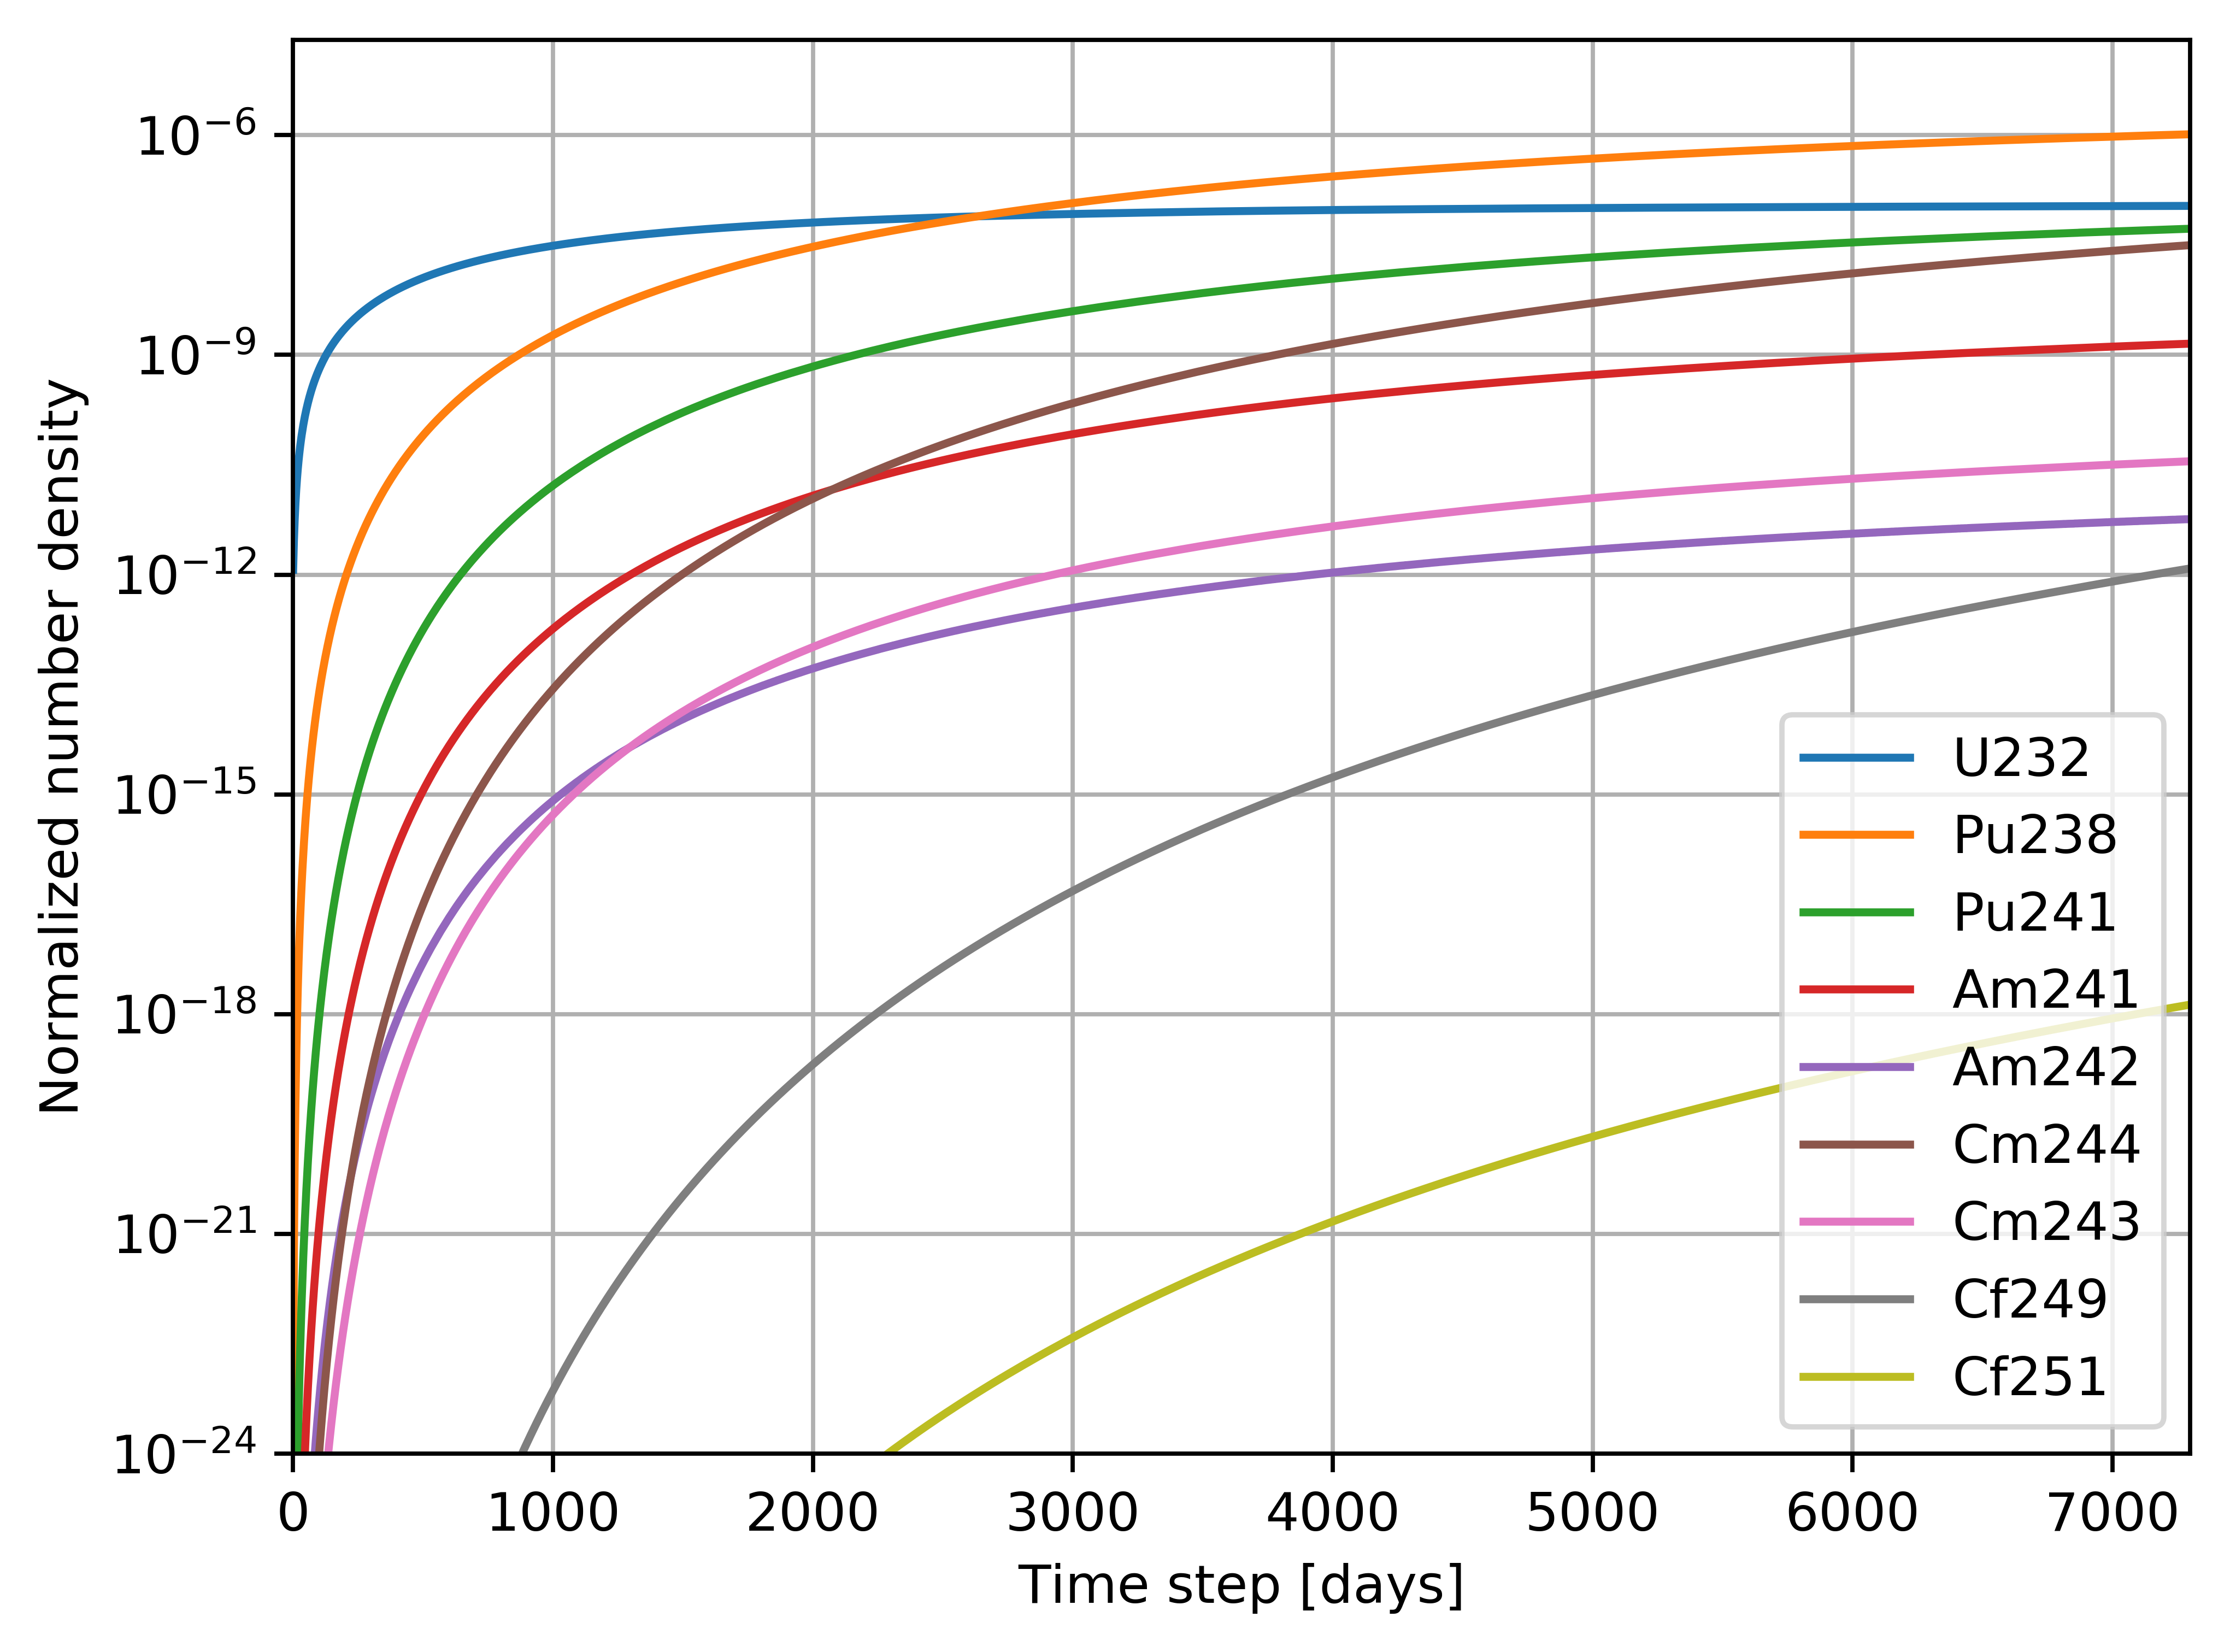
\includegraphics[width=\textwidth]{fissile_short.png}
   \vspace{-1.5em}
  \caption{Absolute number density of short-lived fissile nuclides ($\tau_{1/2}<900y$) during the reactor operation.}
  \vspace{-1.6em}
  \label{fig:fissile_short}
\end{figure}
\begin{figure}[hbp!] % replace 't' with 'b' to 
  \centering
  \vspace{-0.3em}
  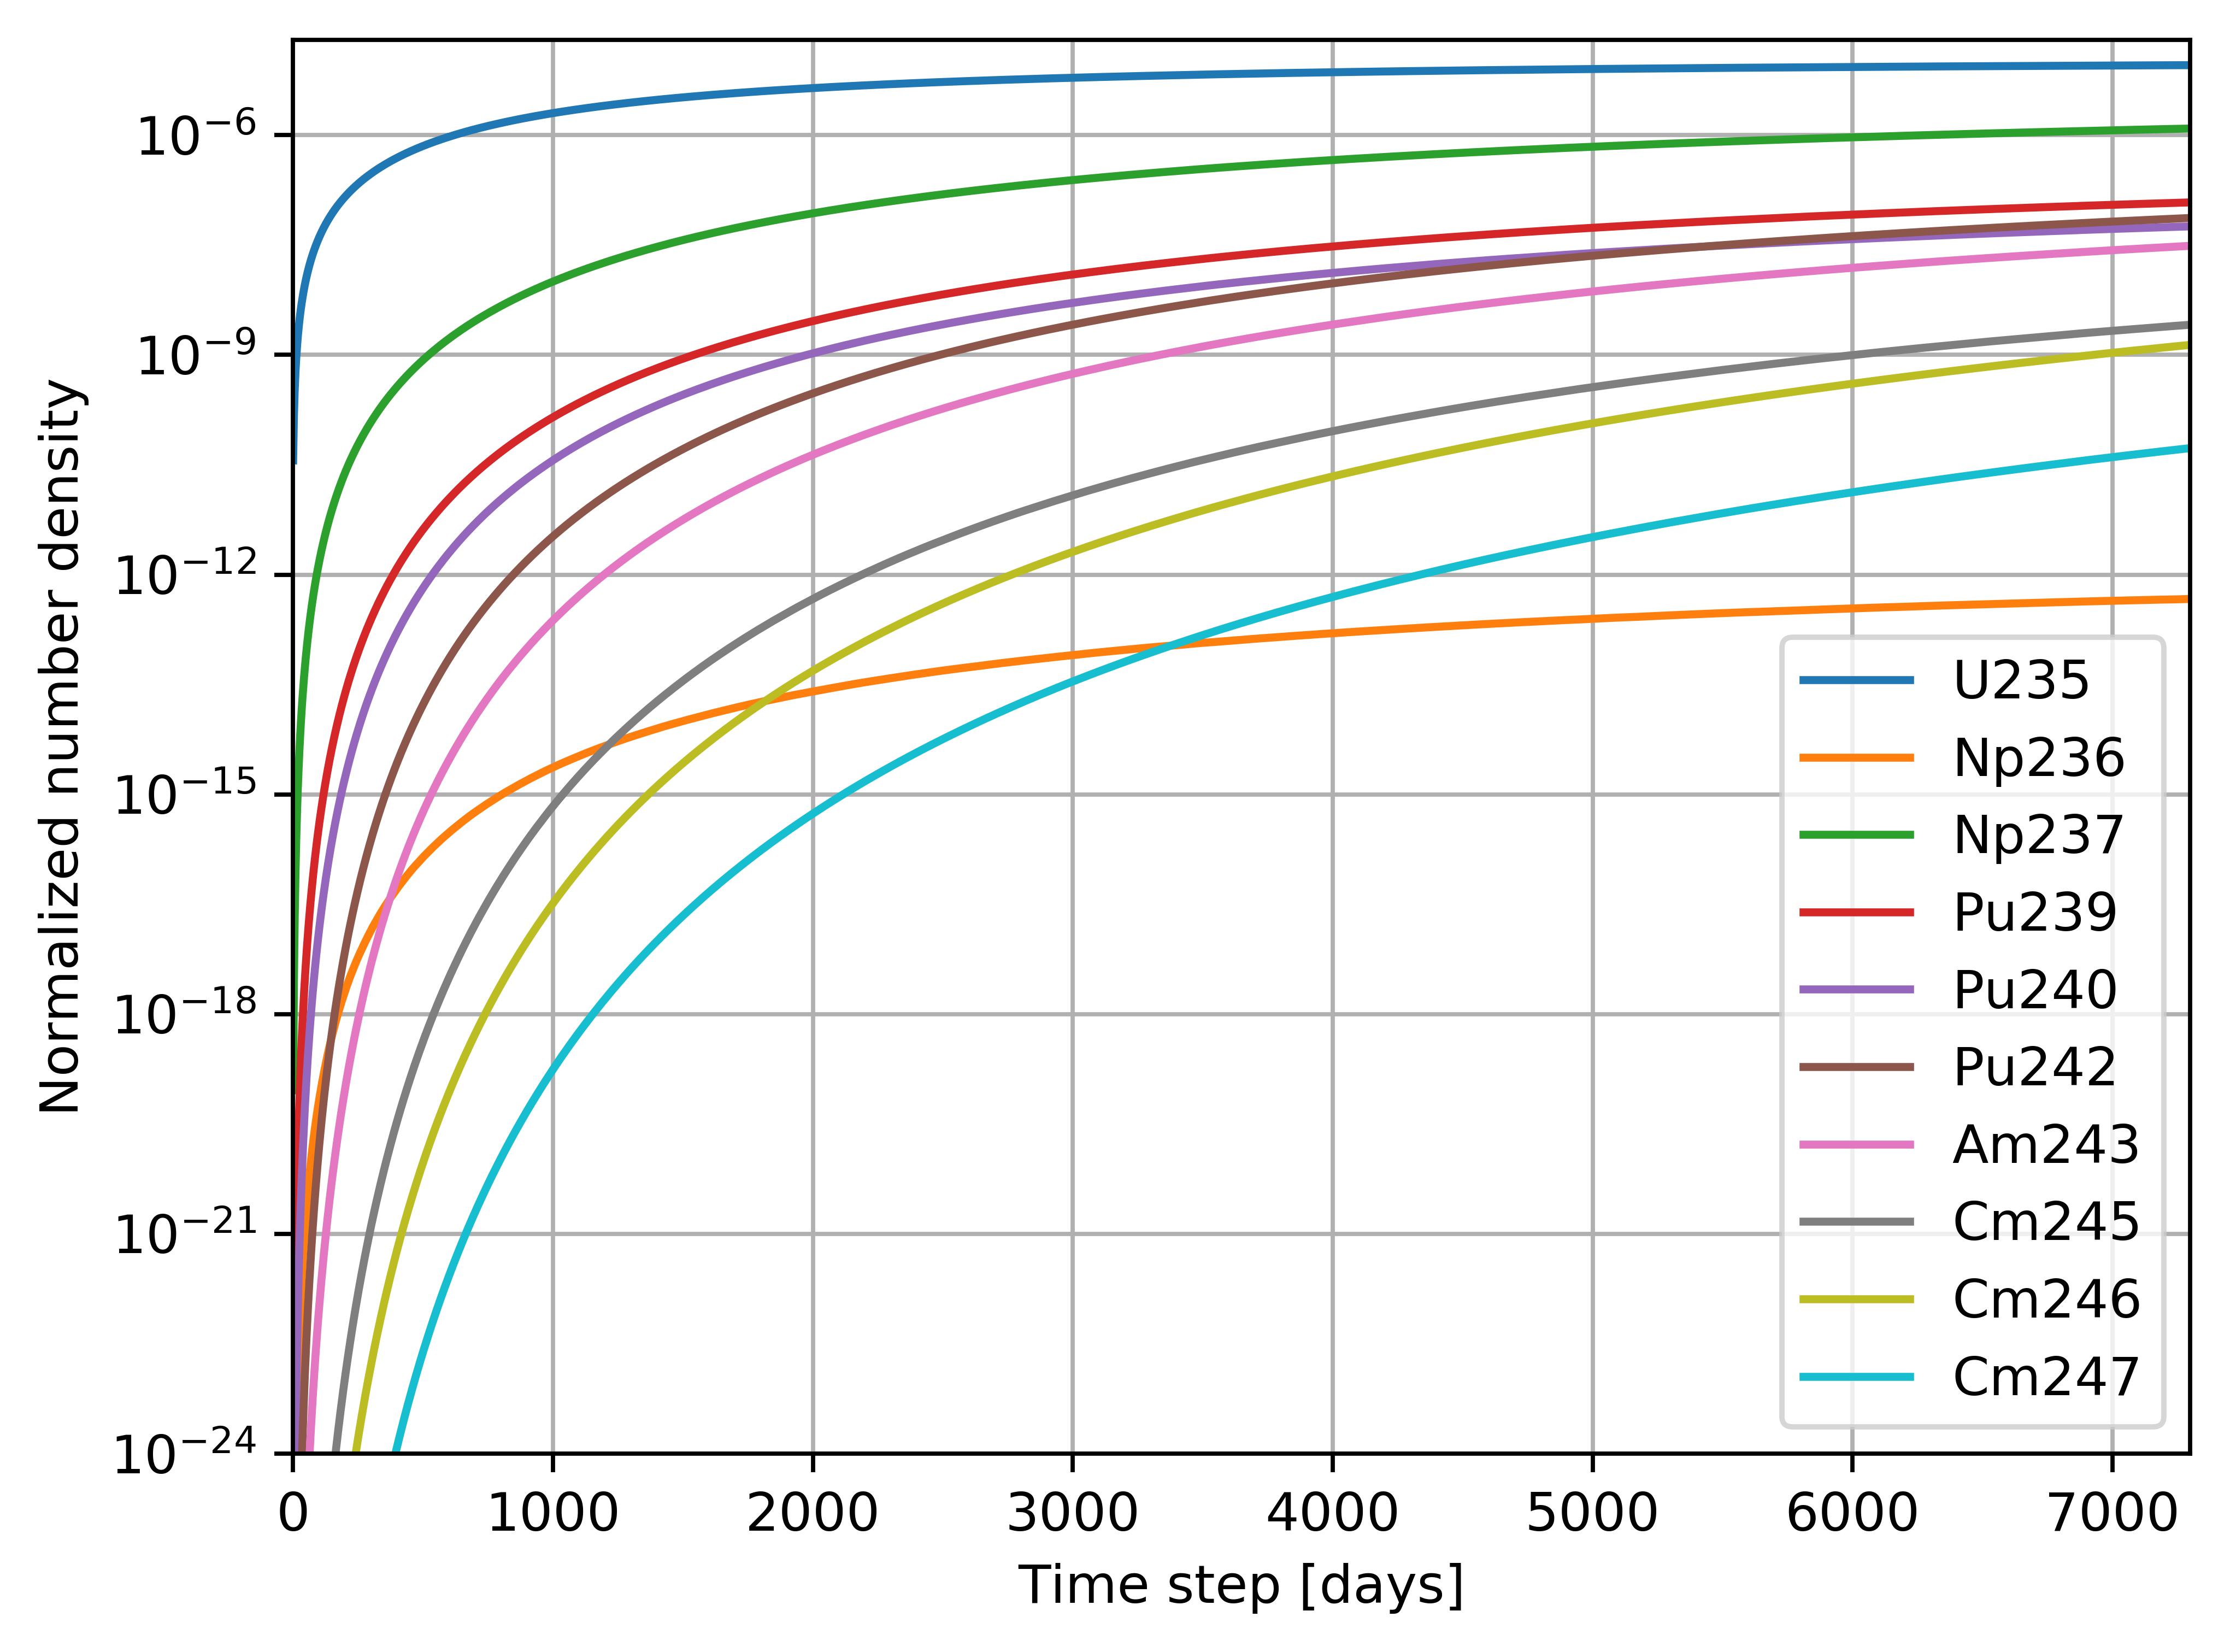
\includegraphics[width=\textwidth]{fissile_long.png}
   \vspace{-1.5em}
  \caption{Absolute number density of long-lived fissile nuclides ($\tau_{1/2}>900y$) during the reactor operation.}
  \vspace{-2.6em}
  \label{fig:fissile_long}
\end{figure}
\FloatBarrier

\section{Neutron spectrum}
Figure~\ref{fig:spectrum} shows the normalized neutron flux spectrum for the full-core \gls{MSBR} model in the energy range from $10^{-8}$ to $10$ MeV. The neutron energy spectrum at equilibrium is harder than at startup due to $^{238}$Pu, $^{239}$Pu, $^{240}$Pu, $^{241}$Pu, and $^{242}$Pu accumulation in the core during reactor operation. 

\begin{figure}[htp!] % replace 't' with 'b' to force it to 
  \centering
    \vspace{-0.3em}
  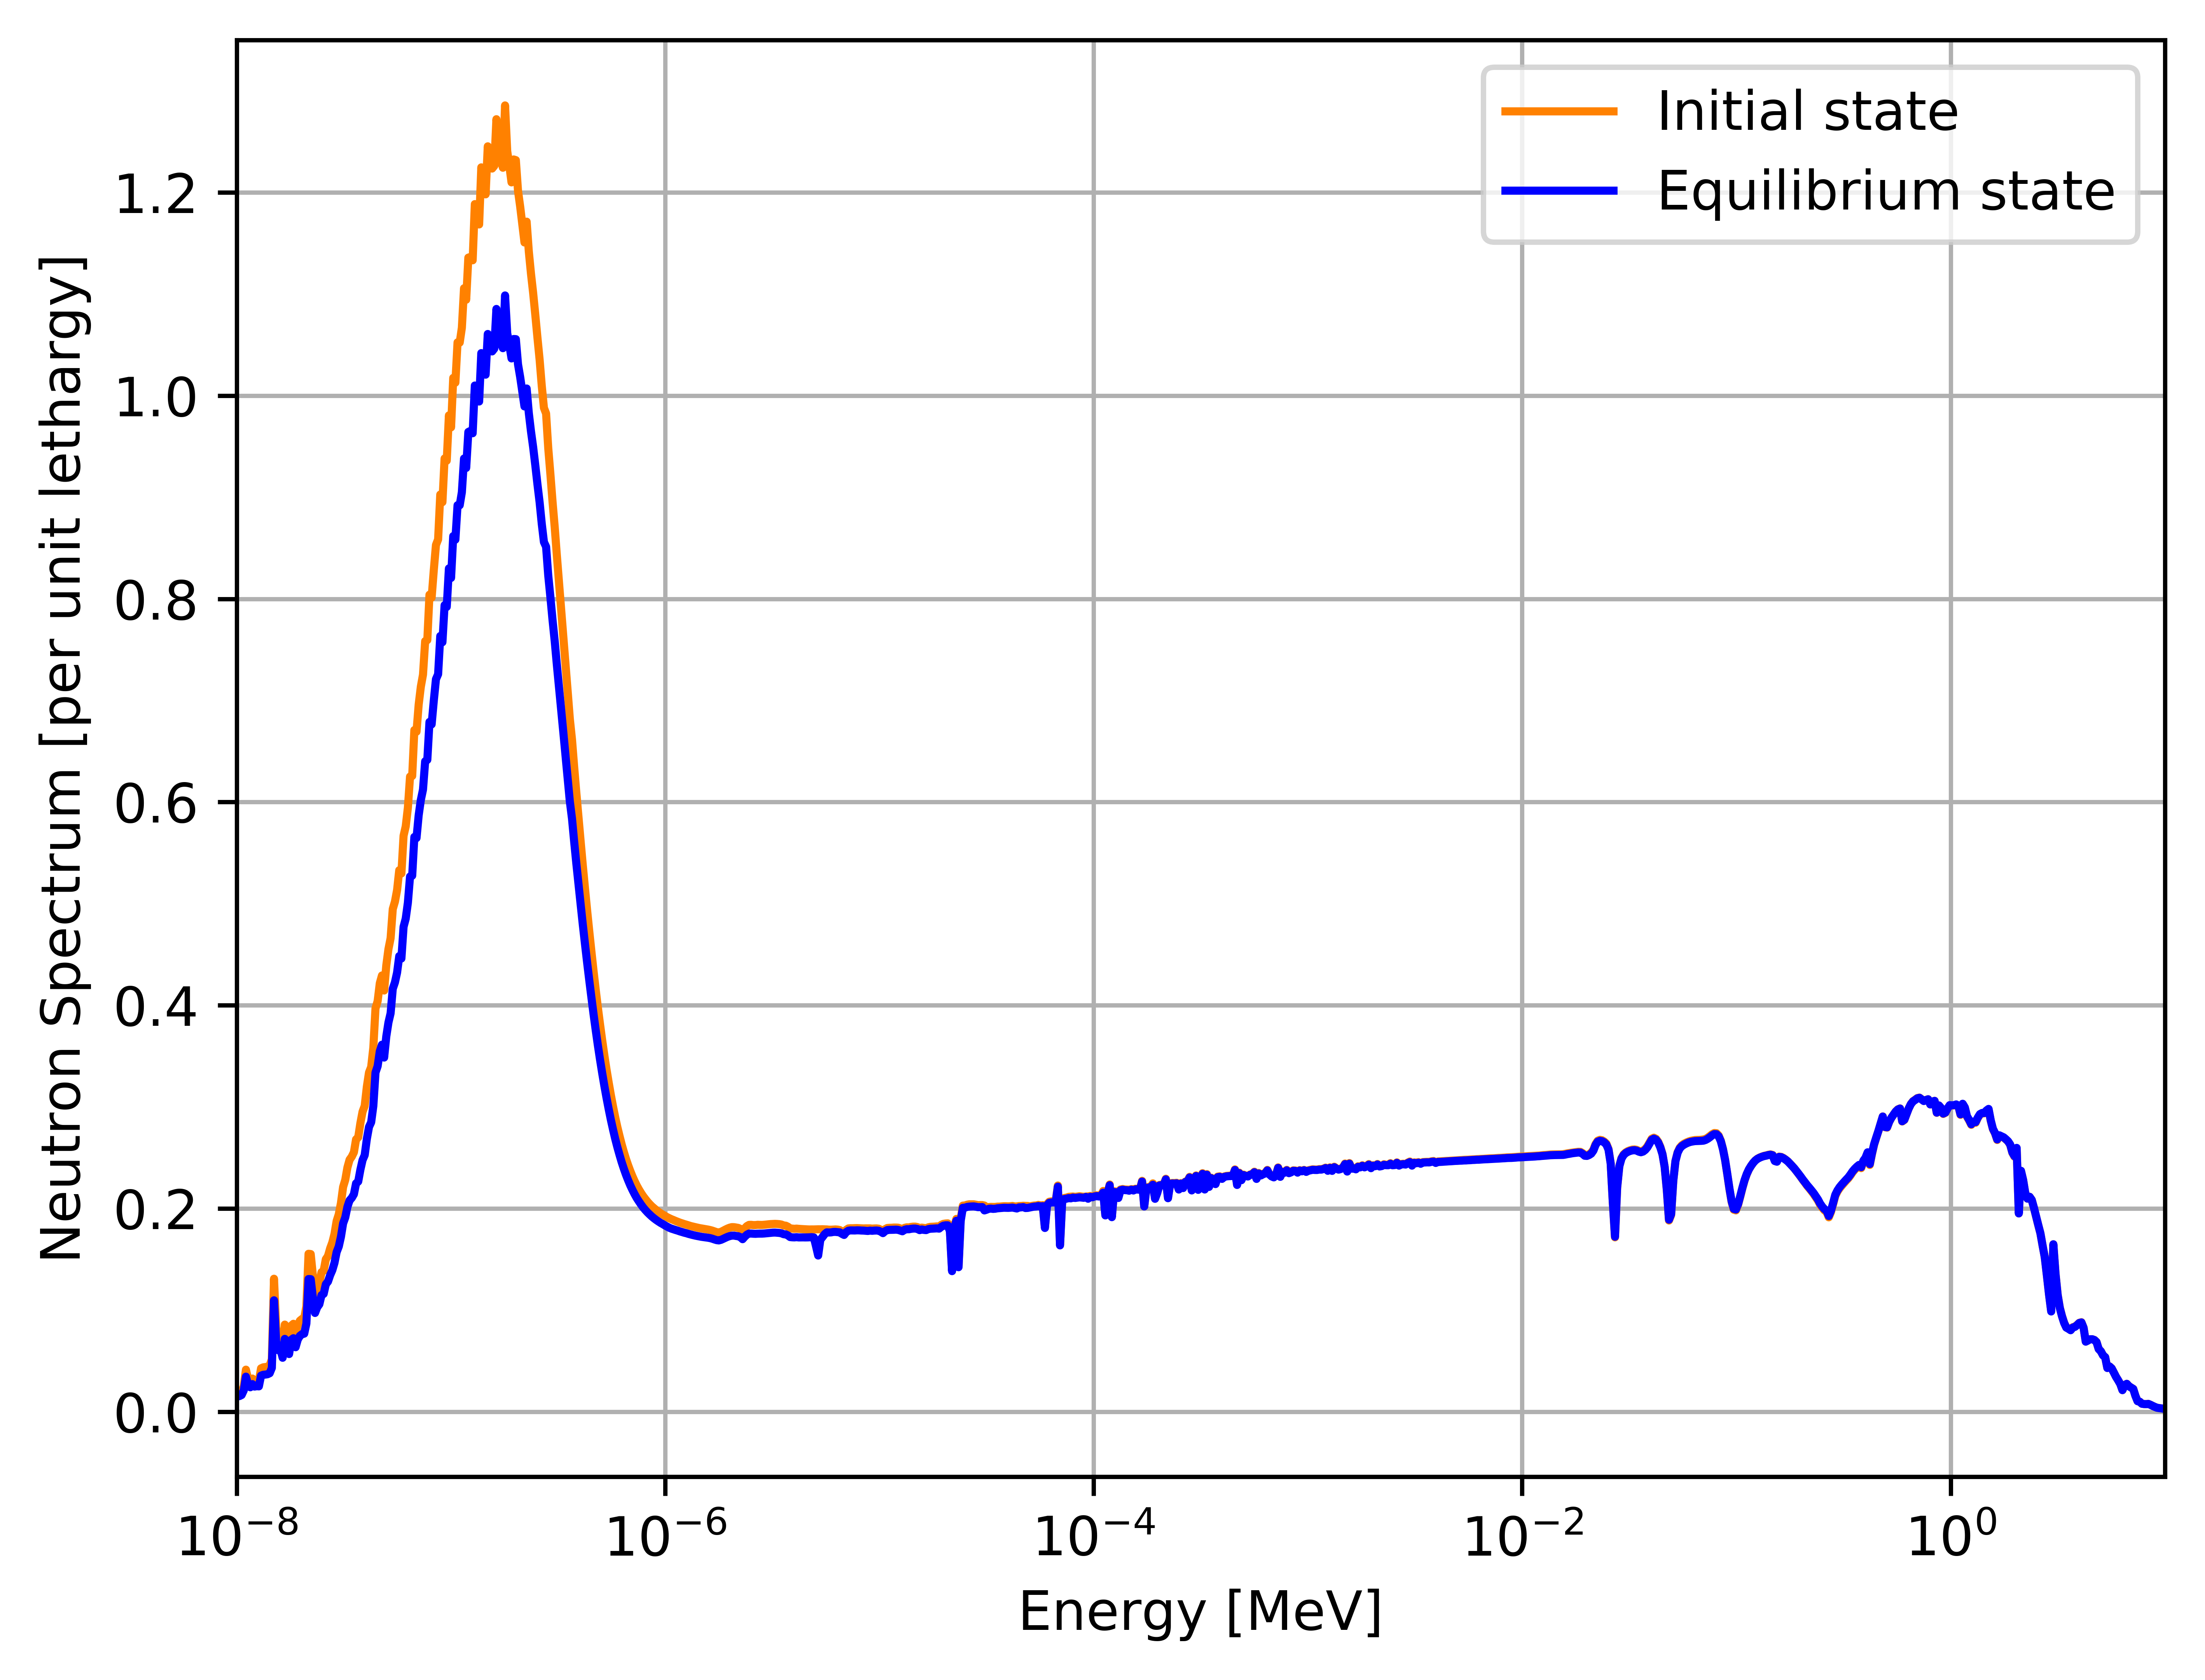
\includegraphics[width=\textwidth]{spectrum.png} 
  \caption{Neutron flux energy spectrum normalized by unit lethargy for initial and equilibrium fuel salt composition.}
    \vspace{-0.6em}
  \label{fig:spectrum}
\end{figure}
\FloatBarrier

Figure~\ref{fig:spectrum_zones_init}, \ref{fig:spectrum_zones_eq} shows that zone I produced much more thermal neutrons than zone II, indicating that the majority of fissions occured in the central part of the core. In the undermoderated zone II, the neutron energy spectrum is harder which leads to more capture of neutrons by $^{232}$Th and helps a achieve relatively high breeding ratio. Moreover, the (n,$\gamma$) resonance energy range in $^{232}$Th is from 10$^{-4}$ to 10$^{-2}$ MeV. Therefore, the moderator-to-fuel ratio for zone II was chosen to shift the neutron energy spectrum in this range. Furthermore, in the central core region (zone I), the neutron energy spectrum shifts to a harder spectrum over 20 years of reactor operation. In contrast, in the outer core region (zone II) a similar spectral shift takes place at a reduced scale. This resuls is in a good agreement with original ORNL report \cite{robertson_conceptual_1971} and most recent whole-core steady-state study \cite{park_whole_2015}.

It is important to obtain the epithermal and thermal spectra to produce $^{233}$U from $^{232}$Th because the radiative capture cross section of thorium decreases monotonically from $10^{-10}$ MeV to $10^{-5}$ MeV. Hardening the spectrum tends to significantly increase resonance absorption in thorium and decrease the absorptions in fissile and construction materials. Thus, a signficant amount fissile material will be needed to make the reactor critical. 

\begin{figure}[htp!] % replace 't' with 'b' to force it to 
  \centering
    \vspace{-0.3em}
  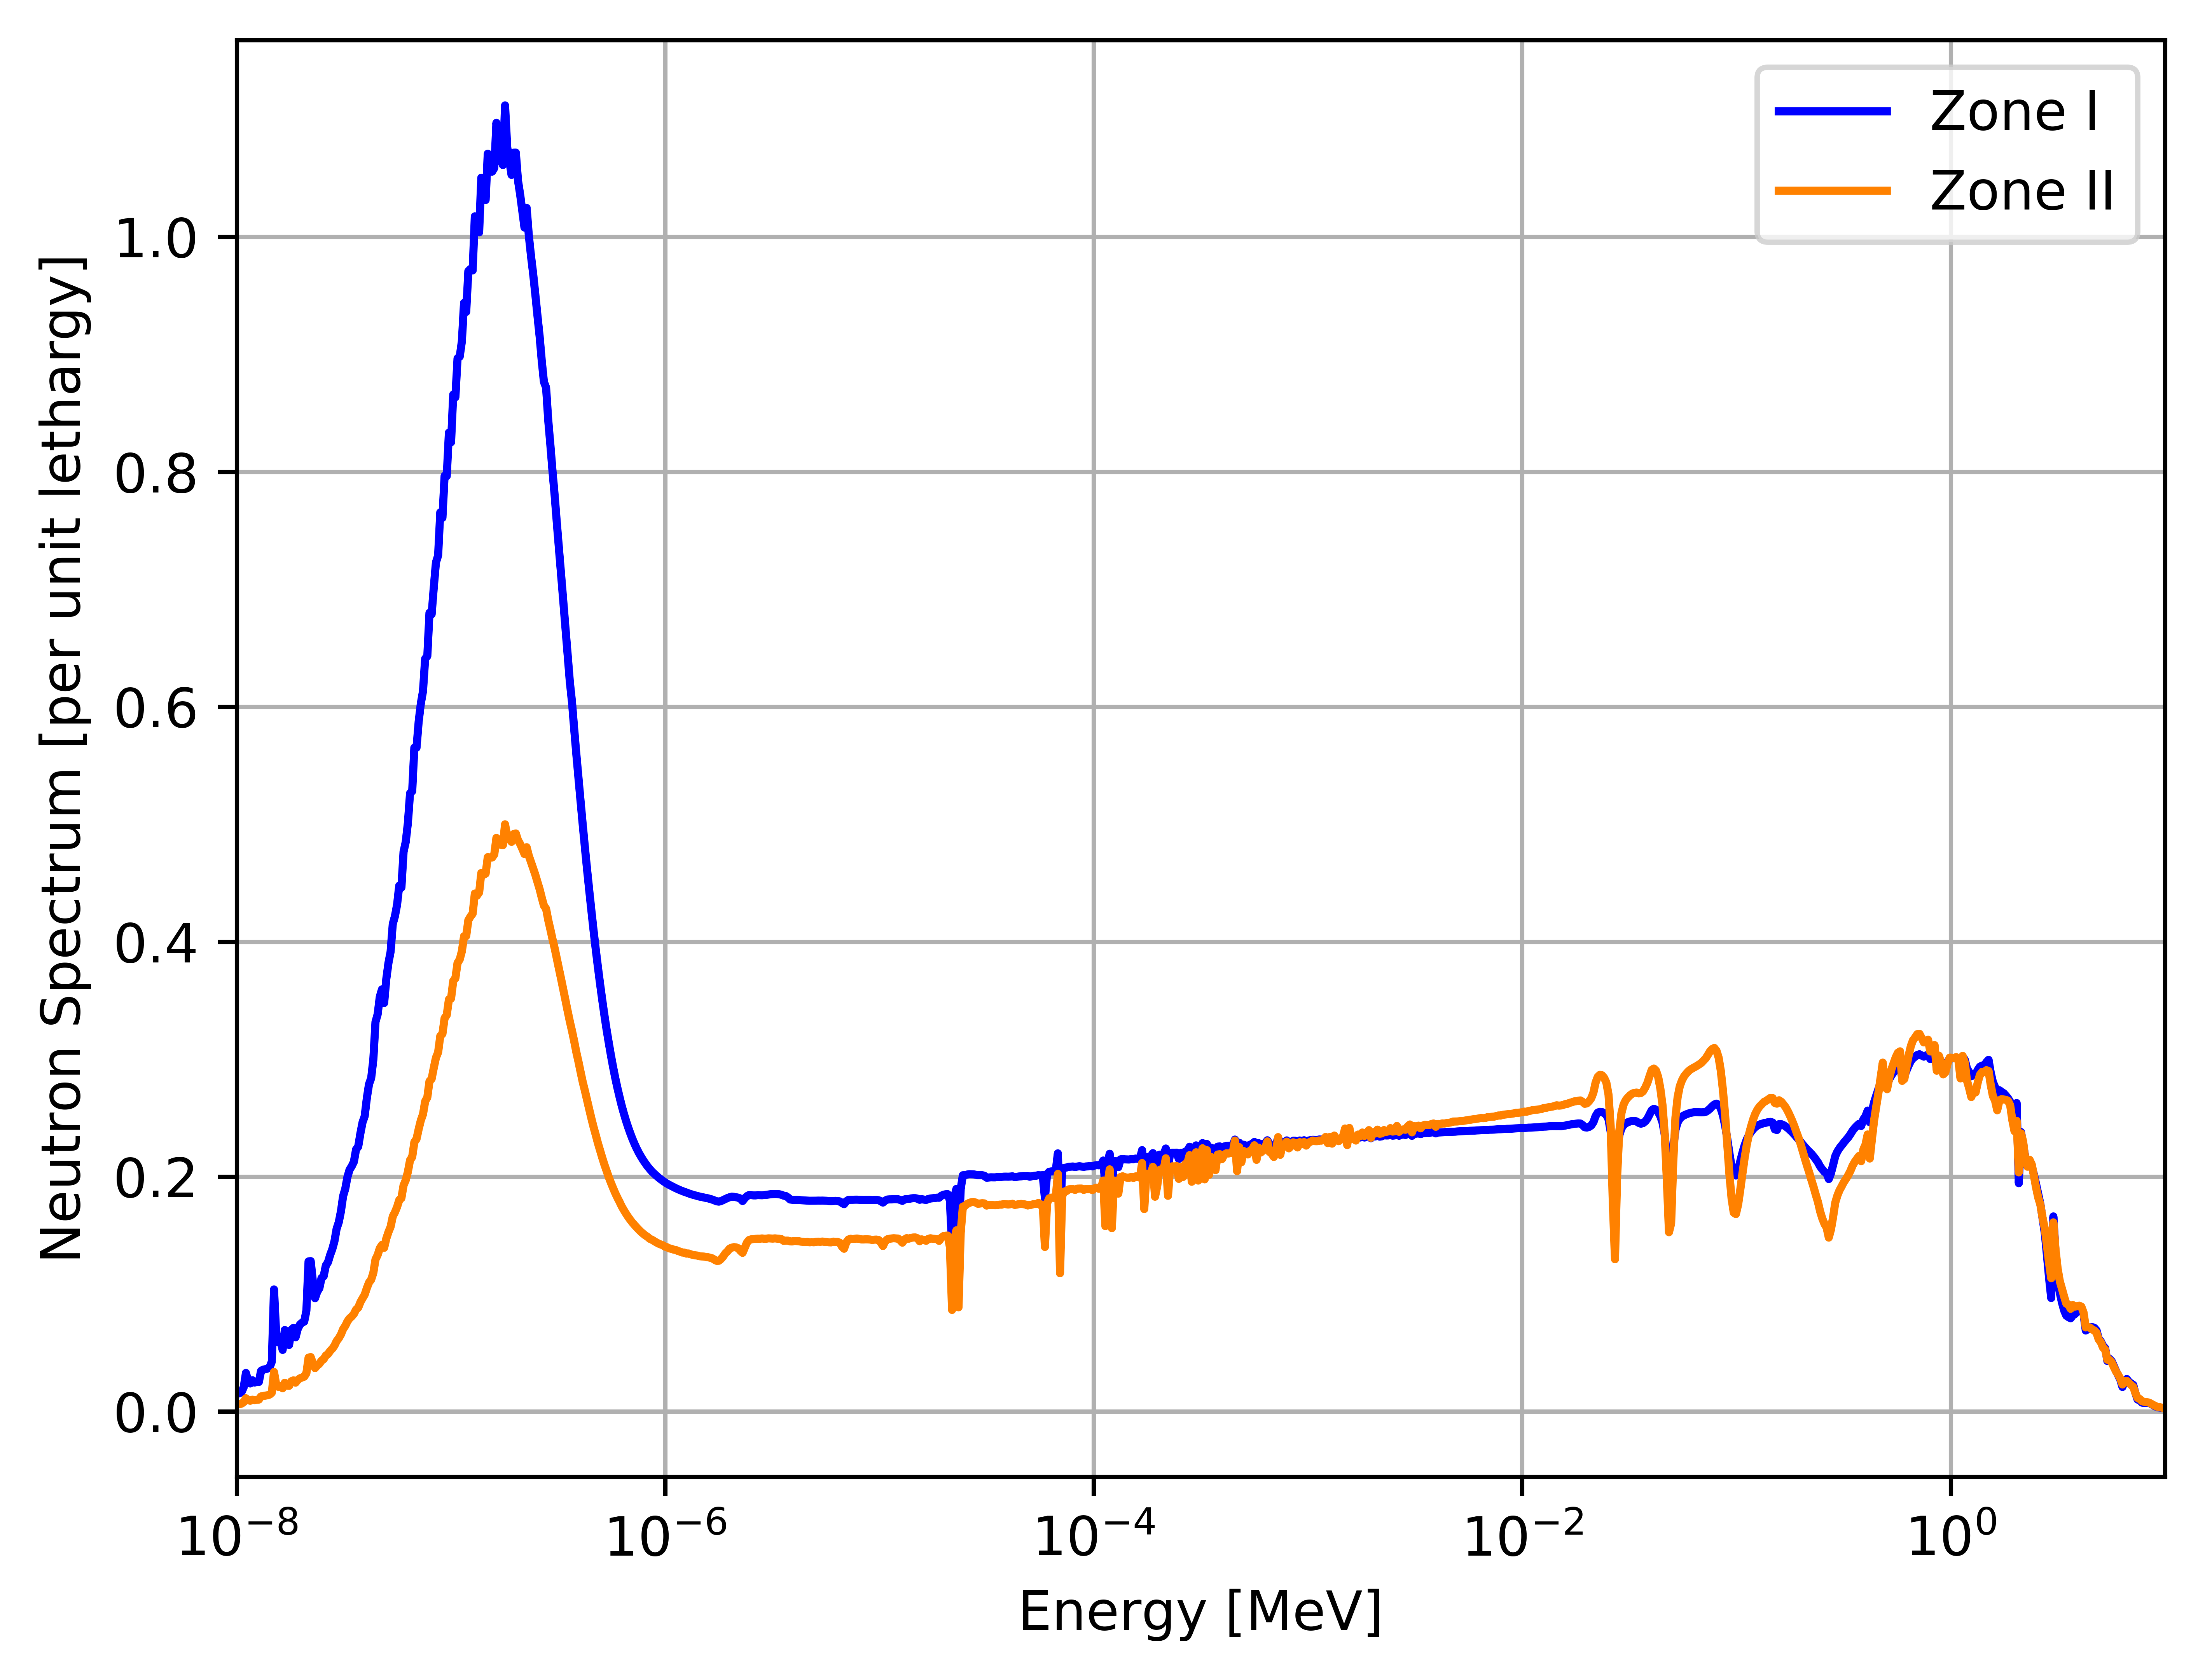
\includegraphics[width=\textwidth]{spectrum_zones_init.png} 
  \caption{Neutron flux energy spectrum in different core regions normalized by unit lethargy for the initial fuel salt composition.}
    \vspace{-1.6em}
  \label{fig:spectrum_zones_init}
\end{figure}
\begin{figure}[htp!] % replace 't' with 'b' to force it to 
  \centering
    \vspace{-0.3em}
  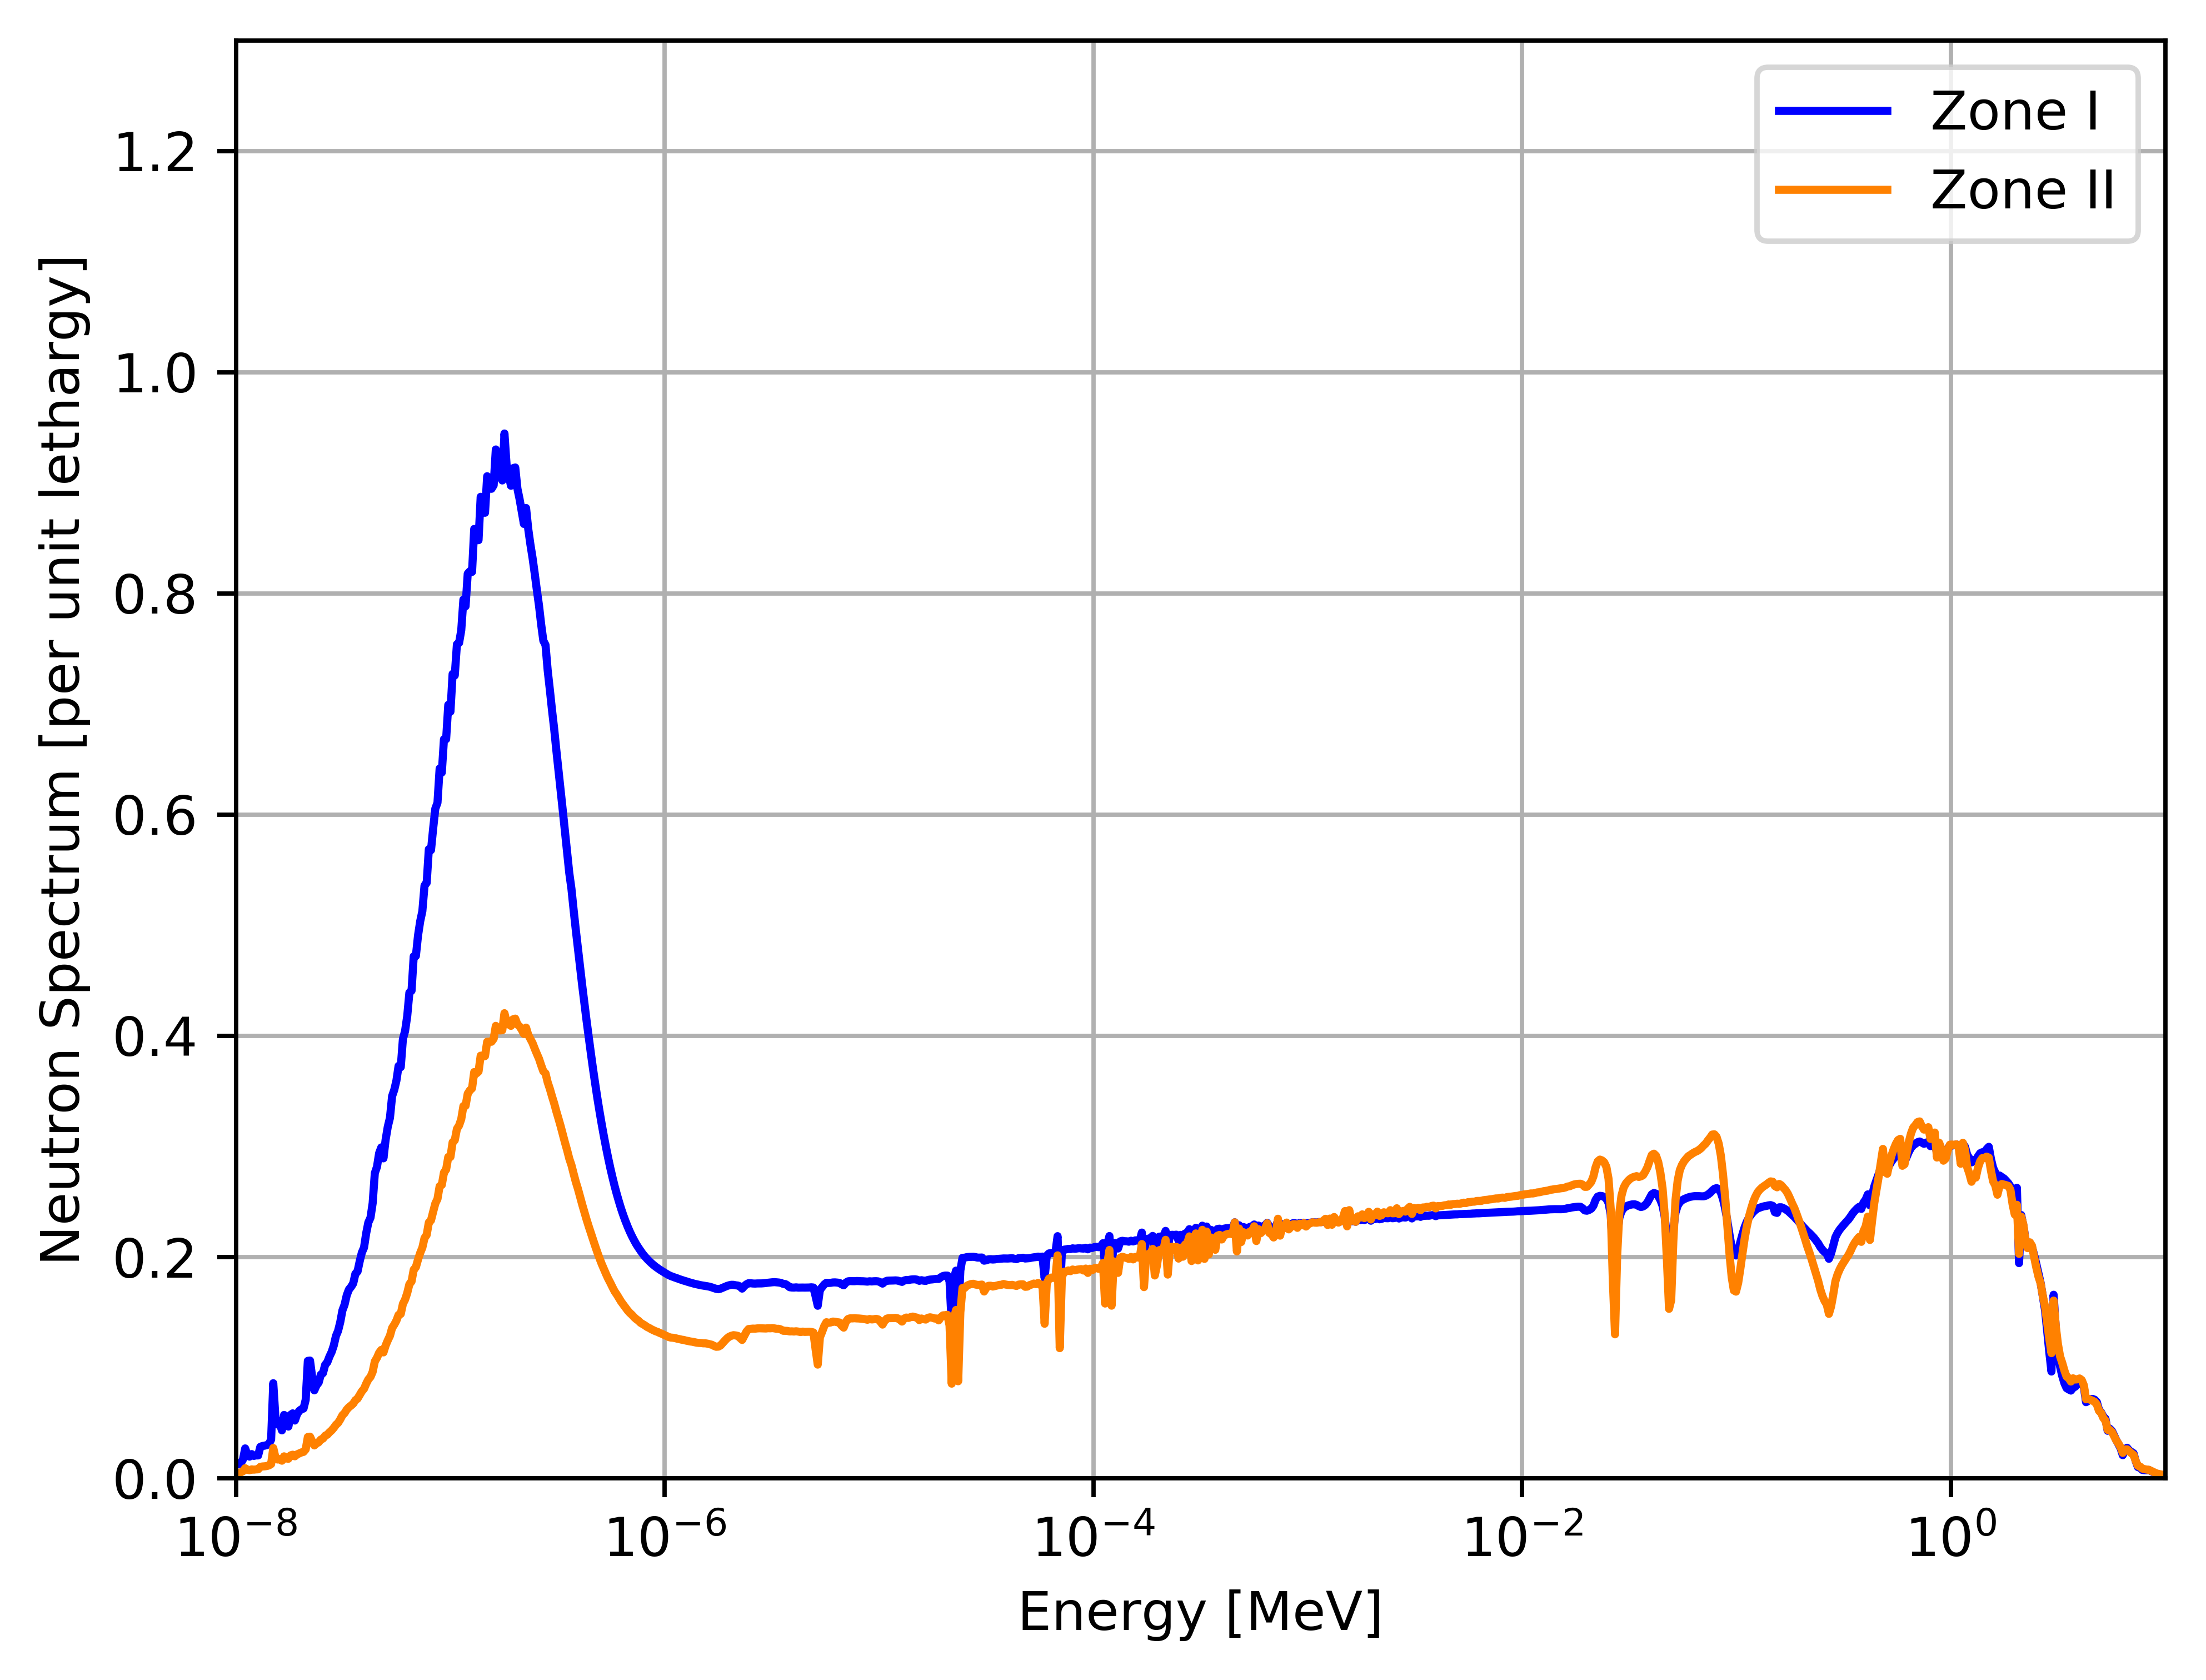
\includegraphics[width=\textwidth]{spectrum_zones_eq.png} 
  \caption{Neutron flux energy spectrum in different core regions normalized by unit lethargy for the equilibrium fuel salt composition.}
    \vspace{-1.6em}
  \label{fig:spectrum_zones_eq}
\end{figure}
\FloatBarrier

\section{Neutron flux}
Figure~\ref{fig:radial_flux} shows the radial distribution of fast and thermal neutron flux for both initial and equilibrium composition. The neutron flux has the same shape for both compositions but the equilibrium case has a harder spectrum. A significant spectral shift was observed for the central region of the core (zone I) when for the outer region (zone II) it is negligible for fast but notable for thermal neutrons. This neutron flux radial distribution is in a good agreement with original ORNL report \cite{robertson_conceptual_1971}. Overall, spectrum hardening during \gls{MSBR} operation should be carefully studied for designing the reactivity control system.

\begin{figure}[htp!] % replace 't' with 'b' to force it to 
  \centering
    \vspace{-0.3em}
  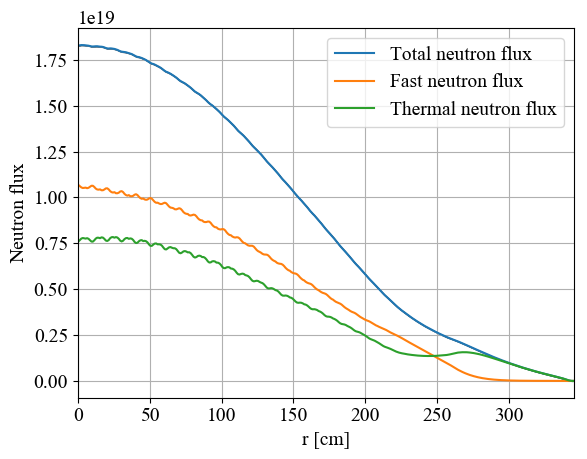
\includegraphics[width=\textwidth]{radial_flux.png} 
  \caption{Radial neutron flux distribution for initial and equilibrium fuel salt composition.}
    \vspace{-0.6em}
  \label{fig:radial_flux}
\end{figure}
\FloatBarrier

\section{Power and breeding distribution}
Table~\ref{tab:powgen_fraction} shows the power fraction in each zone for initial and equilibrium fuel composition. Figure~\ref{fig:pow_den} demonstrates the normalized power distribution of the \gls{MSBR} quater core at both states. For both the initial and equilibrium compositions, fission primarly occurs in the center of the core, namely zone I. The spectral shift during reactor operation results in different power fractions at startup and equilibrium, but most of the power is still generated in zone I. Figure~\ref{fig:breeding_den} shows the neutron capture reaction rate distribution for $^{232}$Th normalized by the total neutron flux for initial and equilibrium states. The distribution reflects the spatial distribution of $^{233}$Th production in the core. The thorium-232 then $\beta$-decays to $^{233}$Pa which is the precursor for $^{233}$U production. Accordingly, this characteristic represents the breeding distribution in the \gls{MSBR} core. Spectral shift does not cause significant changes in power nor in breeding distribution. Even after 20 years of operation, most of the power still is generated in zone I though the majority of $^{233}$Th is produced in zone II, which is in a good agreement with original ORNL report \cite{robertson_conceptual_1971}.

%%%%%%%%%%%%%%%%%%%%%%%%%%%%%%%%%%%%%%%%
\begin{table}[ht!]
  \centering
  \caption{Power generation fraction in each zone for initial and equilibrium state.}
\begin{tabular}{| m{0.22\textwidth} | m{0.22\textwidth} | m{0.22\textwidth} |} \hline
Core region      & Initial      & Equilibrium   \\ [3pt]\hline   
Zone I           & 97.91\%      & 98.12\%   \\ [3pt] \hline
Zone II          & 2.09\%       & 1.88\%   \\ [3pt] \hline
\end{tabular}
  \label{tab:powgen_fraction}
\end{table}
%%%%%%%%%%%%%%%%%%%%%%%%%%%%%%%%%%%%%%%%%%%%%%%%%%%%%%%%%%%%%%%%%%%%%%%%%%%%%%%%

\begin{figure}[htp!] % replace 't' with 'b' to force it to 
  \centering
    \vspace{-0.3em}
  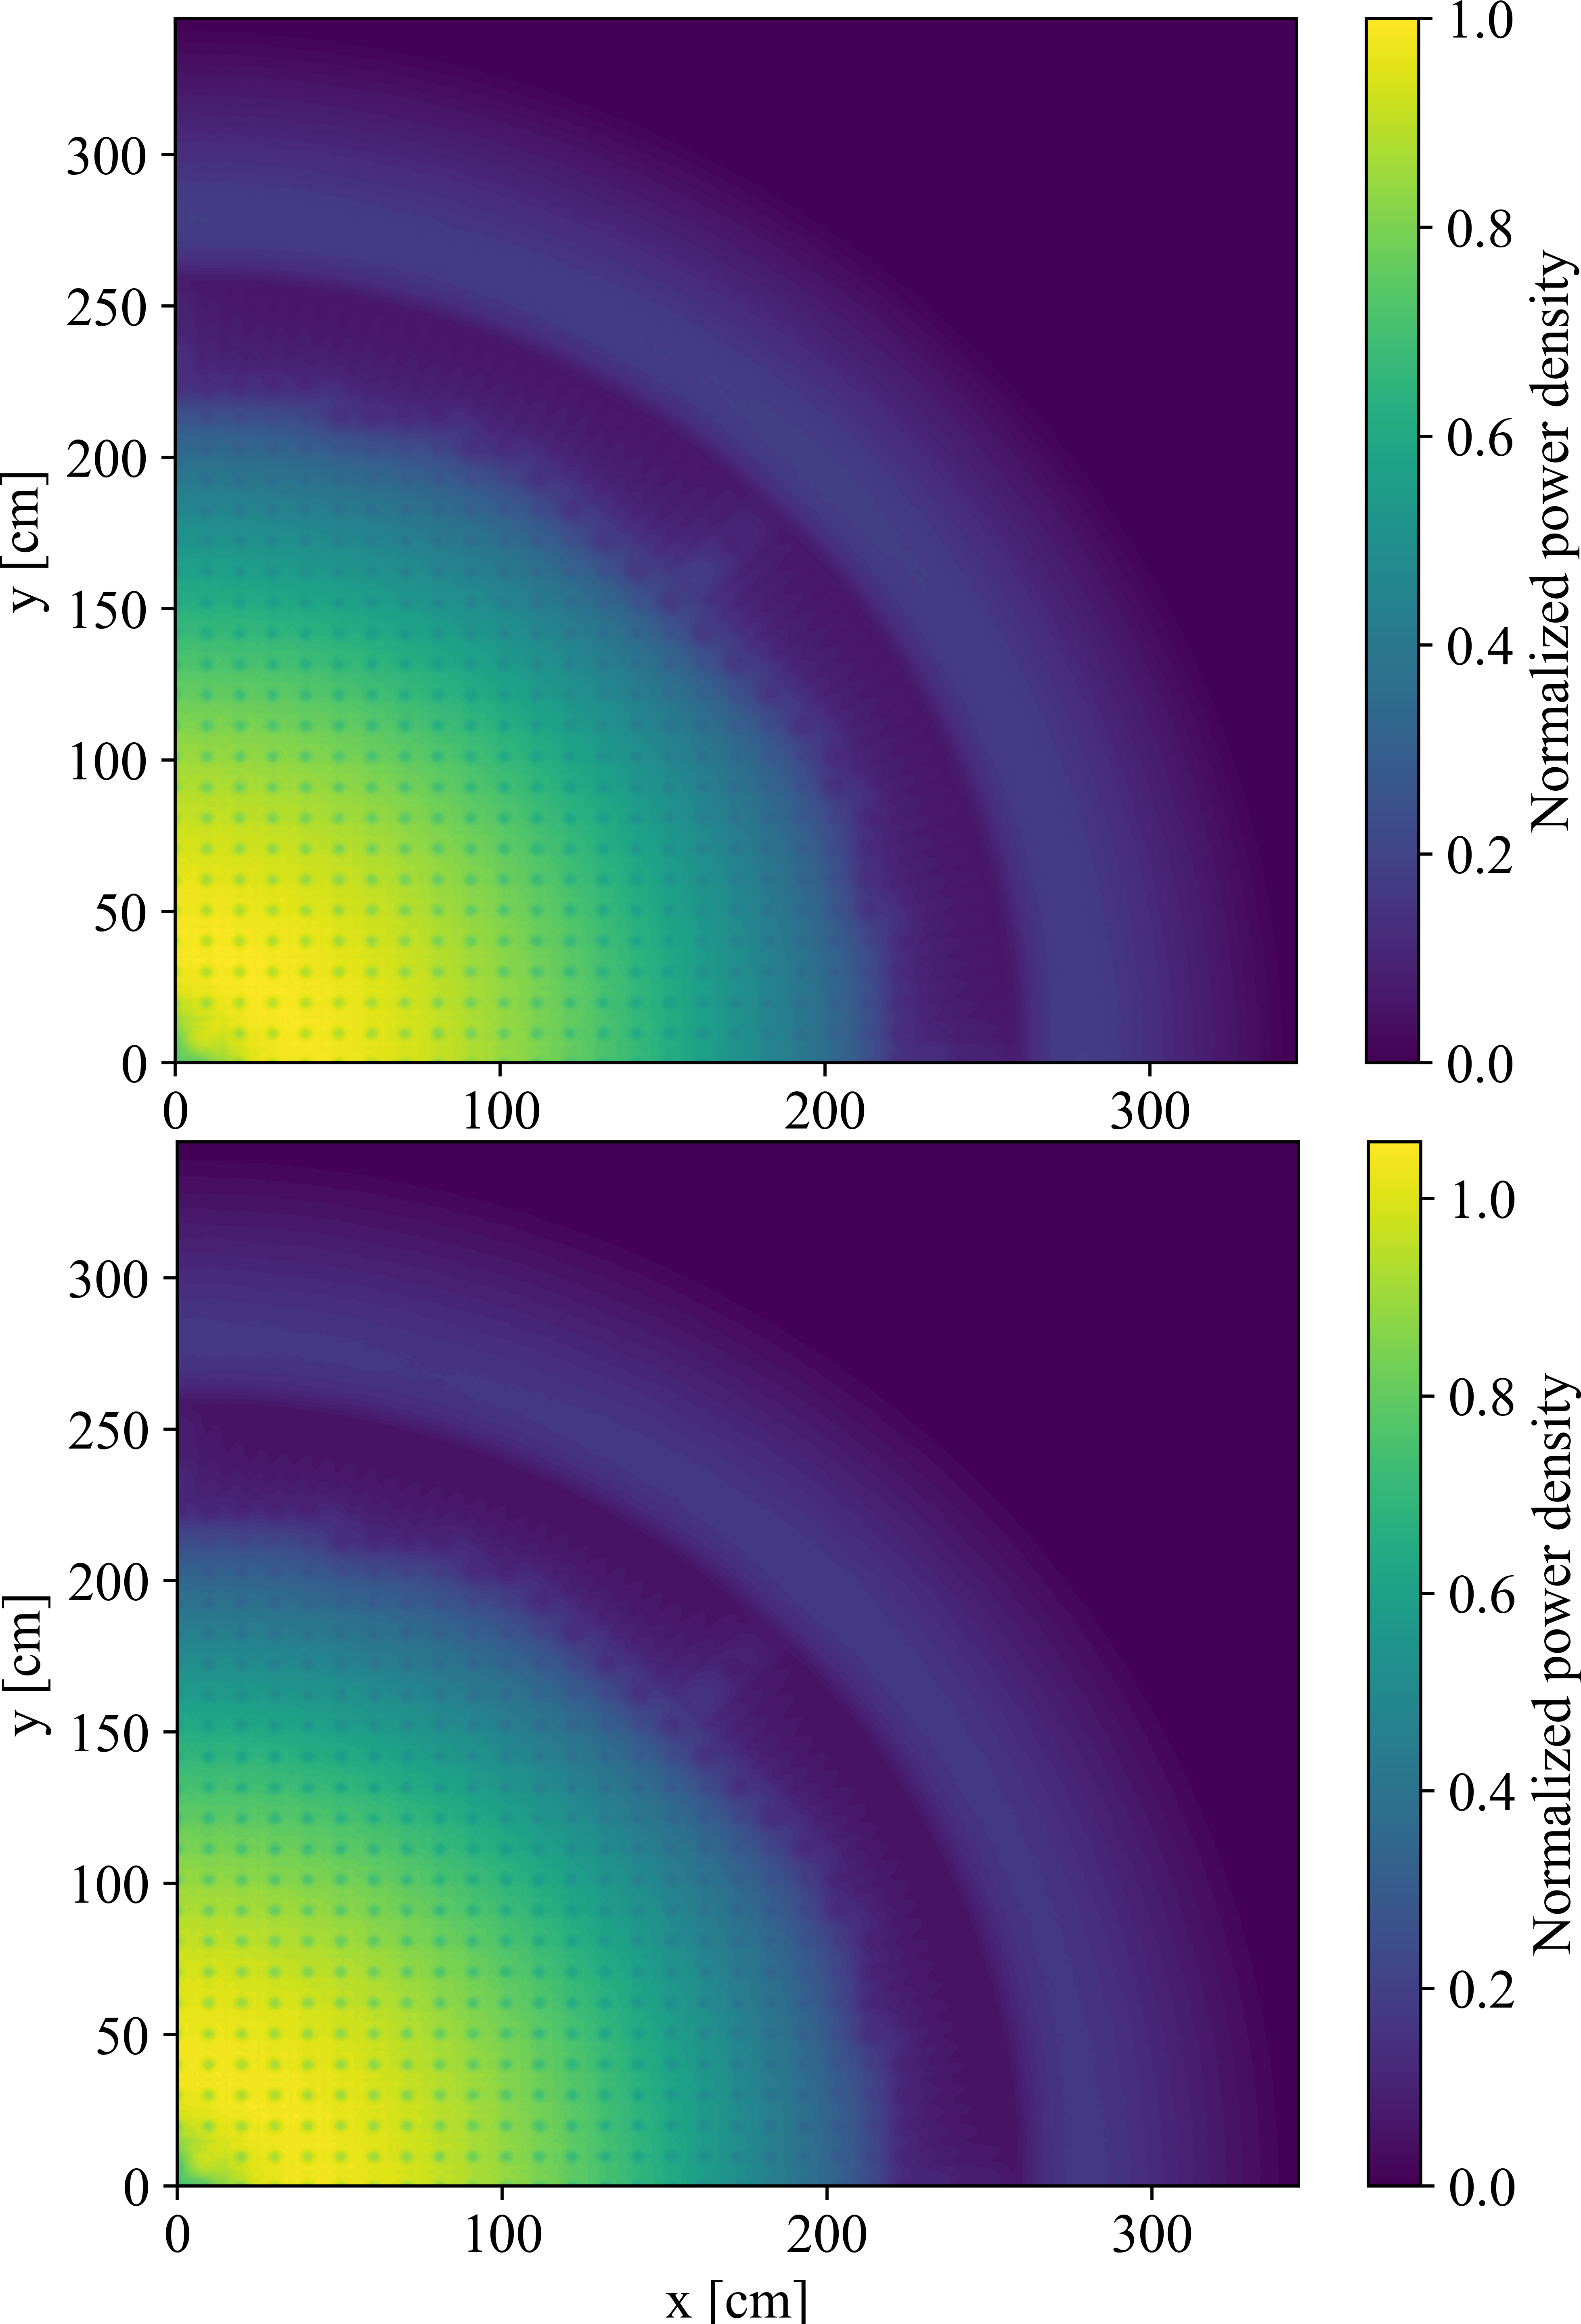
\includegraphics[width=\textwidth]{power_distribution.png} 
  \caption{Normalized power density for initial (top) and equilibrium (bottom) fuel salt composition.}
    \vspace{-0.6em}
  \label{fig:pow_den}
\end{figure}
\FloatBarrier

\begin{figure}[htp!] % replace 't' with 'b' to force it to 
  \centering
    \vspace{-0.3em}
  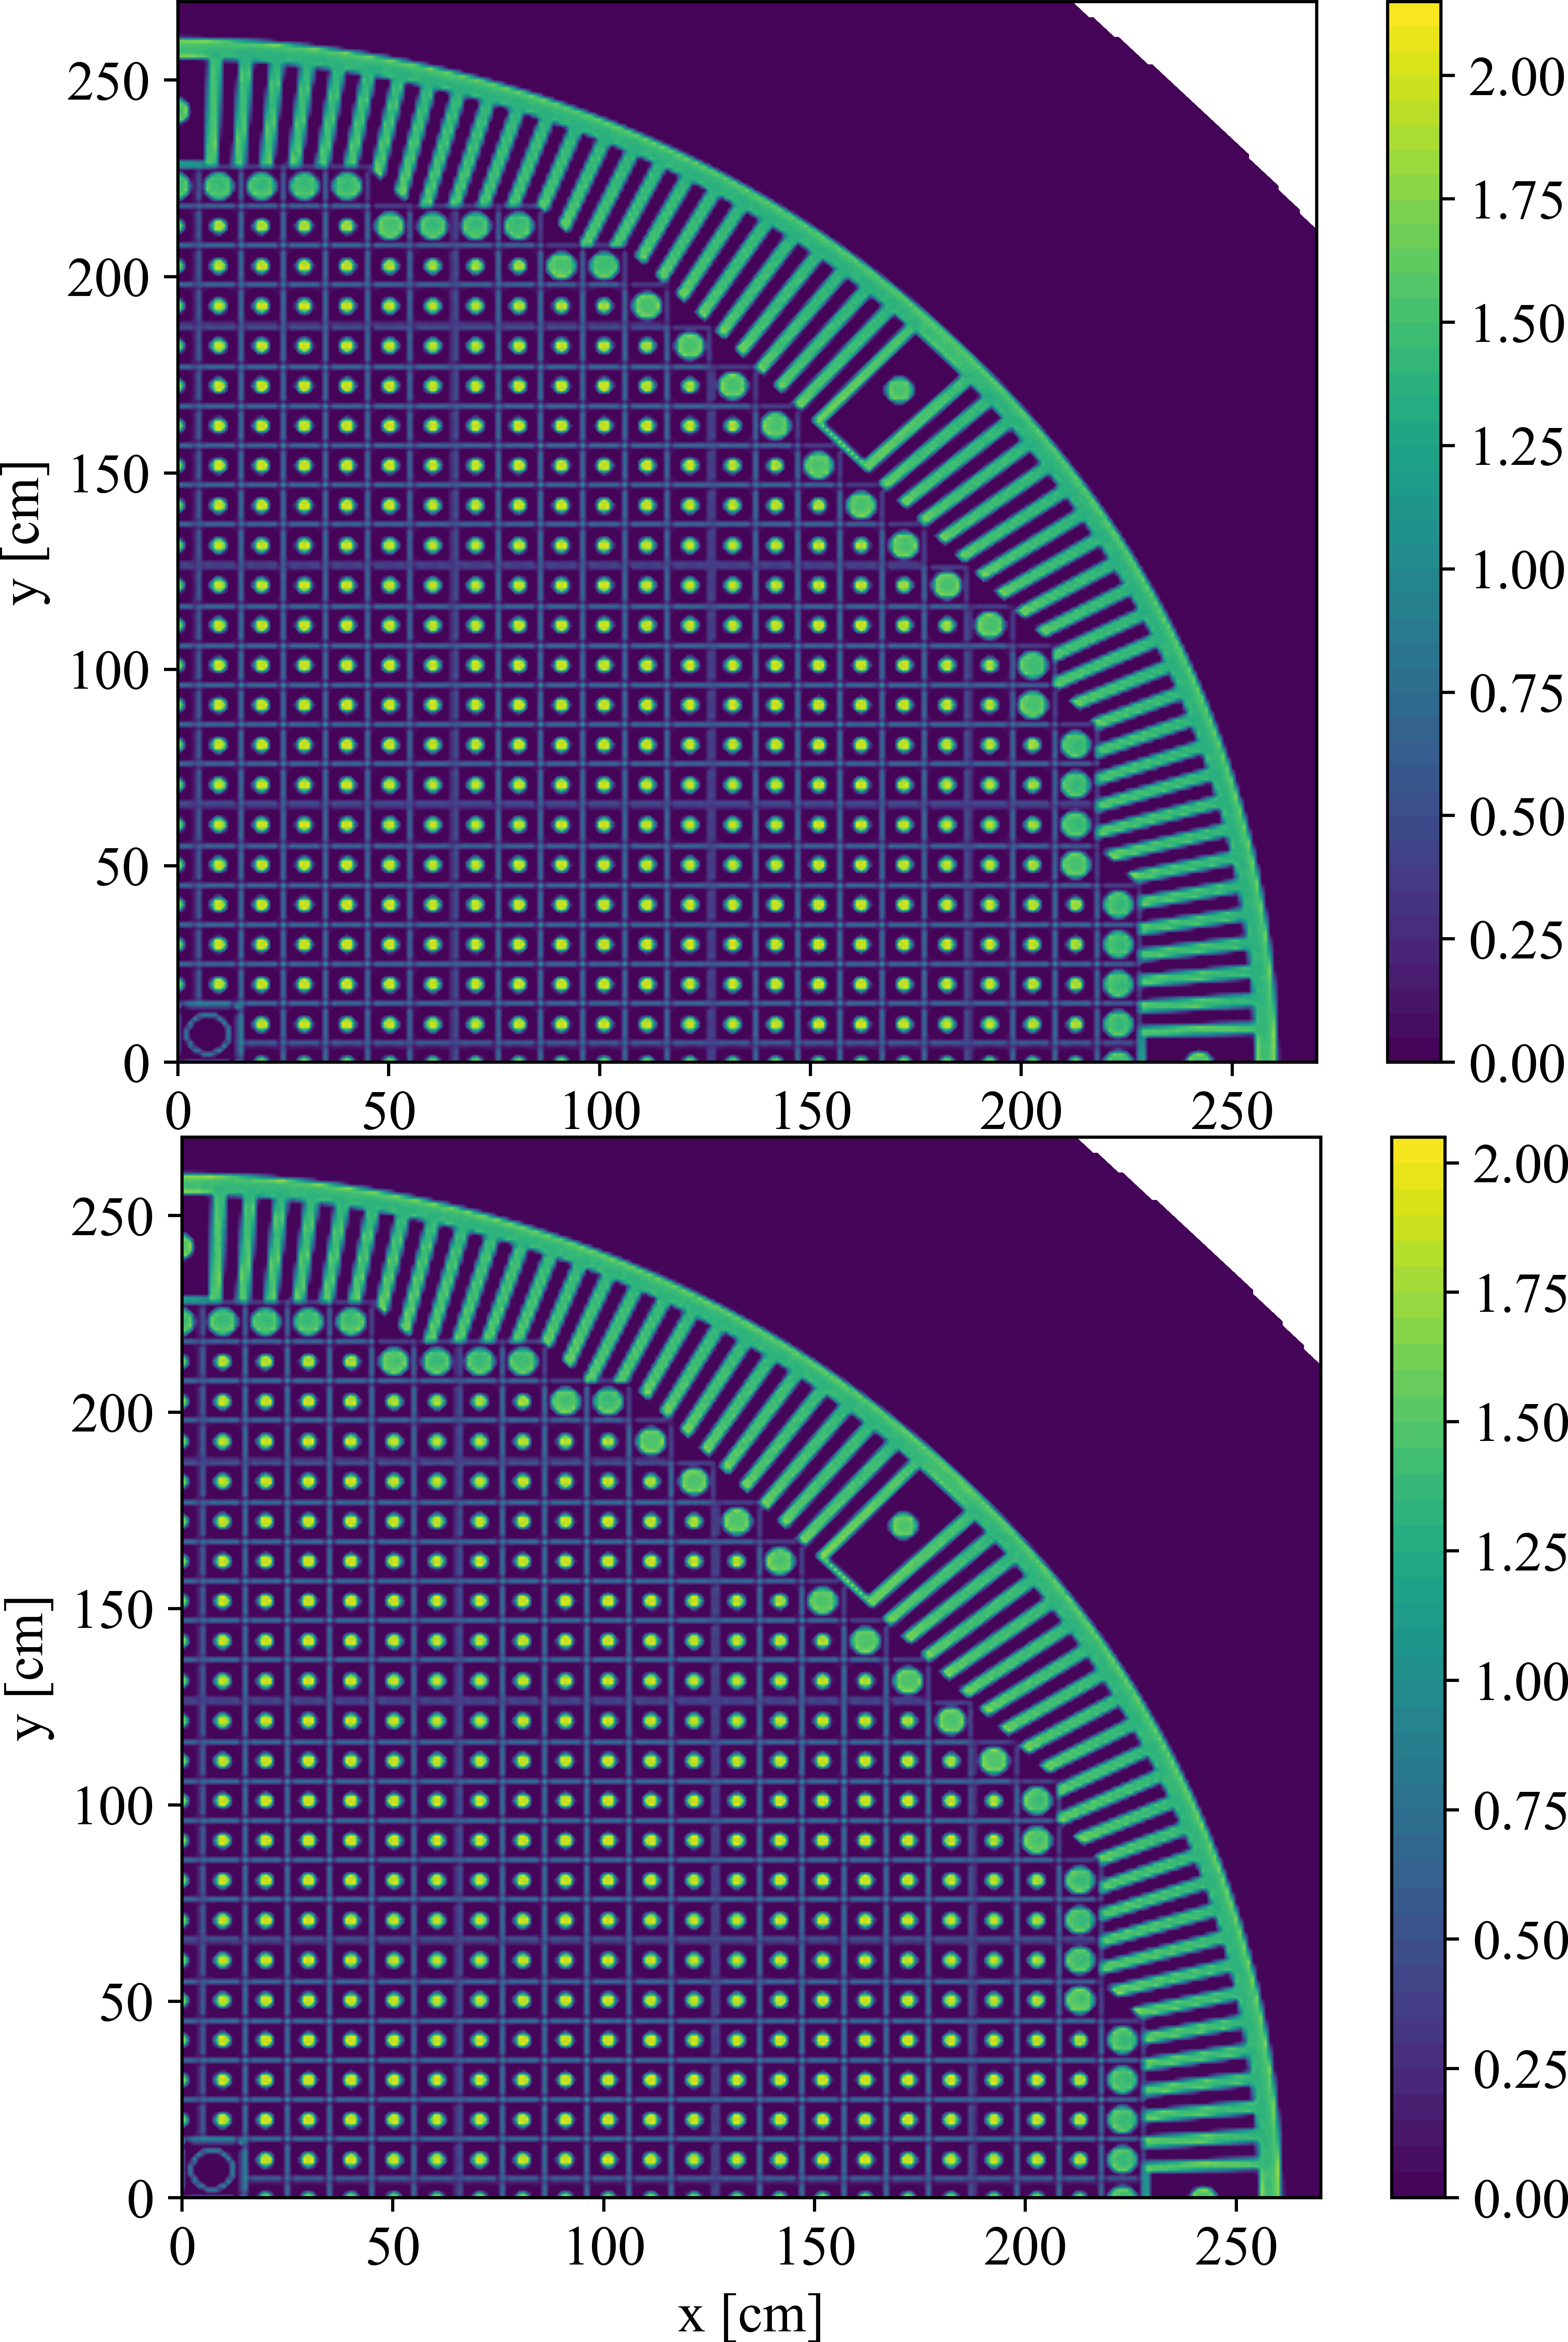
\includegraphics[width=\textwidth]{breeding_distribution.png} 
  \caption{$^{232}$Th neutron capture reaction rate normalized by total flux for initial (top) and equilibrium (bottom) fuel salt composition.}
    \vspace{-0.6em}
  \label{fig:breeding_den}
\end{figure}
\FloatBarrier

\section{Temperature coefficient of reactivity}
Table~\ref{tab:tcoef} summarizes temperature effects on reactivity calculated in this work for both initial and equilibrium fuel composition, and compared with original \gls{ORNL} report data \cite{robertson_conceptual_1971}. Uncertainty for each temperature coefficient also appears in Table~\ref{tab:tcoef}. The main physical principle underlying the reactor temperature feedback is an expansion of matterial that is heated. When the fuel salt temperature increases, the density of the salt decreases, but at the same time, the total volume of fuel salt in the core remains constant because it is bounded by the graphite. When the graphite temperature increases, the density of graphite decreases creating additional space for fuel salt. To determine temperature coefficients, the cross section temperatures for fuel and moderator were changed from 900K to 1000K. Three different cases were considered:
\begin{enumerate}
  \item Temperature of fuel salt rising from 900K to 1000K.
  \item Temperature of graphite rising from 900K to 1000K.
  \item Whole reactor temperature rising from 900K to 1000K.
\end{enumerate}

%%%%%%%%%%%%%%%%%%%%%%%%%%%%%%%%%%%%%%%%
\begin{table}[ht!]
  \centering
  \caption{Temperature coefficients of reactivity for initial and equilibrium state.}
\begin{tabular}{| m{0.22\textwidth} | m{0.22\textwidth} | m{0.22\textwidth} | m{0.20\textwidth} |} \hline
   Reactivity coefficient [pcm/K]  & Initial      & Equilibrium  & Reference \cite{robertson_conceptual_1971} \\ [5pt]\hline   
Fuel salt        & $-3.22\pm0.044$ & $-1.53\pm0.046$ & $-3.22$  \\ [3pt] \hline
Moderator        & $+1.61\pm0.044$ & $+0.97\pm0.046$ & $+2.35$  \\ [3pt] \hline
Total            & $-3.1\pm0.04$   & $-0.97\pm0.046$ & $-0.87$  \\ [3pt] \hline
\end{tabular}
  \label{tab:tcoef}
\end{table}
%%%%%%%%%%%%%%%%%%%%%%%%%%%%%%%%%%%%%%%%%%%%%%%%%%%%%%%%%%%%%%%%%%%%%%%%%%%%%%%%
In the first case, changes in the fuel temperature only impact fuel density. In this case, the geometry is unchanged because the fuel is a liquid. However, when the moderator heats up, both the density and the geometry change due to thermal expansion of the solid graphite blocks and reflector. Accordingly, the new graphite density was calculated using a linear temperature expansion coefficient of 1.3$\times10^{-6}$1/K \cite{robertson_conceptual_1971}. A new geometry input was created based on this information.

The fuel temperature coefficient (FTC) is negative for both initial and equilibrium fuel compositon due to thermal Doppler broadening of the resonance capture cross sections in the thorium and is in a good agreement with earlier research \cite{robertson_conceptual_1971,park_whole_2015}. The moderator temperature coefficient (MTC) is positive for startup composition and decreases during reactor operation because of spectrum hardening with fuel depletion. Finally, the total temperature coefficient of reactivity is negative for both cases, but decreases during reactor operation due to spectral shift. In summary, even after 20 years of operation the total temperature coefficient of reactivity is relatively large and negative during reactor operation, despite positive MTC, and affords excellent reactor stability and control.

\section{Reactivity control system rod worth}
Table~\ref{tab:rod_worth} summarizes the reactivity control system worth. During normal operation the control (graphite) rods are fully inserted, and the safety (B$_4$C) rods are fully withdrawn. To insert negative reactivity into the core, the graphite rods are gradually withdrawn from the core. In an accident, the safety rods would fall down into the core. The integral rod worths were calculated for various positions to separately estimate control (graphite) rod, safety (B$_4$C) rod, and the whole reactivity control system worth. Control rod integral worth is approximately 28 cents and stays almost constant during reactor operation. The safety rod integral worth decreases by  16.2\% during 20 years of operation because of neutron spectrum hardening and absorber accumulation in proximity to reactivity control system rods. This 16\% decline in control system worth should be taken into account in \gls{MSBR} accident analysis and safety justification.

%%%%%%%%%%%%%%%%%%%%%%%%%%%%%%%%%%%%%%%%
\begin{table}[hb!]
  \centering
  \caption{Control system rod worth for initial and equilibrium fuel composition.}
\begin{tabular}{| m{0.60\textwidth} | m{0.15\textwidth} | m{0.15\textwidth} |} \hline
\qquad\qquad Reactivity parameter  & \quad Initial      & \enspace Equilibrium      \\[3pt] \hline   
Control (graphite) rod integral worth (cents)               & $\ 28.2\pm0.8$     & $\ 29.0\pm0.8$ \\[3pt]  \hline 
Safety (B$_4$C) rod integral worth (cents)                  & $251.8\pm0.8$    & $211.0\pm0.8$  \\[3pt]  \hline
Total reactivity control system worth (cents)               & $505.8\pm0.7$    & $424.9\pm0.8$ \\[3pt] \hline
\end{tabular}
  \label{tab:rod_worth}
\end{table}
%%%%%%%%%%%%%%%%%%%%%%%%%%%%%%%%%%%%%%%%%%%%%%%%%%%%%%%%%%%%%%%%%%%%%%%%%%%%%%%%

\section{Six Factor Analysis}
The effective multiplication factor could be expressed using formula:
\begin{align*}
k_{eff} = k_{inf} P_f  P_t \\
 = \eta \epsilon p f P_f P_t
\end{align*}

%%%%%%%%%%%%%%%%%%%%%%%%%%%%%%%%%%%%%%%%
\begin{table}[ht!]
  \centering
  \caption{Six factors for the full-core \gls{MSBR} model for initial and equilibrium fuel composition.}
\begin{tabular}{| m{0.44\textwidth} | m{0.22\textwidth} | m{0.22\textwidth} |} \hline
	   \qquad\qquad\qquad Factors  & \qquad Initial      & \qquad Equilibrium   \\ [3pt]\hline   
Neutron reproduction factor ($\eta$)     & $1.3960\pm.000052$     & $1.3778\pm.00005$ \\ [3pt] \hline
Thermal utilization factor (f)           & $0.9670\pm.000011$     & $0.9706\pm.00001$ \\ [3pt] \hline
Resonance escape probability (p)         & $0.6044\pm.000039$     & $0.5761\pm.00004$ \\ [3pt] \hline
Fast fission factor ($\epsilon$)         & $1.3421\pm.000040$     & $1.3609\pm.00004$ \\ [3pt] \hline
Fast non-leakage probability (P$_f$)     & $0.9999\pm.000004$     & $0.9999\pm.000004$ \\ [3pt] \hline
Thermal non-leakage probability (P$_t$)  & $0.9894\pm.000005$     & $0.9912\pm.00005$ \\ [3pt] \hline
\end{tabular}
  \label{tab:six_factor}
\end{table}
%%%%%%%%%%%%%%%%%%%%%%%%%%%%%%%%%%%%%%%%%%%%%%%%%%%%%%%%%%%%%%%%%%%%%%%%%%%%%%%%

Table~\ref{tab:six_factor} summarizes the six factors for both initial and equilibrium fuel salt composition. The non-leakage probability for both fast and thermal neutrons does not change during reactor operation because these values are not largely affected by the neutron spectrum shift. In contrast, neutron reproduction factor ($\eta$), resonance escape probability (p), and fast fission factor ($\epsilon$) are considerably different between startup and equilibrium. As indicated in Figure~\ref{fig:spectrum} the neutron spectrum is softer for the initial state. Neutron spectrum hardening causes the fast fission to increase throught the core lifetime. The opposite is true for the resonance escape probability. Finally, the neutron reproduction factor decreases during reactor operation due to accumulation of fissile plutonium isotopes.

\section{Thorium refill rate}
As was mentioned in Chapter 4, the only external feed material flow for this \gls{MSBR} reprocessing scheme is $^{232}$Th. Figure~\ref{fig:th_refill} shows the $^{232}$Th feed rate calculated for 20 years of reactor operation. Figure~\ref{fig:th_refill_spike} shows the large spikes up to 36 kg/day in a thorium consumption every 3435 days. This is required due to batch-wise removal of strong absorbers (Rb, Sr, Cs, Ba). The corresponding effective multiplication factor increase (Figure~\ref{fig:keff}) and breeding intensification leads to additional $^{232}$Th consumption. As indicated in Figure~\ref{fig:th_refill}, the average thorium feed rate increases during the first 500 days of operation and than steadily decreases due to spectrum hardening and accumulation of absorbers in the core. As a result, the average $^{232}$Th feed rate over 20 years of operation is about 2.39 kg/day. This results is in a good agreement with a recent online reprocessing study by \gls{ORNL} \cite{betzler_molten_2017} which reported thorium-232 refill rate for single-cell online reprocessing of 2.45 kg/day.

\begin{figure}[htp!] % replace 't' with 'b' to force it to 
  \centering
    \vspace{-0.3em}
  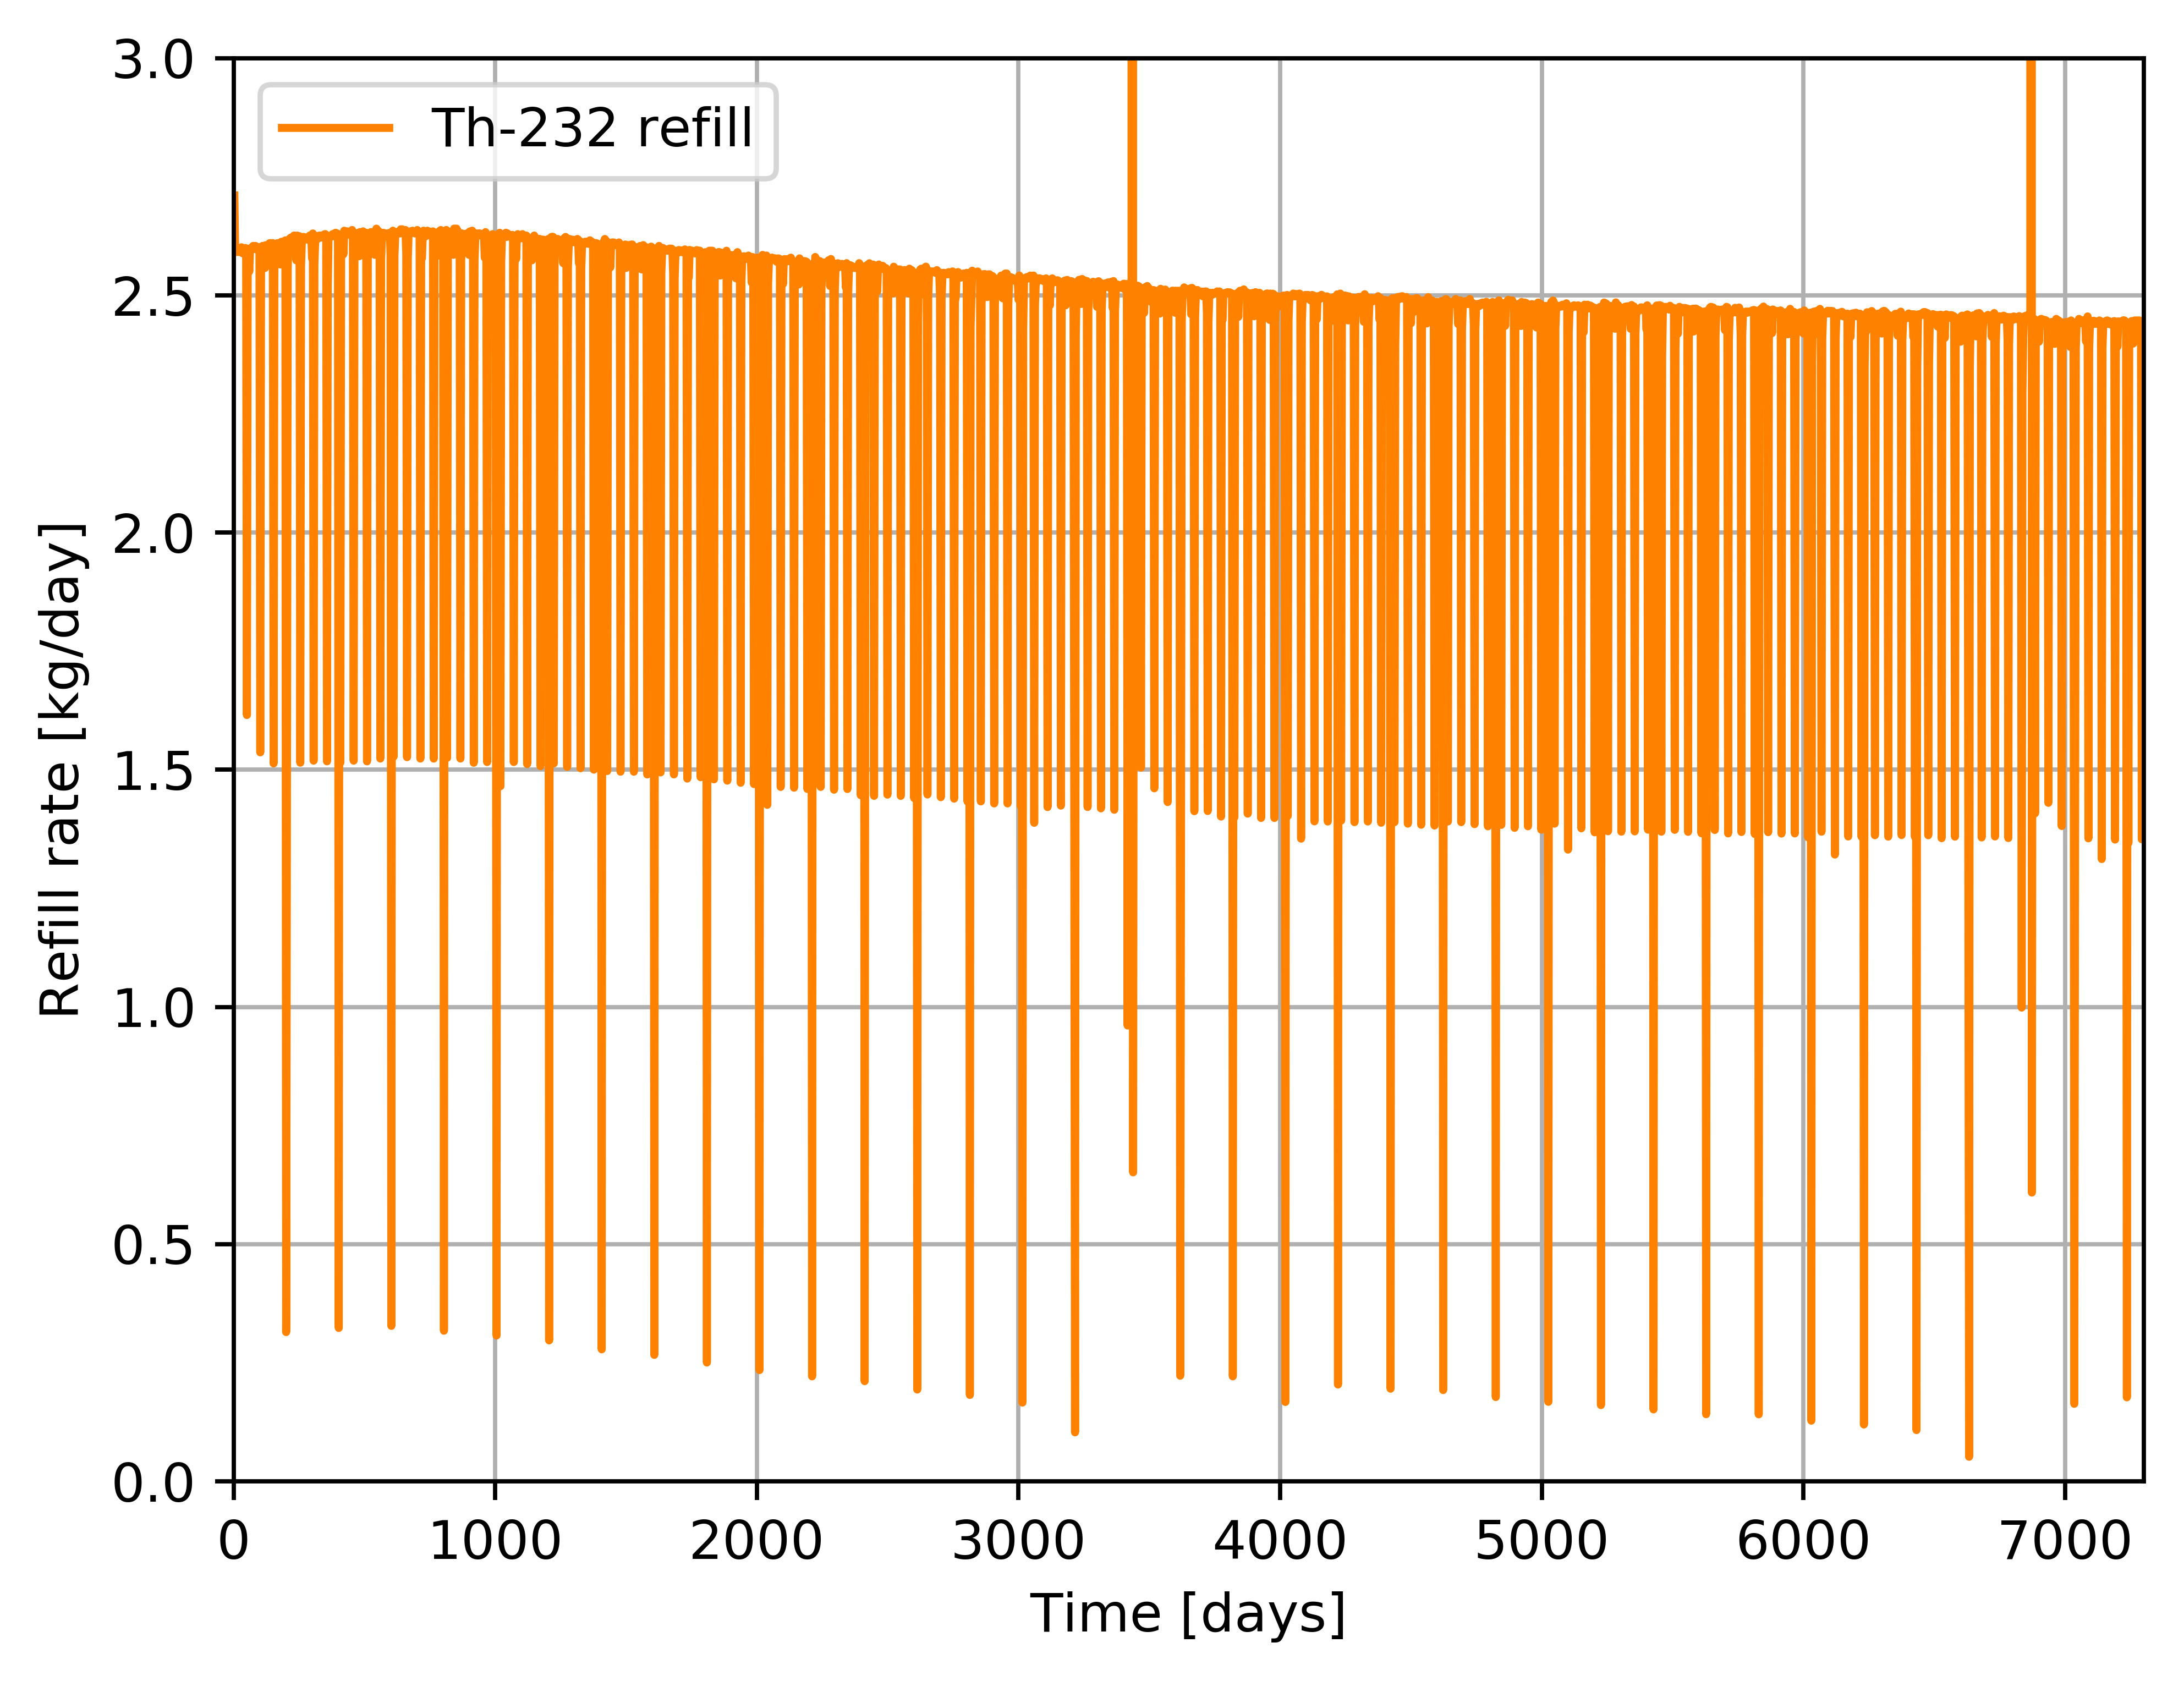
\includegraphics[width=\textwidth]{Th_refill_rate.png} 
      \vspace{-1.5em}
  \caption{$^{232}$Th feed rate over 20 years of \gls{MSBR} operation.}
    \vspace{-0.6em}
  \label{fig:th_refill}
\end{figure}
\begin{figure}[htp!] % replace 't' with 'b' to force it to 
  \centering
    \vspace{-0.3em}
  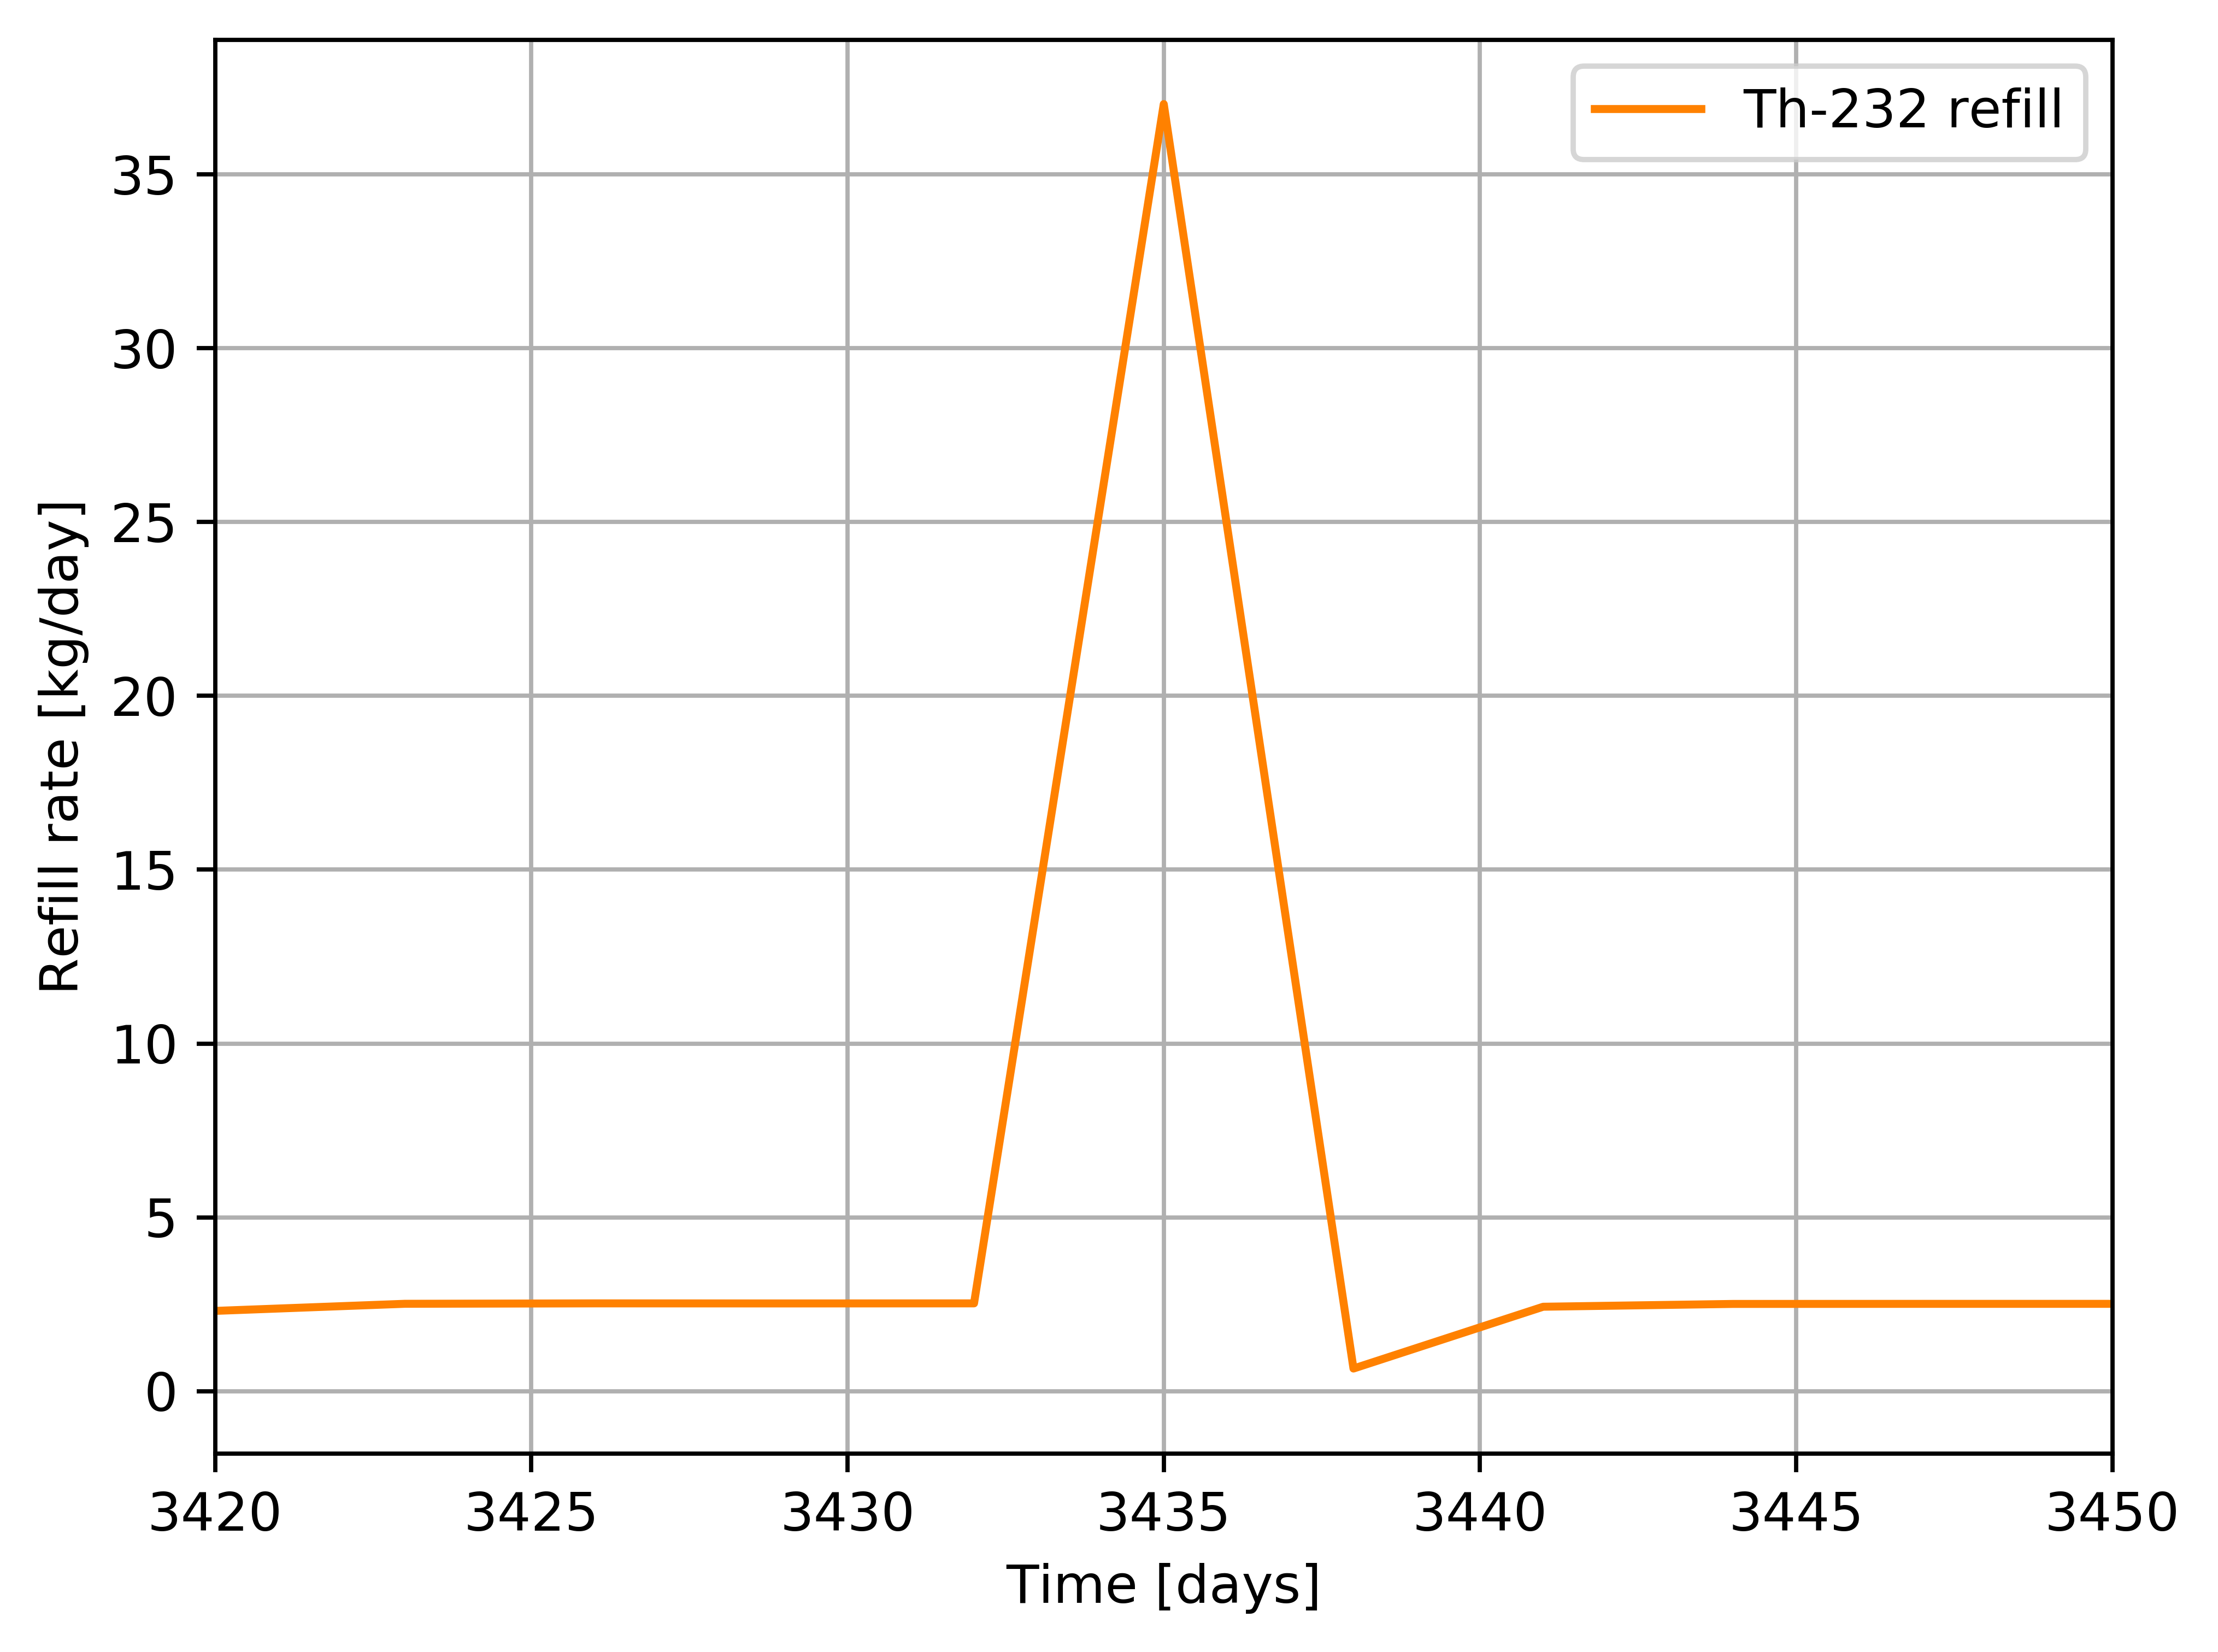
\includegraphics[width=\textwidth]{Th_refill_rate_spike.png} 
      \vspace{-1.5em}
  \caption{Typical $^{232}$Th feed rate spike caused by strong absorbers (Rb, Sr, Cs, Ba) removal.}
    \vspace{-0.6em}
  \label{fig:th_refill_spike}
\end{figure}
\FloatBarrier

\chapter[Conclusions and furture work]{Conclusions and future work}
This thesis introduces the open source \gls{MSR} simulation code SaltProc. The SaltProc modeling and simulation tool expands the capability of a continuous-energy Monte Carlo Burnup calculation code SERPENT 2 for simulating liquid-fueled \gls{MSR} operation \cite{andrei_rykhlevskii_arfc/saltproc:_2018}. Benefits of SaltProc include generic geometry modeling, multi-flow capabilities, time-dependent feed and removal rates, and ability to specify removal efficiency. The main goal has been to assess the ability of this tool to find equilibrium fuel salt composition (e.g., number density of major isotopes vary less than 1\% over several years). A secondary goal has been to compare predicted operational and safety parameters (e.g., neutron energy spectrum, power and breeding distribution, temperature coefficients of reactivity) of the \gls{MSBR} at initial and found equilibrium state. A tertiary study goal has been to demonstrate and prove that in one-fluid two-region \gls{MSBR} conceptual design the outer core zone II serves as breeding ``blanket" to catch leaked from the central core zone I neutrons and improve breeding ratio.

In order to assemble the SaltProc tool, a full-core high-fidelity benchmark model of the \gls{MSBR} was implemented in the SERPENT 2. The purpose of the full-core fidelity model instead of simplified single-cell model \cite{rykhlevskii_online_2017}, \cite{betzler_molten_2017} was to precisely describe two-region \gls{MSBR} concept design that allowed accurately represent breeding in a ``blanket" (outer core zone). When running depletion calculation, the most important fission products and $^{233}$Pa are removed and fertile/fissile materials are added to fuel salt every 3 days while rare earths, volatile flourides and seminoble metals removal interval was more than month. 

The results of this study indicate that from the depletion calculation the effective multiplication factor slowly decreases from 1.075 and reaches to the equilibrium state with the factor about 1.02 after approximately 6 years of operation. At the same time, concentration of $^{233}$U, $^{232}$Th, $^{233}$Pa, $^{232}$Pa composition changes insignificantly after approximately 2500 days of operation. Particullarly, $^{233}$U number density fluctuates less than 0.8\% from 16 to 20 years of operation, consequently, it might be assumed that the core reaches to the quasi-equlibrium state after 16 years of the fuel irradiation. On the other hand, wide diversity of nuclides, including fissile isotopes (e.g. $^{233}$U, $^{239}$Pu) and non-fissile strong absorbers (e.g. $^{234}$U), keep accumulating in the core. The results in this thesis shows that trully equilibrium materials composition cannot exist but the balance between negative effects of strong absorbers accumulation and new fissile materials production might be achieved to keep the reactor critical.

The next most obvious finding to emerge from the analysis of initial and equilibrium materials composition is that neutron energy spectrum is harder for equilibrium state because significant amount of heavy fission products were accumulated in the \gls{MSBR} core. Moreover, neutron energy spectrum in the central core region is much softer than in outer core region due to lower moderator-to-fuel ratio in outer zone, and this distribution not changes during reactor operation. Finally, the epithermal and thermal spectrum needed to effectively breed $^{233}$U from $^{232}$Th because radiative capture cross section of thorium-232 monotonically decreases from $10^{-10}$ MeV to $10^{-5}$ MeV. Harder spectrum in the outer core region tends to significantly increase resonance absorption in thorium and decrease the absorptions in fissile and construction materials. 

The calculated heat power spatial distribution of the \gls{MSBR} shows that 98\% of the fission power is generated in central zone I, and neutron energy spectral shift did not cause any notable changes in power distribution. The neutron capture reacton rate spatial distribution for fertile $^{232}$Th, which quantified breeding in the core, confirms that the most of breeding occurs in an outer, undermoderated, region of the \gls{MSBR} core. Moreover, calculated thorium-232 feed rate gradually decreases from about 2.7 kg/day at the beginning of operation to 2.4 kg/day at the end of 20-years timeframe. Finally, the average $^{232}$Th refill rate throughout 20 years of operation is approximately 2.39 kg/day or 100 g/GWh$_e$ in this study which is a good agreement with most recent online reprocessing analysis by \gls{ORNL} \cite{betzler_molten_2017}.

Comparisons of the safety parameters were made for initial fuel loading and equilibrium materials composition with SERPENT 2 code. It is noted that neutron energy spectrum hardening over the fuel depletion and this spectral shift couses changes in the reactor behaviour. The total temperature coefficient is relatively large and negative at the initial and equilibrium state but the magnitude decreases throughout reactor operation from $-3.10$ to $-0.94$ pcm/K, and moderator temperature coefficient is positive and also decreases during fuel depletion. From reactivity control system efficiency results, the safety rod integral worth decreases by approximately 16.2\% over 20 years of operation, while graphite rod integral worth staying the same. Summing up, neutron energy spectrum hardening during fuel salt depletion has considerable negative impact on \gls{MSBR} stability and controllability, and should be taken into consideration in further analysis of accident transient scenarios.

Continued research into SaltProc-SERPENT 2 and related topics could progress in a number of different directions. First and foremost efforts should be made at reprocessing parameters (e.g. time step, feeding rate, protactinium removal
rate) optimization to achieve the best fuel utilization, breeding ratio or safety characteristics. This might be performed using additional script which would change input parameter by small increment, run workbench and analyse output to determine optimal configuration. Furthermore, existing optimisation framework RAVEN might be employed for this optimisation study \cite{alfonsi_raven_2013}.

Only the semi-batch online reprocessing approach has been treated in this thesis. However, SERPENT 2 Monte Carlo code recently was extended for trully continuous online fuel reprocessing simulation \cite{aufiero_extended_2013}. This extension must be verified against existing SaltProc/SERPENT or ChemTriton/SCALE workbench, and could be employed to immediate removal of fission product gases (e.g., Xe, Kr) which has strong negative impact on core lifetime and breeding efficiency. Finally, using build-in SERPENT 2 Monte Carlo code online reprocessing \& refueling material burnup routine would significantly speedup computer-intensive full-core depletion simulations.

Lastly, an additional area to explore is the accident safety analysis which requires to develop multi-physics model of \gls{MSBR} in the coupled neutronics/ thermal-hydraulics code Moltres \cite{lindsay_introduction_2018}. Existing full-core SERPENT 2 model and equilibrium fuel material composition would be employed to problem-oriented nuclear data libraries generation for further usage in accident transient analysis. The final goal of this effort is develop fast-running computational model which would aim at studying the dynamic behavior of generic \gls{MSR}, performing detailed safety analysis and design optimization.



%%%%%%%%%%%%%%%%%%%%%%%%%%%%%%%%%%%%%%%%%%%%%%%%%%%%%%%%%%%%%%%%%%%%%%%%%%%%%%%
% APPENDIX
%
%\appendix
%\include{apx}

\backmatter

%%%%%%%%%%%%%%%%%%%%%%%%%%%%%%%%%%%%%%%%%%%%%%%%%%%%%%%%%%%%%%%%%%%%%%%%%%%%%%%
% BIBLIOGRAPHY
%
%\bibliographystyle{IEEE_ECE}
\bibliographystyle{unsrt}
% Put references in BibTeX format in thesisrefs.bib.
\bibliography{thesisrefs}

\end{document}
\endinput
